\documentclass[letterpaper,12pt]{report}
\usepackage{palatino,url,graphicx}
\usepackage[utf8]{inputenc}
\usepackage{amsmath}
% \usepackage[ruled,vlined]{algorithm2e}
\usepackage{setspace}
\usepackage{appendix}
\usepackage[graph, frame]{xy} % For X-MIMI prbac Chapter
\usepackage[final]{pdfpages}
\usepackage{listings}
\usepackage{pgf,tikz}
\usetikzlibrary{shapes,arrows,snakes,automata,backgrounds,trees,calc,matrix,positioning,fit}
\usepackage{colortbl}
\usepackage{enumerate}
%\usepackage[lined,boxed,linesnumbered]%{algorithm2e}
%\usepackage{algorithmic}
\usepackage{boxedminipage}
\usepackage{multirow}
\usepackage{url}
\usepackage[font={small,it}]{caption}
\usepackage{rotating}
\usepackage{array}
\usepackage{pdflscape}

\usepackage{moreverb}
\usepackage{bm}

\usepackage{algpseudocode}
\usepackage{algorithm}
\lstset{
	%language=ruby,
	keywordstyle=\bfseries\ttfamily\color[rgb]{0,0,1},
	identifierstyle=\ttfamily,
	commentstyle=\color[rgb]{0.133,0.545,0.133},
	stringstyle=\ttfamily\color[rgb]{0.627,0.126,0.941},
	showstringspaces=false,
	basicstyle=\small,
	numberstyle=\footnotesize,
	numbers=none,
	stepnumber=1,
	numbersep=10pt,
	tabsize=2,
	breaklines=true,
	prebreak = \raisebox{0ex}[0ex][0ex]{\ensuremath{\hookleftarrow}},
	breakatwhitespace=false,
	aboveskip={1.5\baselineskip},
  columns=fixed,
  extendedchars=true,
% frame=single,
% backgroundcolor=\color{lbcolor},
}

% http://www.tug.org/applications/hyperref/manual.html
\usepackage[breaklinks=true]{hyperref}
\hypersetup{
   bookmarks=false,         % show bookmarks bar?
%    unicode=false,          % non-Latin characters in Acrobat‚ bookmarks
%    pdftoolbar=true,        % show Acrobat‚ toolbar?
%    pdfmenubar=true,        % show Acrobat‚ menu?
%    pdffitwindow=false,     % window fit to page when opened
%    pdfstartview={FitH},    % fits the width of the page to the window
   pdftitle={LOCALIZING FAULTS IN NUMERICAL SOFTWARE USING A VALUE-BASED CAUSAL MODEL},    % title
   pdfauthor={Zhuofu Bai},     % author
   pdfsubject={Ph.D. Dissertation},   % subject of the document
   % pdfcreator={TextMate},   % creator of the documentt
%    pdfproducer={Producer}, % producer of the document
%    pdfkeywords={keywords}, % list of keywords
%    pdfnewwindow=true,      % links in new window
   colorlinks=true,       % false: boxed links; true: colored links
   linkcolor=black,          % color of internal links
   citecolor=black,        % color of links to bibliography
   filecolor=black,      % color of file links
   urlcolor=black           % color of external links
}


\input xy
\xyoption{all}

\doublespacing

\setlength\oddsidemargin{0.5in}
\setlength\textwidth{6.0in}
\setlength\topmargin{0in}
\setlength\headheight{0in}
\setlength\headsep{0in}
\setlength\textheight{9in}
%%sets the textwidth to 6.5, which leaves 1 for the remaining right margin with 8 1/2X11inch paper
\DeclareUnicodeCharacter{00A0}{ }

\begin{document}
  \pagenumbering{roman}

% UNCOMMENT BELOW
\title{LOCALIZING FAULTS IN NUMERICAL SOFTWARE USING A VALUE-BASED CAUSAL MODEL}
\author {by\\ZHUOFU BAI}
\date{\vspace{0.8cm}Submitted in partial fulfillment of the requirements\\
For the degree of Doctor of Philosophy\\
\vspace{0.45in}
Dissertation Advisor: Andy Podgurski\\
\vspace{0.45in}
Department of Electrical Engineering and Computer Science\\
CASE WESTERN RESERVE UNIVERSITY\\
\vspace{0.45in}
TBD}

\maketitle

% Committee Signature sheet (typed version)-originals turned in with Final Materials
% \includepdf{signature_sheet_filled_in.pdf}

% % Copyright page (only if copyrighting)
% \newpage
% Copyright page (only if copyrighting)

% % Dedication page (optional)
% \newpage
% Dedication page (optional)

% \singlespacing
%% UNCOMMENT BELOW
\setcounter{page}{3}
\tableofcontents
\listoftables
\listoffigures

% \doublespacing
%% UNCOMMENT BELOW
% % Preface (optional)
% \newpage
% Preface (optional)
% Acknowledgements (optional)

\newpage
\section*{Acknowledgements}
First and foremost, I would like to thank my advisor, Dr. Andy Podgurski for his constant support and guidance.  Dr. Podgurski led me into the field of software testing and reliability and guided me in every project. He is  knowledgable, responsible and patient.  Especially in the first few years of my PhD, I was stuck on my research and almost give up. Dr Podgurski shared his innovative ideas with me, and contributed a lot of time to help overcome the difficulties in my research. Everything would be different without him. 

My sincere thanks also go the members of my committee, Dr. Soumya Ray,  Dr. M. Cenk Cavusoglu and Dr. Xiang Zhang for their invaluable feedback, scientific suggestions and insightful discussions, which helped me improve this dissertation. I would like to give special thanks to Dr. Soumya Ray, who generously offered advices and shared research experiences with me during my Ph.D. study.

I would like to thank all my co-workers at Case Western Reserve University: Dr. Boya Sun, Dr. Gang Shu, Shih-feng Sun, Dr. Mark Renfrew, Feng Cao, Kai Liang,  Erdem Tuna. This work will be impossible without their support and cooperation. I am thankful to my close friends, Jiangli Zhu, Yang Zhang, Jiale Li, Xuefei Wang. 

I deeply appreciate my parents, Xiaomin Wang and Baodong Bai, for their unconditional love and support. My wife, Yang Chen, always encourage me and gives me her best possible support. Thank you, Yang. I couldn’t have done it without you. 



% List of Abbreviations (optional)
\newpage
\section*{List of Abbreviations}
\begin{itemize}
  \item OMIM: Online \lowercase{Mendelian Inheritance in Man}
  \item GWAS: Genome-wide association study
  \item UMLS: Unified \lowercase{Medical Language System}
  \item CBIR: Content-based image retrieval
  \item SIFT: Scale invariant feature transformation
  \item HOG: Histograms of oriented gradients
  \item SVM: support vector machine
  \item HPRD: Human \lowercase{Protein Reference Database}
  \item PPI: Protein-protein interaction
  \item HDN: Human disease network
  \item CRC: Colorectal cancer
  \item PD: Parkinson's disease
  \item DMN: Disease manifestation network
  \item IMPC: International \lowercase{Mouse Phenotyping Consortium}
  \item FDA: Food and drug administration

\end{itemize}

% % Glossary (optional)
% \newpage
% Glossary (optional)

\newpage
\begin{centering}
  Localizing Faults in Numerical Software Using a Value-Based Causal Model
  LOCALIZING FAULTS IN NUMERICAL SOFTWARE USING A VALUE-BASED CAUSAL MODEL\\
  \vspace{1cm}
  Abstract\\
  by\\
  \vspace{1cm}
  Zhuofu Bai\\
  \vspace{1cm}
\end{centering}



Causal statistical fault localization (CSFL) technique, for example, Baah et al’s causal regression model, has been approved to be effective in localizing software faults with test profiles and outcome. In most research on CSFL, execution dynamics have been characterized by code-coverage profiles, indicating which statements, branches, or paths were covered by each execution. This coverage based CSFL has two potential problems: (1) The cause effect estimation can be biased when the positivity condition is violated  (2) It poorly suited for localizing faults in numerical programs and subprograms having relatively few conditional branches. 

To solve the above problems, we first investigates the performance of Baah et al’s causal regression model for fault localization when an important precondition for causal inference, called positivity, is violated.  Two kinds of positivity violations are considered: structural and random ones.  We prove that random, but not structural nonpositivity may harm the performance of Baah et al’s causal estimator.  To address the problem of random nonpositivity, we propose a modification to the way suspiciousness scores are assigned.  Empirical results are presented that indicate it improves the performance of Baah et al’s technique. We also present a probabilistic characterization of Baah et al’s estimator, which provides a more efficient way to compute it.

Then we proposed two value-cased causal inference models for localizing faults in numerical software. The first model is NUMFL. NUMFL combines causal and statistical analyses to characterize the causal effects of individual numerical expressions on output errors.  Given value-profiles for an expression's variables, NUMFL uses generalized propensity scores (GPSs) or covariate balancing propensity scores (CBPSs) to reduce confounding bias caused by evaluation of other, faulty expressions.  It estimates the average failure-causing effect (AFCE) of an expression using quadratic regression models fit within GPS or CBPS subclasses.  We report on an empirical evaluation of NUMFL involving components from four Java numerical libraries, in which it was compared to five alternative statistical fault localization metrics.  The results indicate that NUMFL is more effective than baseline techniques. We also found that NUMFL works fairly well with data from failing runs alone. 

The second model is Bayesian Additive Regression Trees (BART) model. Instead of controlling confounding bias with propensity scores, BART model fits a sum of trees structure to approximate the dose response function (DRF) of both treatment variable and the confounding variables. For every unit in the observational data set of an expression, BART model estimate the causal effect of treatment variable on outcome with the fitted sum of trees structure. The average value of the estimated causal effect of each unit in data set is the estimated AFCE of the expression. We compare the performance of BART model with that of NUMFL and five baseline techniques in empirical evaluation. The result shows BART model is the most effect techniques overall.  But the computation cost of BART model is more expensive than NUMFL and other baseline techniques.











% Remember: Motivation, Pros and Cons, Lessons Learned

% TODO: Search for they're their there, where were
% Already checked: it's and its, don't => do not, your, you're


%---------------------------Chapters---------------------------------%
\newpage
\pagenumbering{arabic}
\chapter{Introduction}\label{chap:introduction}
\section{Statistical Fault Localization}
Typical SFL techniques take data characterizing a set of both passing and failing program executions, including PASS/FAIL labels (provided by testers or end users) and recorded profiles of internal program dynamics, and they compute statistical measures of the strength of the association, if any, between the occurrence of software failures and the occurrence of certain runtime events at particular program locations.  These measures are then used to help guide the search for the causes of observed failures, typically by ranking program statements by the strengths of their associations with failures.  When SFL techniques are evaluated they are generally used as the sole source of information about possible fault locations.  However, it seems more realistic to envision them ultimately being used in combination with other sources of information, such as programmer hunches and {\it fault prediction models} \cite{Fenton1999} based on static code properties and project history.  Potentially, SFL techniques provide a relatively inexpensive way to maximize the information obtained by testing.


\section{Bugs in Numerical Software}
Numerical software plays a very important role in science, industry, and defense, and failures of numerical software have been reported as the cause of several well-publicized ``disasters" \cite{VuikWeb,Kanewala2014}.  However, automated techniques intended specifically for localizing numerical faults based on execution data have received relatively little attention from researchers, although there has been substantial research on general {\it statistical fault localization} (SFL) techniques (e.g. \cite{Jones2002,Liblit2004,Liu2005}) and on other general automated debugging techniques (see Section 3.6).

The numerical bugs in the software are often hard to detect because they may not necessarily result in software crashes. It is very difficult to localize the fault by tracing back the execution, because we lack the oracle of intermediate variable values. Testers usually detect failures in numerical program by checking whether the difference between the program output and expected output exceeds a pre-defined tolerance.

\section{Causal Inference with Statistical Fault Localization}
Coverage-based statistical fault localization (SFL) techniques apply statistical or machine learning techniques to code-coverage profiles (or ``spectra") and PASS/FAIL labels for a set of observed program executions, in order to identify possible locations of the fault(s) that caused some of the executions to fail.  These techniques equate the ``suspiciousness" of a program element with a statistical measure of the association between coverage of that element and the occurrence of program failures.  For example Baah et al showed \cite{baah2010causal} that the Tarantula metric \cite{jones2002visualization}, the Ochiai metric \cite{abreu2007accuracy}, and the F1-measure \cite{baah2010causal} each embed an estimator of the conditional probability of program failure given that a statement  is covered, which we denote by $P(F|s)$.  

It should be noted, first of all, that these and other suspiciousness metrics do {\it not} directly estimate the probability that is {\it faulty}, because doing so would require data about observed faults, not just data about {\it failures}.  One might hope instead that such suspiciousness metrics yield good estimates of the {\it average causal effect} \cite{pearl2000models} of executing a given program element on the occurrence of failures, which we shall call the {\it average failure-causing effect} (AFCE).  Average causal effect estimates are used to study causality in a variety of fields, such as epidemiology, econometrics, and social science.  However, as Baah et al pointed out \cite{baah2010causal}, SFL suspiciousness metrics often produce biased estimates of a program element’s AFCE, due to the effects of other program elements.  For example, Figure \ref{fig2.1} shows a small function that contains a bug in statement $s_3$, which should be $y=x+2$.  Appropriately, $P(F|s_3)=1$.  However, because the faulty statement $s_3$ is always executed before either of the correct statements $s_5$ or $s_8$ is executed, $P(F|s_5)=P(F|s_8)=1$, which suggests misleadingly that $s_5$ and $s_8$ are faulty.

\begin{figure}[htb!]
\vspace{0em}
\begin{center}
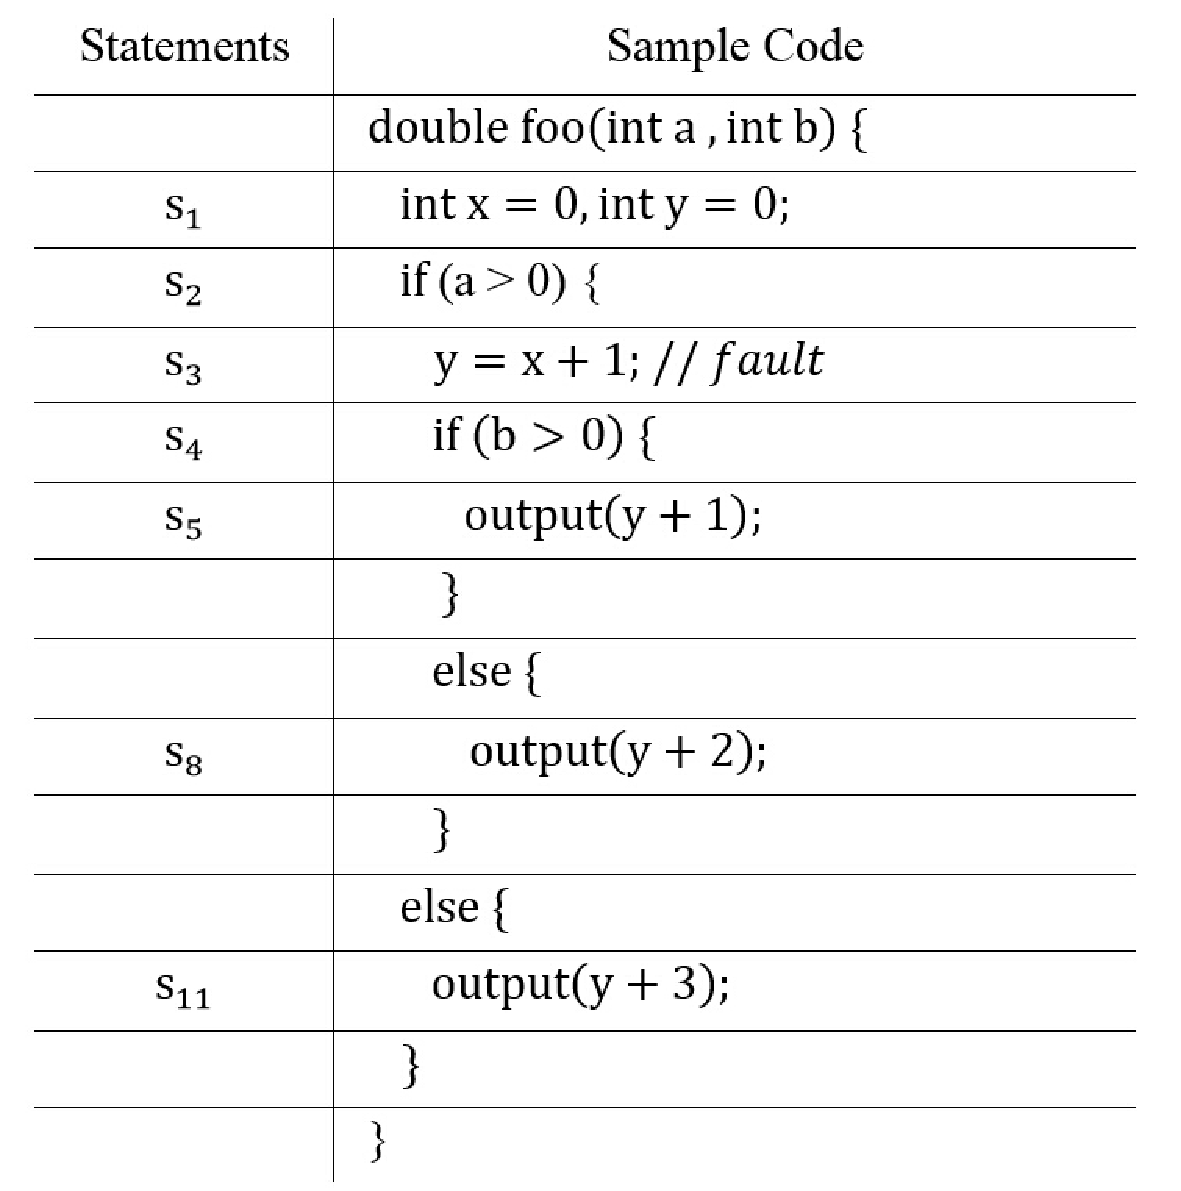
\includegraphics[width=0.6\textwidth]{chapter2_fig1.pdf}
\vspace {0em}\caption{Motivating Example} \label{fig2.1}
\end{center}
\vspace {0em}
\end{figure}

This problem, which is an instance of {\it confounding bias} (or just {\it confounding}) \cite{pearl2000models}, is due to the fact that execution of the control dependence region \cite{ball1993s} containing statements $s_3$ and $s_4$ is a {\it common cause} of program failure and of execution of statement $s_5$ or $s_8$.  More generally, confounding of the effect of a ``treatment" variable $T$ on an outcome variable $Y$ is bias due to the presence of a common cause $C$ of $T$ and $Y$.  Confounding bias cannot be eliminated, in general, without considering the causal relationships between the variables under study.  These relationships are typically represented in a {\it causal} DAG \cite{pearl2000models}, which is a directed acyclic graph in which there is an edge $A \rightarrow B$ just in case variable $A$ is a direct cause of variable $B$.  For example, Figure \ref{fig2.2} is a very simple causal graph showing the causal relationships between a treatment $T$, an outcome $Y$, and a confounder $C$.  For SFL, Baah et al \cite{baah2010causal,baah2011mitigating} proposed using a causal DAG derived from the {\it program dependence graph} (PDG) \cite{ferrante1987program}, in which the nodes represent binary coverage indicator variables.

Confounding can be reduced or eliminated by adjusting or controlling for a suitable set of variables during statistical analysis.  A well-known result of Pearl, the {\it Back-Door Adjustment Theorem} \cite{pearl2000models}, states that a set of covariates $\mathbf{X}$ in a causal DAG $G$ is sufficient for confounding adjustment if it ``blocks" all ``backdoor paths" between the treatment $T$ and the outcome $Y$.  A {\it backdoor path} between $T$ and $Y$ is a path with an arrow $T \leftarrow$ entering $T$.  A path is {\it blocked} by $mathbf{X}$ if the path (1) contains a configuration of the form $\rightarrow Z \rightarrow$ or $\leftarrow Z \rightarrow$ such that  $Z \in \mathbf{X}$or (2) contains a ``collider" $\rightarrow Z \leftarrow$  such that neither $Z$ nor any of its descendants is in $\mathbf{X}$.  For example, in Figure \ref{fig2.2} the path $T \leftarrow C \rightarrow Y$ is a backdoor path, which is blocked by $C$.

\begin{figure}[htb!]
\vspace{0em}
\begin{center}
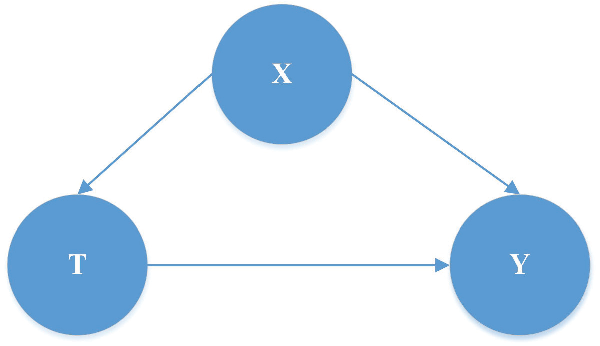
\includegraphics[width=0.6\textwidth]{chapter2_CausalDAG1.pdf}
\vspace {0em}\caption{Causal Diagram of treatment, outcome and confounder} \label{fig2.2}
\end{center}
\vspace {0em}
\end{figure}

\section{Contribution and organization of the dissertation}

This dissertation makes the following contributions: developed a novel value based approach to to SFL for numerical programs; analyzed two types of violations of positivity: structural violations and random violations in casual fault localization; the first use of BART model to estimate failure-causing effect for numerical expressions.

The remainder of the dissertation is organized as follows:

Chapter 2 investigates the performance of Baah et al’s causal regression model for fault localization when positivity condition is violated

Chapter 3 presents a value based causal inference model for localizing faults in numerical software called NUMFL, which use propensity score technique to control the confounding bias in fault localization.

Chapter 4 presents a new fault localization method based on Bayesian additive regression trees model.

Chapter 5 presents an approach to automatically localize faulty statements in the embedded control software.

Chapter 6 concludes this dissertation and discusses the possible improvements for future work.





%\chapter{Ontology guided approach to retrieving medically-relevant web images: application on retrieving disease manifestation images}\label{image2}

\section{Motivation}
Towards the goal of constructing a patient-oriented health image base,
we propose a content-based image retrieval (CBIR) method
to retrieving disease manifestation images from the web.
The image retrieval task is highly challenging, since disease manifestation
images contain diverse objects and complex backgrounds.
For example, the positive examples of ``hand,
foot, and mouth disease" may contain infected feet,
hands, mouths, or tongues. The body parts are in
different positions and sizes, and more
than one infected body part may appear in one
single image. To collect disease images from the
web, we need to analyze the image at the object
level at the minimal cost of manual effort.
%\begin{figure}[htb!]
%\vspace{0em}
%\begin{center}
%\includegraphics[width=0.8\textwidth]{Chap2_handfootmouth.eps}
%\vspace {0em}\caption{Positive examples of images on hand, foot, and mouse disease.} \label{handfootmouth}
%\end{center}
%\vspace {0em}
%\end{figure}

Most CBIR systems apply machine learning approaches to
bridge the semantic gap between image content and users' interpretations \cite{datta2008image}.
These approaches include supervised classification \cite{chapelle1999support},
similarity-based clustering \cite{li2008real}, semi-supervised
co-training \cite{feng2004bootstrapping}, and active learning based on relevant feedback \cite{tong2001support}.
A few methods incorporated additional information to improve
retrieval precision. For example, Deserno {\it et al} exploited
figure types and panel numbers to retrieve literature figures \cite{deserno2009content}.
Muller {\it et al} summarized the retrieval methods for integrating
texts with image content \cite{muller2012overview}.
Simpson {\it et al} combined natural language
and image processing to map regions in CT scans to concepts
in RadLex ontology, which was automatically extracted
from image captions \cite{simpson2012towards}.
Deng {\it et al} used semantic prior knowledge
to retrieve similar images \cite{deng2011hierarchical}. One particularly relevant
method of reducing human effort in health image collection is
the bootstrap image classification method \cite{chen2012semi}. This approach uses
one positive sample as the ``seed" to iteratively retrieve more
positive images, and thus is appropriate for large-scale image
collection. Although this approach effectively collects human
organ and drug images, it has limited precision for disease
images \cite{chen2012semi}. Because web images are highly heterogeneous, our
task requires supervision of the training data to ensure good
precision. However, traditional supervised methods need a training
image set for each disease, thus will not scale up
when the number of disease terms is large.

To solve the scalability problem, we propose an ontology-guided
organ detection method to collect disease manifestation
images from the web. Based on observation, we assume that
most disease manifestation images contain abnormal human
body parts, such as eyes, ears, and hands, which show visible
disease symptoms. Therefore, our approach uses the existence
of these body parts to discriminate between images of disease
and non-disease images. Instead of training a classifier for each
disease, we pretrain a set of organ detectors, each of which
detects one target organ. When retrieving images for a given
disease, we extract the disease-organ semantic relationships
from ontologies, and use the corresponding detectors to detect
associated organs from web images.

Our method has two major advantages. First, we require much
fewer training data than the standard supervised method, which
trains a classifier for each disease, because we reuse organ detectors
across diseases. For example, 428 diseases in the UMLS
record eyes. Instead of training 428 classifiers, one for each
disease, we train one detector for ``eye" and reuse it to classify
428 types of eye disease images. Second, our approach achieves
high accuracy when disease images contain diverse manifestations
of different organs, such as images of ``hand, foot, and mouth
disease." For each disease, we use prior knowledge of disease-
organ associations as guidance to scan images at the object level.


\section{Data and methods}

Fig. {\ref{Chap2_system}}A shows the steps of the method. For a given disease, we first use the UMLS to determine what body parts the disease is manifested on. Then we use a set of pre-trained body part detectors, using state-of-the-art image features, to find the targets at multiple scales. Finally we combine the scanning results of each detector at all scales into high level features to classify the input images as relevant or irrelevant.
\begin{figure}[t]
\vspace{0em}
\centering
\includegraphics[width=\textwidth]{Chap2_system.eps}
\vspace {0em}\caption{(A) The Overview of disease image retrieval approach. We use the UMLS to determine the body part locations of disease manifestations and to select from a set of pre-trained body part detectors to filter Google search results into relevant and irrelevant images. Comparing to a supervised method that would require labeled training examples for each disease, we achieve high precision in image retrieval while reducing human effort to a minimum. (B) The structure of organ detectors. Our decision rule is based on multiple objects detectors at multiple scales. It is crucial to have multiple scales because some disease images have body parts occupying the entire frame, while others include a large portion of the background.}
\label{Chap2_system}
\vspace {0em}
\end{figure}


\subsection{Discovering target body parts}
For each target disease, we find its corresponding body parts through the UMLS semantic network relationship of ``has\_finding\_site". One body part is typically associated with at least hundreds of diseases; this fact shows that reusing common body part detectors across diseases can save a huge amount of human labeling effort. Each disease can have manifestations on multiple body parts:  among the diseases that involve the ``has\_finding\_site" relation in UMLS, around 15\% of them are located on more than one body parts. For such complex diseases, we will combine the detection results of multiple body parts into high level features to boost the retrieval precision.

Some diseases affect internal organs that are not directly visible in images. Nonetheless, symptoms on these organs can have direct manifestation on external body parts. We manually map part internal organs to their associated external body parts by using the ``isa" and ``part\_of" relationships in the UMLS. For example, the ``oral mucous membrane structure" is a part of the ``entire mouth region", which is a synonym of ``mouth" in the UMLS. Thus diseases having the symptoms in ``oral mucous membrane structure" are considered to be associated with ``mouth". In addition, some diseases are located on body parts that are too detailed according to the UMLS. We also manually map such body parts to the larger organs that contain them based on the ``part\_of" relationship. For example, ``upper eye lid" and ``lower eye lid" are parts of ``eye", therefore are mapped to ``eye". Diseases manifested on upper and lower eyelids then have ``eye" as the target body part.

\subsection{Detecting target body parts}
We develop a general human organ detection method, and adapt it to specific targets by tuning training data as well as parameters. Currently, we have trained detectors for eye, ear, lip/mouth, hand and foot, and reused them in retrieving images of a variety of diseases. The detectors are learned in a generic way and can be easily extended to other body parts.

Object detection is a fundamental problem in computer
vision. Approaches to object detection typically consist of two
major components: feature extraction and model construction.
Lowe developed the scale invariant feature transformation
(SIFT) as the image patch descriptor \cite{lowe1999object}.
Dalal and Triggs \cite{dalal2005histograms} proposed
the histograms of oriented gradients (HOG) for human
detection. These features have proved effective in object detection
applications. In addition, Zhang {\it et al} constructed a
bag-of-feature model to classify texture and object categories \cite{zhang2007local}.
Felzenszwalb {\it et al} developed a generic object detector with
deformable part models to handle significant variations in object
appearances \cite{felzenszwalb2010object}.


Fig. {\ref{Chap2_system}}B shows the structure of our organ detector. Each
detector $i (i=A, B…)$ detects one target organ using multiple
classifiers. Each classifier $C_{ij}$ scans the input image and searches
for the target at detection scale $j ( j=1, 2…)$. For example, if
detector $A$ is an eye detector and contains three classifiers, then
$C_{A1}$ decides if the full image is an eye, $C_{A2}$ scans the image with
a detection window to search for small eyes, and $C_{A3}$ searches
for eyes of an even smaller size. The organ detection results
${S_{A1}, S_{A2}, ..., S_{B1}, S_{B2}}$ are binary values and represent the
existence of each organ $\{A,B,\cdots\}$ at each detection scale $\{1,2,\cdots\}$.
We then combined these results into high-level features,
based on logic, to make final decisions about the input images.
We found that the accuracies of our simpler detection system
were comparable to that of Felzenszwalb et al \cite{felzenszwalb2010object}.



\subsubsection{Training organ detectors}
For all classifiers in each organ detector, the training samples
consisted of web images collected by Google. To collect positive
examples, we searched the six body part names as the keywords
and manually picked 200--300 images of the body part itself
with little background. Most positive examples are not medically
relevant, but contain different views of the body parts. To
collect negative images, we summarized the categories of objects
and backgrounds that often appear in the Google query results,
such as paper snapshots, animals, and buildings. Negative examples
were then collected by searching keywords such as ``research
paper," ``dog," and ``building." Five thousand images comprised
the negative training set. We used the same negative examples
for all the organ detectors.

We trained three standard soft margin support vector
machine (SVM) classifiers for each organ detector to detect
targets on three scales. In detector i, $C_{i1}$ was trained by full
training images. Since $C_{i2}$ and $C_{i3}$ search for targets with detection
windows, they used positive samples that were resized to
the window sizes, and randomly selected image patches of the
window sizes from negative samples. We extracted the HOG
features \cite{dalal2005histograms} from training images. The HOG is reminiscent of the
SIFT descriptor, but uses overlapping local contrast normalizations
for improved performance \cite{dalal2005histograms}. The window sizes of $C_{i2}$ and
Ci3 were empirically chosen as $64 \times 96$ pixels and $32 \times 48$ for
eye, lip/mouth, and hand detectors; and $96 \times 64$ and $48 \times 32$ for
foot and ear detectors. By browsing 100 eye disease images, we
found that images containing only very small target organs were
usually false positives, therefore did not train classifiers at any
smaller scale in order to maintain high retrieval precision.



\subsection{Combining detections for disease image classification}
We finally used the organ detection results that represent the
existence of affected organs as high-level features to classify the
input images into disease or non-disease categories. Ideally, if all
the classifiers behave in the same way and are independent, the
high-level combined feature might look like:
\begin{equation}\label{decision2}
y = ({S_{A1}} + {S_{A2}} + {S_{A3}}) + ({S_{B1}} + {S_{B2}} + {S_{B3}}) + ...,
\end{equation}
where $+$ is the `or' operation between binary values.

However, we found that such a simple combination had problems.
If the whole image itself is the target body part, it is
unlikely to contain the same target at smaller scales. If a body
part is detected at both the whole-image level and the finer
scales, the image is often a false positive. This may be partly due
to the incompleteness of the training samples or the challenge
of detection of small-scale objects. Rule \eqref{decision2} ignores this problem
and concludes that the result is positive if the classifiers at all
three scales are positive. As precision is more important for our
retrieval problem, we used the exclusive `or' operation to set
the decisions in such cases as negative, even though the recall
might be decreased.
Our final decision rule was as follows:
\begin{equation}\label{decision}
y = ({S_{A1}} \oplus ({S_{A2}} + {S_{A3}})) + ({S_{B1}} \oplus ({S_{B2}} + {S_{B3}})) + ...,
\end{equation}
where $\oplus$ is the exclusive `or' and $+$ is the `or' operation between binary values.

Comparison of the truth of \eqref{decision2} and \eqref{decision}
shows that the two equations make different decisions only
when the detection results are positive at both the whole-image
level and the finer levels, and then decision rule \eqref{decision} is more
desirable.




\section{Results}
We evaluated the proposed ontology-guided disease image
retrieval method for two kinds of image sets: (1) images of multiple
diseases that are located on the same body part, and (2)
images of diseases that are located on more than one body part,
in experiments A and B, respectively. All the test images were
top Google search results for the given disease term. We
excluded those images with either widths or heights smaller
than 128 to ensure image quality. Also, to apply the organ
detectors with the selected detection window sizes, we resized
all test images such that both their widths and heights were
between 128 and 256. For evaluation purposes, the test images
were labeled by three human evaluators. Since performance
depends on the ground-truth labeling, a majority vote was used
among individual evaluators. The average agreement rate among
the three evaluators was 92\%.

\subsection{Single-organ disease classification}
Our method trained organ detectors by normal organ images.
Since the test images can be quite different from the training
images and much more diverse, we designed experiment A to
evaluate the performance of our method by comparing the
results with a supervised classification method. For each individual
disease, the supervised method trained a soft margin SVM
classifier using the actual disease images as training data, and
extracted the same HOG features.

This experiment repeatedly compared our object detection based
method with the supervised classification method on
2000 test images in three groups. Each group contains 10 sets
of eye, ear, and mouth/lip disease images, respectively. Our
method trains a single object detector to classify the 10 test sets
in each group. In contrast, the supervised method trains 10 different
classifiers for each disease, thus requiring 10 times more
human labeling effort. The methods compared their precisions,
recalls and F1 measures. Precision is the most important criterion
among the three, because our goal is to collect data for a
health image base, and we are more interested in the credibility
than the completeness of the images. Table \ref{eyeres} compares the performance
for eye disease images. The average positive percentage
of the 10 Google test image sets is 52.2\%. After using our
method, the average positive percentage of the retrieved images
was 79.1\%. For 9 out of 10 test sets, our method achieved precision
of between 70\% and 90\%. The precisions, recalls and F1
measures of our method were comparable ($p>0.1$) to those of
the supervised method for all the 10 test sets, even though our
method only needs one tenth of the manual labeling effort, by
reusing the organ detector across 10 diseases. In practice, our
method will be able to reuse the eye detector for far more than
10 eye diseases and further reduce human effort.

\setlength{\tabcolsep}{5.7pt}
\begin{sidewaystable}
\centering
\caption{Performance Comparison on Ten Eye Disease Image Test Sets.}\label{eyeres}
\renewcommand{\arraystretch}{1.3}
\begin{tabular}{cccccccc}
\hline
\multicolumn{2}{l}{Eye diseases} & \multicolumn{3}{l}{Object Detection Based Method} &
\multicolumn{3}{l}{Supervised Classification Method} \\ \hline
Disease CUI    &Disease Term & Precision & Recall & F1    & Precision & Recall & F1 \\ \hline
C0009363       & Coloboma    &{\b 0.750} &0.720   &0.735  & {\b 0.707}&0.746   &0.726 \\ \hline
C0013261&Duane retraction syndrome& 0.818& 0.400  &0.537  &0.779      &0.652   &0.710 \\ \hline
C0014236&Endophthalmitis     &0.852      & 0.697  &0.767  &0.817      &0.867   &0.841 \\ \hline
C0015397 &Disorder of eye    &0.882      &0.882   &0.882  &0.683      &0.700   &0.692 \\ \hline
C0015401 &Eye foreign bodies &0.826      &0.792   &0.809  &0.648      &0.687   &0.667 \\ \hline
C0015402 &Eye hemorrhage	 &0.692      &0.800   &0.742  &0.772      &0.821   &0.796\\ \hline
C0015404 &Bacterial eye infections	&0.706    &0.720  &0.713      &0.807   &0.864   &0.834\\ \hline
C0017601 &Glaucoma           &0.727 &0.800 &0.762 &0.821 &0.827 &0.824\\ \hline
C0025210 &Ocular melanosis &0.794 &0.540 &0.643 &0.723 &0.689 &0.706 \\ \hline
C0086543 &Cataract &0.862  &0.806 &0.833 &0.862 &0.913 &0.887\\ \hline
\multicolumn{2}{l}{Average}&0.791 &0.716 &0.742 &0.762 &0.777 &0.768 \\ \hline
\end{tabular}
\end{sidewaystable}

Also, we observed that the object detectors at smaller detection
scales tend to introduce more false-positive results. For eye
disease image retrieval, a finer detection scale yields decreasing
precision in 8 out of 10 test sets (Fig. \ref{Chap2_trend}A) and increasing
recall in all test sets (Fig. \ref{Chap2_trend}B). The second test set of Duane
retraction syndrome images has the lowest recall in all detection
scales. One possible reason is that many positive images in this
set contain eyes smaller than our detection window scales in
order to illustrate the eye movement disorder. Adding organ
detectors at smaller scales may increase the recall, but may also
introduce many false positives. Since precision is of more
importance, we stopped the object detection at the third detection
scale.
\begin{figure}[t]
\vspace{0em}
\centering
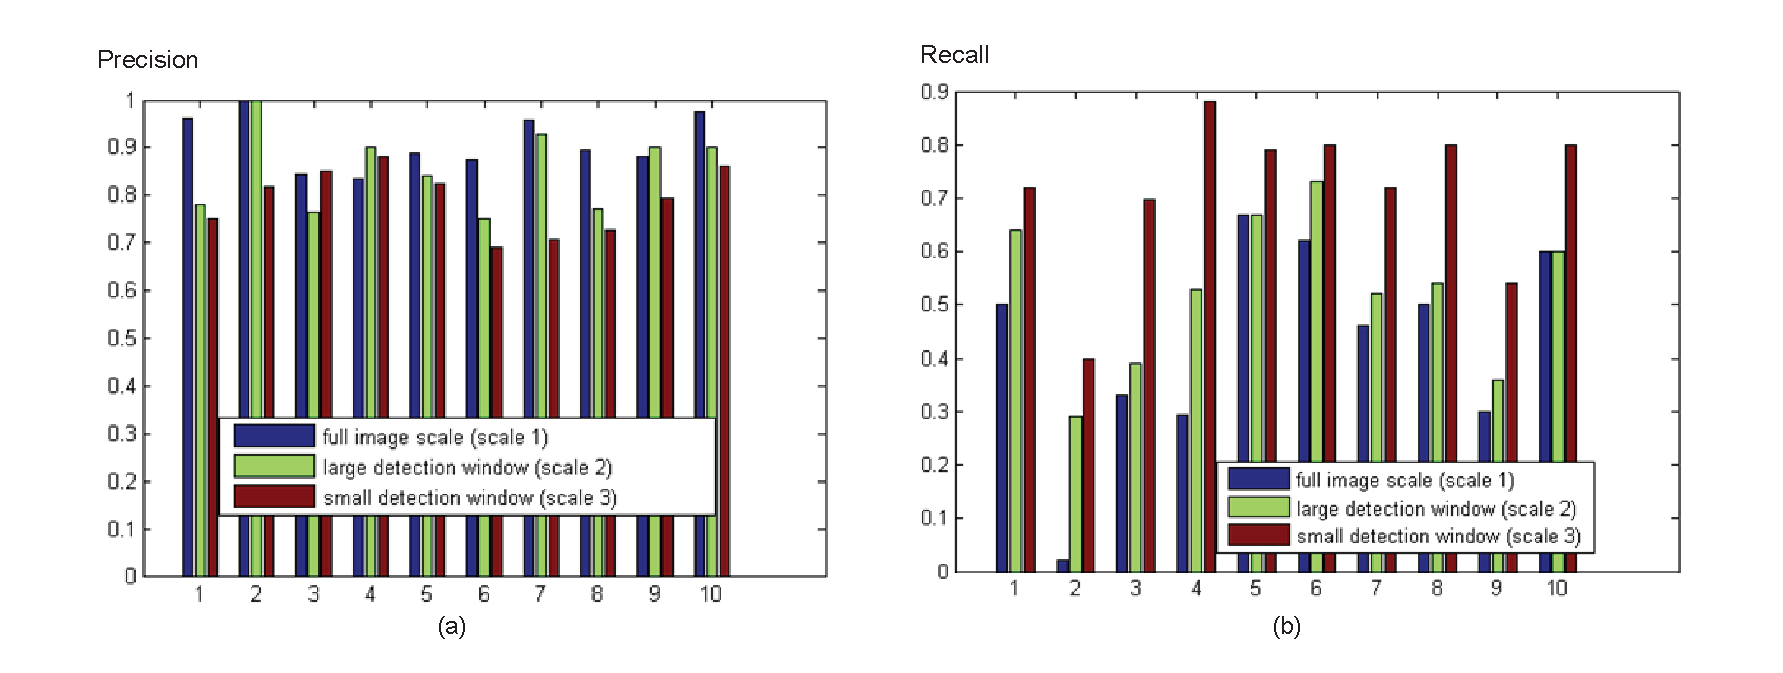
\includegraphics[width=\textwidth]{Chap2_trend}
\vspace {0em}\caption{(A) Trend for decreasing precision in finer scales. (B) Trend for increasing recall in finer scales.}
\label{Chap2_trend}
\vspace {0em}
\end{figure}



Table {\ref{earres}} and {\ref{mouthres}} show the results for ear and mouth/lip disease images. Our method achieved average precisions of
80.7\% and 84.2\%, while the baselines of test set quality were
43.4\% and 47.5\%, respectively. The three evaluation criteria in
table {\ref{earres}} are similar between the two methods ($p>0.1$), and the
average precision of our method for ear disease retrieval was
higher than that of the supervised method. In table \ref{mouthres}, our
method achieved around 6\% average higher precision than the
supervised method ($p=0.15$), at the cost of lower recall. One
possible reason is that the body parts in some mouth disease
images from the test sets are at very different angles and considerably
deformed.
\setlength{\tabcolsep}{5.7pt}
\begin{sidewaystable}
\centering
\caption{Performance Comparison on Ten Ear Disease Image Test Sets.}\label{earres}
\renewcommand{\arraystretch}{1.3}
\begin{tabular}{cccccccc}
\hline
\multicolumn{2}{l}{Ear diseases} & \multicolumn{3}{l}{Object Detection Based Method} &
\multicolumn{3}{l}{Supervised Classification Method} \\ \hline
Disease CUI    &Disease Term & Precision & Recall & F1    & Precision & Recall & F1 \\ \hline
C0008373	&Cholesteatoma&	0.794	&0.818&	0.806&	0.881&	0.953&	0.915\\ \hline
C0013446	&Acquired Ear Deformity&	1.000&	0.828&	0.906&	0.819&	0.863&	0.840\\ \hline
C0013449	&Ear Neoplasms	&0.875	&0.412&	0.560&	0.733	&0.567&	0.639\\ \hline
C0029877	&Ear Inflammation	&0.921&	0.778	&0.843	&0.822	&0.804	&0.813\\ \hline
C0154258	&Gouty tophi of ear	&0.792	&0.655&	0.717&	0.614	&0.470&	0.532\\ \hline
C0347354	&Benign neoplasm of ear	&0.571	&0.533&	0.552&	0.820	&0.497&	0.619\\ \hline
C0423576	&Irritation of ear	&0.733	&0.611	&0.667	&0.933	&0.607	&0.735\\ \hline
C0521833	&Bacterial ear infection&	0.786	&0.647&	0.710&	0.820	&0.670&	0.737\\ \hline
C0729545	&Fungal ear infection	&0.800	&0.696	&0.744&	0.728	&0.864	&0.791\\ \hline
C2350059	&Cancer of Ear&	0.800	&0.414&	0.545&	0.797	&0.699&	0.736\\ \hline
\multicolumn{2}{l}{Average}&0.807&	0.639	&0.705&	0.797	&0.699&	0.736\\ \hline
\end{tabular}
\end{sidewaystable}

\setlength{\tabcolsep}{5.7pt}
\begin{sidewaystable}
\centering
\caption{Performance Comparison on Ten Mouth/Lip Disease Image Test Sets.}\label{mouthres}
\renewcommand{\arraystretch}{1.3}
\begin{tabular}{cccccccc}
\hline
\multicolumn{2}{l}{Mouth/Lip diseases} & \multicolumn{3}{l}{Object Detection Based Method} &
\multicolumn{3}{l}{Supervised Classification Method} \\ \hline
Disease CUI    &Disease Term & Precision & Recall & F1    & Precision & Recall & F1 \\ \hline
C0007971	&Cheilitis	&0.846&	0.667&	0.746	&0.828&	0.893	&0.859\\ \hline
C0019345	&Herpes Labialis&0.900	&0.486	&0.632	&0.817	&0.953&	0.880\\ \hline
C0023761	&Lip Neoplasms	&0.909	&0.500	&0.645	&0.607	&0.553	&0.579\\ \hline
C0149637	&Carcinoma of lip	&0.952	&0.435	&0.597&	0.819	&0.906	&0.860\\ \hline
C0153932	&Benign neoplasm of the lip	&0.625	&0.333	&0.435	&0.833&	0.713	&0.769\\ \hline
C0158670	&Congenital fistula of lip	&0.700	&0.368&	0.483	&0.693	&0.800	&0.743\\ \hline
C0221264	&Cheilosis	&0.750	&0.577	&0.652	&0.813	&0.867	&0.839\\ \hline
C0267022	&Cellulitis of lip	&0.923	&0.600	&0.727	&0.810	&0.917	&0.860\\ \hline
C0267025	&Contact cheilitis	&0.950&	0.543	&0.691	&0.849	&0.943	&0.894\\ \hline
C0267032	&Granuloma of lip	&0.867	&0.500	&0.634&	0.721	&0.865&	0.786\\ \hline
\multicolumn{2}{l}{Average}&0.842	&0.501	&0.624&	0.779&	0.841	&0.807 \\ \hline
\end{tabular}
\end{sidewaystable}

\subsection{Multiple-organ disease classification}
Experiment B evaluated the performance of our method on 220
images of two diseases that are located on multiple organs.
Table {\ref{multiorgan}} shows that the precision of the proposed method on
both test sets was $>80\%$. Compared with the supervised
method, our method improved precision by more than 10\% in
these two cases. Since the proposed method is guided by the
semantic information of body part location, it can detect
various kinds of positive images, whereas the supervised method
does not make use of the high-level features that have greater
semantic meaning.

For hand, foot, and mouth disease, 42.9\%, 28.6\%, and
37.1\% of the positive images in the test set contained a hand,
foot, and mouth, respectively. A few positive images contained
two or three body parts at the same time. The hand, foot, and
lip/mouth detectors contributed to finding 28.6\%, 14.3\%, and
28.6\% of the total positive images. For Ascher's syndrome,
67.9\% and 32.1\% positive test images contained lip and eye,
respectively. The corresponding mouth/lip and eye detectors
found 57.1\% and 28.6\% positive images, respectively, from the
whole test sets.

In summary, we trained five organ detectors and reused them
to filter 2220 web images of 32 different diseases in two experiments.
Compared with the supervised approach that require
training 32 classifiers for each of the diseases, we reduce the
labeling efforts to 15.6\%. The average retrieval precision of our
method on all the 32 datasets was 81.6\%, an improvement of
3.9\% compared with the supervised method. For 13 out of 32
disease datasets, we improved the retrieval precision by 10\%.

\setlength{\tabcolsep}{5.7pt}
\begin{table*}
\centering
\caption{Performance Comparison on Ten Mouth/Lip Disease Image Test Sets.}\label{multiorgan}
\renewcommand{\arraystretch}{1.3}
\begin{tabular}{{lm{3.5cm}m{3.5cm}m{3.5cm}}}
\hline
\multicolumn{2}{l}{Disease CUI} & C001852 &C0339085 \\
\multicolumn{2}{l}{Disease Term} & Hand, Foot and Mouth Disease &Ascher's syndrome \\ \hline
%Positive percentage &0.58 &0.56
\multicolumn{2}{l}{Disease Locations} &C0222224  Skin structure of hand &C0023759 Lip structure\\
\multicolumn{2}{l}{ }&C0222289 Skin structure of foot  &C0015426 Eyelid structure\\
\multicolumn{2}{l}{ }&C0026639 Oral mucous membrane structure& \\
\multicolumn{2}{l}{Detectors} & Hand, Foot and Mouth/Lip &Mouth/Lip and Eye \\
\multicolumn{2}{l}{Positive percentage} & 0.58 &0.56 \\ \hline
\multirow{2}{*}{Precision} &Object detection based     & 0.8333 &0.8889\\
                        &Supervised classification  &0.6944  &0.7857\\
\multirow{2}{*}{Recall} &Object detection based     & 0.7143 &0.8571\\
                        &Supervised classification  &0.7753  &0.9429\\
\multirow{2}{*}{F1} &Object detection based     & 0.7692 &0.8727\\
                        &Supervised classification  &0.7326  &0.8571\\ \hline
\end{tabular}
\end{table*}




\section{Discussion}
With the aim of achieving large-scale medical image retrieval,
we compared the proposed ontology-guided approach with
standard supervised classification. We showed that the proposed
method achieves a precision comparable to that of the supervised
method while saving manual labeling efforts by an order
of magnitude. The results also illustrated that our method has
limitations in low recall values on some test sets and in decreasing
precision when the detection scale becomes smaller. To
improve the recall, we need more robust algorithms and better
data to train the organ detectors. For the limitation of decreasing
precision, we plan to build a two-layer learning model, in
which the first layer classifiers detect target objects at different
scales and the second layer classifier learns the weights to
combine results from the first layer and make final decisions.

The scale of our experiments is limited owing to the intensive
manual labeling work required for training data and evaluation
purposes. Our experiments are based on five organ detectors. In
the future, we plan to train more organ detectors and apply the
method to handle more diseases. We also found that a few
organs, such as skin, muscle, and veins, do not appear as concrete
objects in images. Our method based on object detection
is insufficient for diseases on these organs. In future work, we
plan to add texture pattern recognition to further improve the
retrieving precision and cover a wider range of diseases.

Our approach also depends on disease-organ relationships in
the UMLS, and assumes that the appearance of related organs
determines if the image is disease-related or not disease-related.
Although the assumption is true for many cases as we have
shown, a small number of false-positive samples retrieved by
our method are still non-disease images (only contain normal
organs), or images of a different disease. Another limitation of
this assumption is that the value of ``has\_finding\_site" relationship
in the UMLS is incomplete. Among 74 785 disease concepts
of semantic-type ``disease or syndrome," ``neoplastic
process," ``acquired abnormality," and ``congenital abnormality,"
44.1\% have values in ``has\_finding\_site." For disease terms that
have no body-site information, we plan to extend our approach
by scanning the web images with all organ detectors. In this
way, the ``has\_finding\_site" relationship in the UMLS can be
enriched by mining web images.

\section{Conclusions}
In this work, we developed an ontology-guided disease image
retrieval method based on body-part detection towards mining
web images to build a large-scale health image base for consumers.
Compared with standard supervised classification, the
proposed method improves the retrieval precision of complex
disease images by incorporating semantic information from
medical ontologies. In addition, our method significantly
reduces manual labeling efforts by reusing a set of pretrained
organ detectors. The resulting health image database is annotated
using terms from standard medical ontologies and will
create a rich source of information for multiple descriptive and
educational purposes. Although the scale of our study is limited,
it proves the concept that the web is a feasible source for
automatic health image retrieval, and it only requires a small
amount of manual effort to collect and annotate complex
disease images. In future work, we plan to improve the accuracy
of organ detectors and ontology-based classification, and extend
our approach to handle a wider range of diseases. 
%\chapter{Causal Inference Based Fault Localization for Numerical Software with NUMFL}\label{chap:NUMFL}

NUMFL is a value-based causal inference model for localizing faults in numerical software.  NUMFL combines causal and statistical analyses to characterize the causal effects of individual numerical expressions on output errors.  Given value-profiles for an expression's variables, NUMFL uses generalized propensity scores (GPSs) or covariate balancing propensity scores (CBPSs) to reduce confounding bias caused by evaluation of other, faulty expressions.  It estimates the average failure-causing effect of an expression using quadratic regression models fit within GPS or CBPS subclasses.  We report on an empirical evaluation of NUMFL involving components from four Java numerical libraries, in which it was compared to five alternative statistical fault localization metrics.  The results indicate that NUMFL is the most effective technique overall. We also found that NUMFL works fairly well with data from failing runs alone.

\section{Introduction}\label{introduction}
\vspace{-2pt}
Numerical software plays a very important role in science, industry, and defense, and failures of numerical software have been reported as the cause of several well-publicized ``disasters" \cite{VuikWeb,Kanewala2014}.  However, automated techniques intended specifically for localizing numerical faults based on execution data have received relatively little attention from researchers, although there has been substantial research on general {\it statistical fault localization} (SFL) techniques (e.g. \cite{Jones2002,Liblit2004,Liu2005}) and on other general automated debugging techniques (see Section \ref{relatedwork}).

Typical SFL techniques take data characterizing a set of both passing and failing program executions, including PASS/FAIL labels (provided by testers or end users) and recorded profiles of internal program dynamics, and they compute statistical measures of the strength of the association, if any, between the occurrence of software failures and the occurrence of certain runtime events at particular program locations.  These measures are then used to help guide the search for the causes of observed failures, typically by ranking program statements by the strengths of their associations with failures.  When SFL techniques are evaluated they are generally used as the sole source of information about possible fault locations.  However, it seems more realistic to envision them ultimately being used in combination with other sources of information, such as programmer hunches and {\it fault prediction models} \cite{Fenton1999} based on static code properties and project history.  Potentially, SFL techniques provide a relatively inexpensive way to maximize the information obtained by testing.

 In the vast majority of research on SFL, execution dynamics have been characterized either purely by {\it code-coverage profiles} (also called ``spectra"), indicating which statements, branches, or paths were covered by each execution (e.g., \cite{Jones2002}), or by indicators of the outcomes of {\it predicates} (e.g., \cite{Liblit2004}) – both existing branch predicates and predicates inserted specifically to enhance SFL (e.g., ones that compare the values of numeric variables to zero).  Although the outcomes of such predicates reflect the {\it values} of program variables, they may do so inadequately for SFL, e.g., because predicates or conditions are omitted mistakenly, because they are hidden in library code or microcode, or because few predicates are actually required in the program.  These facts make typical SFL techniques {\it poorly suited} for localizing faults in numerical programs and subprograms having relatively few conditional branches.  Even predicates inserted in a program to enhance SFL are likely to characterize the values of numeric variables inadequately, unless application-specific information is available that indicates which predicates should be inserted.

Although purely numerical programs, and numerical components of other programs, are often relatively small, the intricacy of their computations can make them very difficult to debug manually.  In order to provide automated fault localization assistance to developers who need to debug numerical programs or components, we present a new approach to SFL, denoted by {\it NUMFL}, that is designed specifically to localize faults in numerical code.  NUMFL, like some other recent work on SFL \cite{Baah2010,Baah2011, Gore2012,Shu2013}, is based on {\it causal inference methodology} \cite{Pearl2003}, which seeks to mitigate biases like confounding bias that can badly distort SFL scores used to guide the search for faults.  However, in contrast to previous work, NUMFL is based on generalized forms of {\it propensity scores} \cite{Imai2004,Imai2014}, which are a fairly recent development in causal inference that provide a means of reducing confounding bias when estimating the causal effect of a numeric {\it treatment} or {\it exposure} variable on an outcome variable.

In this chapter, each value of the ``treatment" variable $T_e$ is the result of evaluating a numerical expression or subexpression with a {\it unique program location} identified by $e$,   and the outcome variable $Y$ represents the error (possibly zero) in the output of the numerical program or component under consideration.  The causal effect of $T_e$ on $Y$ is characterized by a function $r_e (t)$, which in medical research is called a {\it dose-response function} (DRF) \cite{Hirano2004}.  To enable localization of faults, NUMFL summarizes the behavior of $r_e (t)$ over a set of evaluations of expression $e$, with a single quantity $susp(e)$ called a {\it suspiciousness score}. It employs generalized propensity scores to make it less likely that a correct expression will receive a high suspiciousness score because it used variables whose values were erroneous due to faults in {\it other} expressions. Note that we do {\it not} use propensity scores themselves as suspiciousness scores; the two kinds of scores have very different purposes.

We assume that (in most cases) users of NUMFL have a set of program or component inputs that induces multiple failing and multiple passing runs.  For these inputs, NUMFL requires corresponding {\it expected outputs} (not just PASS/FAIL labels) and execution profiles characterizing variable values.  The expected outputs are provided by testers or end-users, and the profiles are recorded automatically by program instrumentation.  To compute the suspiciousness score $susp(e)$,  NUMFL requires, in addition to values of the treatment variable $T_e$ and the output-error variable $Y$, corresponding values of the set of variables {\it used} in expression $e$.  Although the value-profiles used by NUMFL are more detailed than basic coverage profiles used by typical SFL techniques, the potential cost of recording and analyzing value profiles is offset by the relatively small size of many numerical programs.   Moreover, we assume that developer-time is a more critical resource in debugging than is computation time, because developers usually can do other work while an SFL algorithm runs.

The main contributions of this chapter are:
\vspace{-0.2cm}
\begin{itemize}
\item NUMFL, a new, value-based approach to SFL for numerical programs, which is based on sound causal inference methodology
	\item A new, value-based approach to SFL for numerical programs, named NUMFL, that is based on sound causal inference methodology, and two variants of NUML, denoted NUMFL-GPS and NUMFL-CBPS, based on alternative forms of generalized propensity scores
	\item The first use of generalized propensity scores to reduce confounding bias in SFL
	\item An implemented platform to profile the variables used and defined by numerical expressions in Java programs
\item An empirical comparison of NUMFL to five competing SFL techniques on components from four widely-used Java numerical libraries, which indicates that NUMFL is more effective overall than the other techniques
    \item Empirical evaluations of NUMFL on programs with single faults, with multiple faults, with both passing and failing executions, and with only failing executions
\item	An empirical comparison of NUMFL-GPS and NUMFL-CBPS to each other
\end{itemize}

This chapter is a revised and extended version of \cite{Bai2015}, which presented NUMFL-GPS, but not NUMFL-CBPS, and which evaluated NUMFL-GPS on only single-fault programs and with a mixture of passing and failing executions. The rest of the chapter is organized as follows: we present a motivating example in Section \ref{motivating}; background for our approach is presented in Section \ref{background}; NUMFL is described in detail in Section \ref{twoversion};  we report on its empirical evaluation in Section \ref{evaluation}; related work is surveyed in Section \ref{relatedwork}; and Section \ref{conclusion} concludes the chapter.

\section{Motivating Example}\label{motivating}

Figure \ref{code} shows a short function {\it harmean}, which correctly calculates the harmonic mean of two floating point numbers, in the middle column and shows a faulty version of {\it harmean} in the rightmost column.  (In real fault localization scenarios only the faulty code is usually available.)  We injected a fault into statement $s_3$ by adding a floating point number $c$ to the original expression $a*b$.  Given a pair of inputs $(a,b)$, the faulty version of $s_3$ produces an erroneous value for the variable $x$.  This value may propagate to statement $s_8$ and, via the variable $r$, cause an incorrect return value at statement $s_9$.  We use $r_{correct}$ and $r_{faulty}$ to denote the return value of the correct code and faulty code, respectively.  Let us assume that the faulty version of {\it harmean}, like many numerical programs, is considered to fail if the output error exceeds a predefined threshold $\epsilon$, that is, if

\begin{equation*}\label{threshold}
outerr = |{r_{correct}} - {r_{faulty}}| > \varepsilon
\end{equation*}

\begin{figure*}[!thpb]
\centering
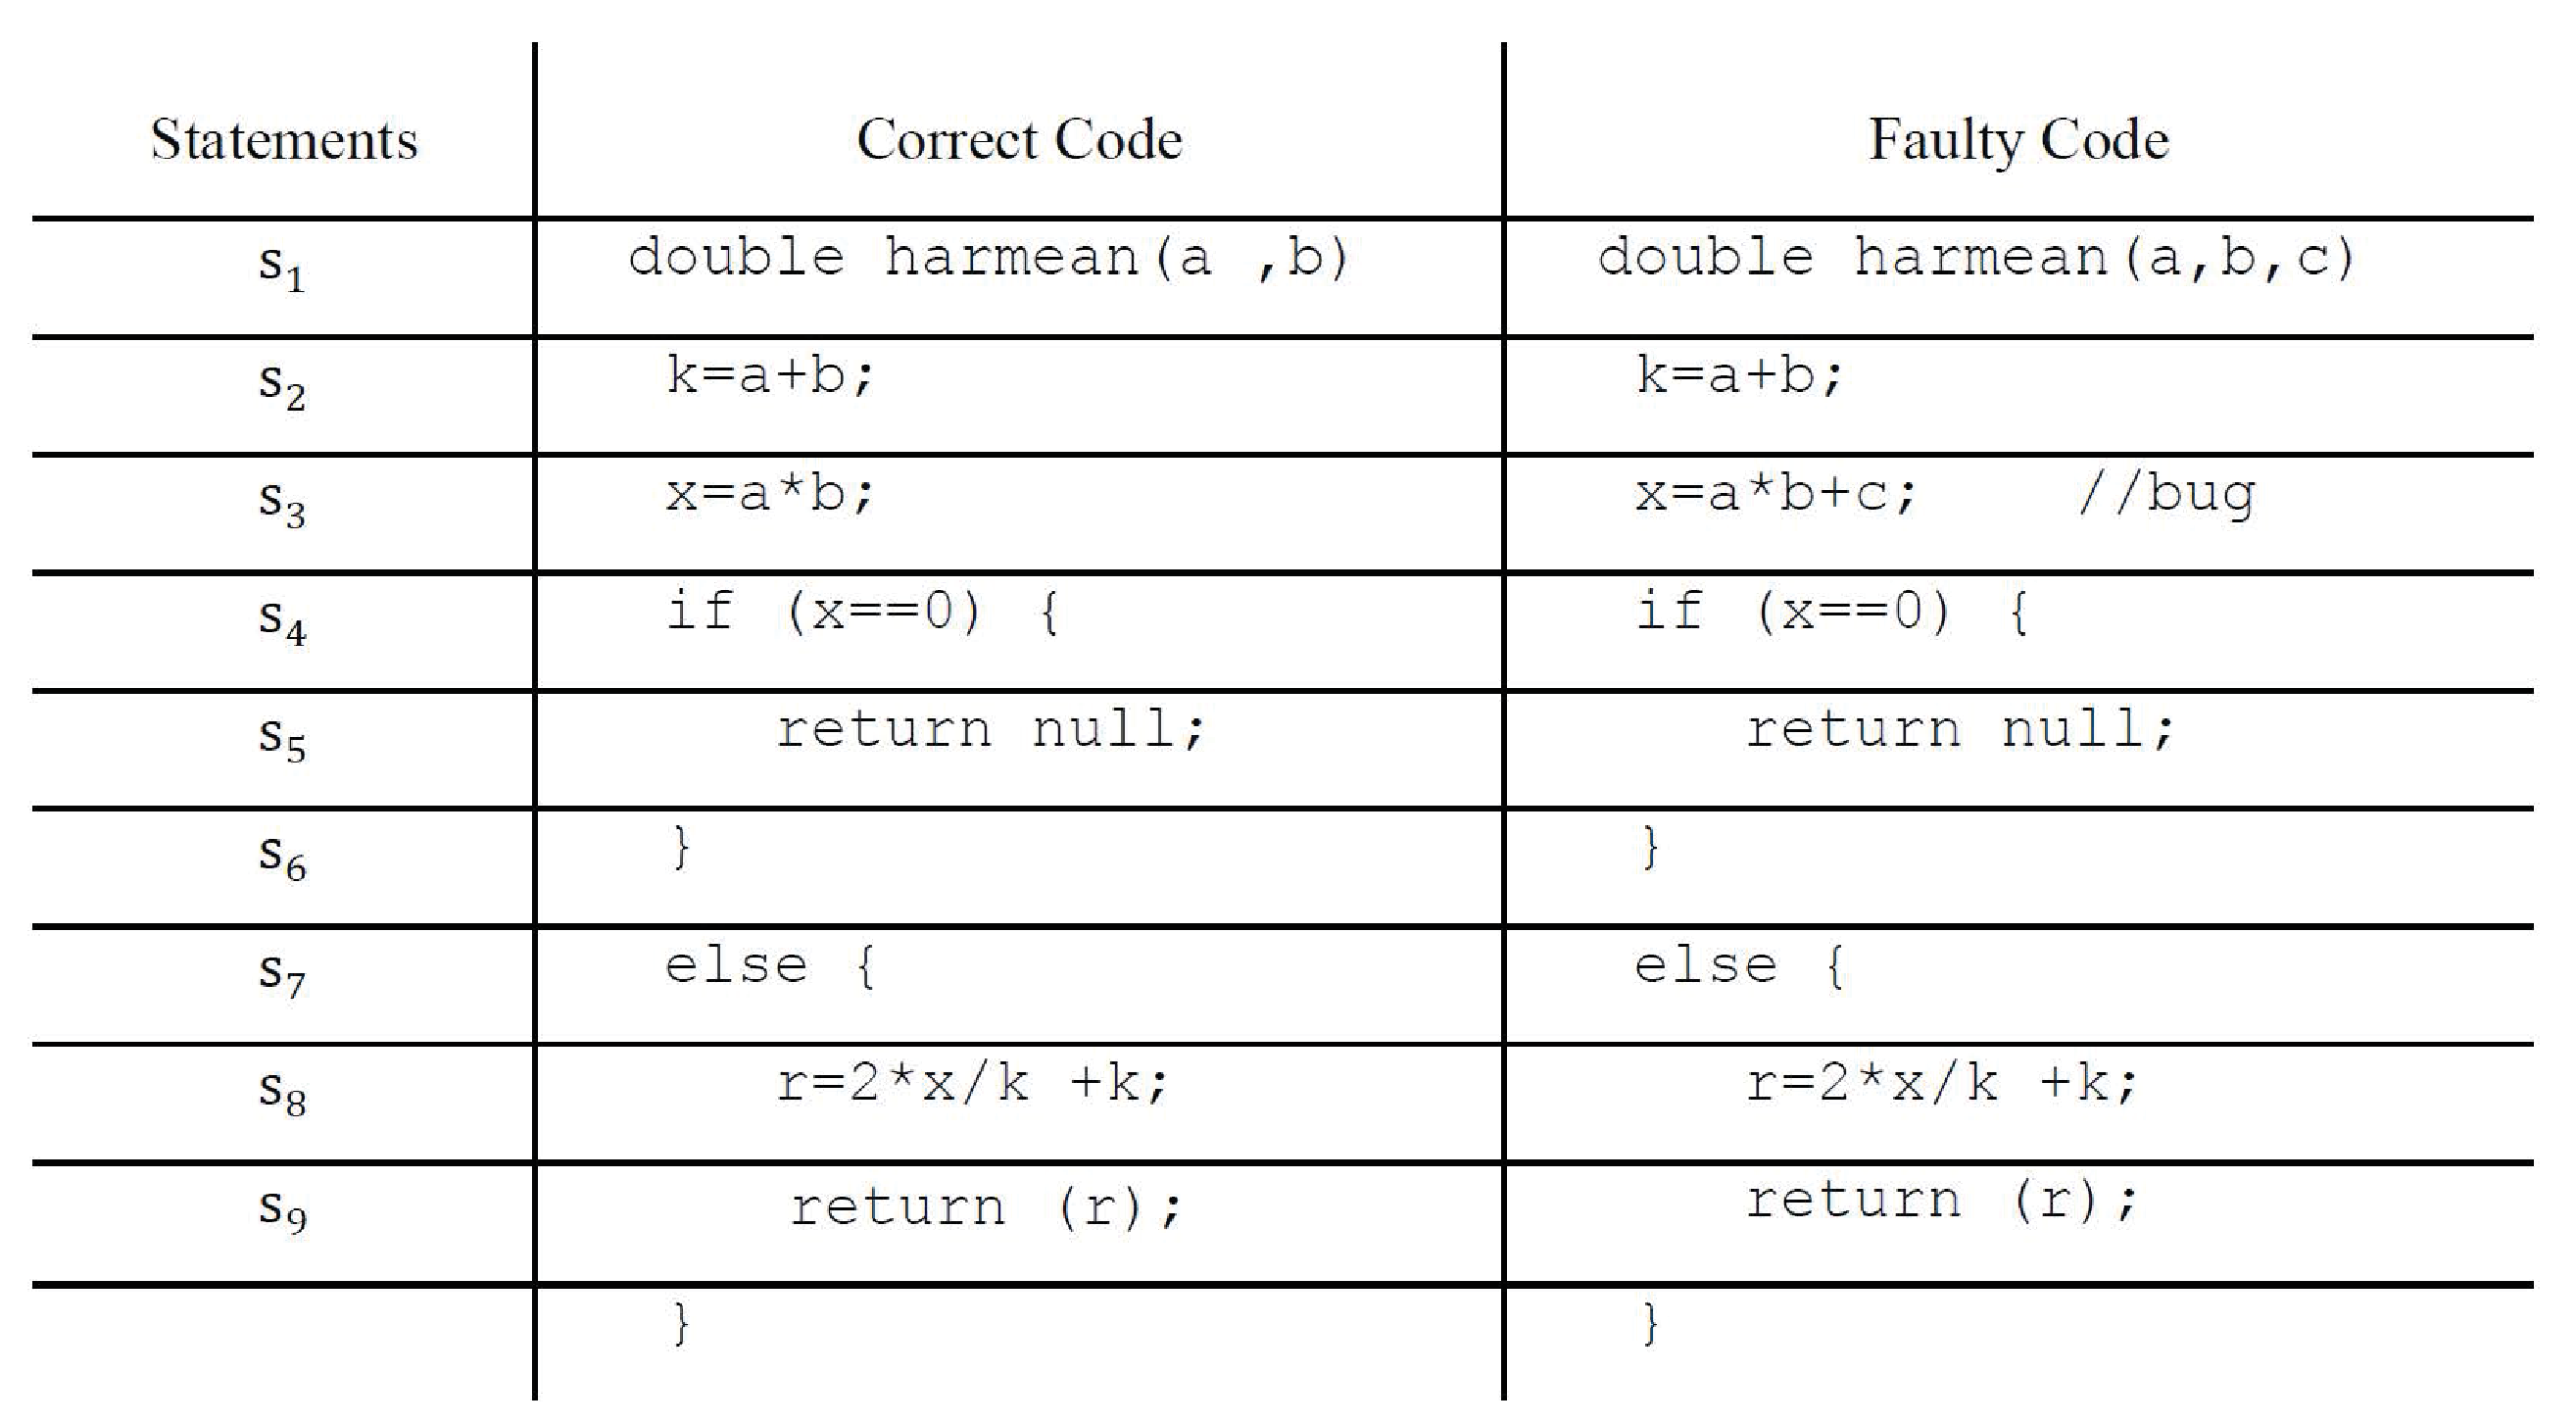
\includegraphics[width=0.8\textwidth]{MotivatingExample.eps}
\caption{Motivating Example}
\label{code}
\end{figure*}

Our goal is to automatically localize faults in numerical expressions, given variable-value profiles and expected outputs.  In the faulty code of Figure \ref{code}, there are three numerical expressions, in statements $s_2$, $s_3$ and $s_8$ , which define variables $k$, $ x$, and $r$.  A simple approach to detecting which expressions contain numerical faults is to obtain a ``suspiciousness" score for each numerical expression by calculating a measure of the statistical association between the values of the expression and the output error. This na\"{i}ve approach has two potential problems, however.  First, erroneous values due to a fault in one expression may propagate to other, correct expressions, causing them to receive high suspiciousness scores.  For example, in Figure \ref{code} the fault in statement $s_3$ causes variable $x$ to have erroneous values that propagate to statement $s_8$ and cause variable $r$ to have erroneous values. Consequently, the output error of {\it harmean} is associated with the values computed by both $s_3$ and $s_8$, even though $s_8$  is correct.  This problem, which is an instance of {\it confounding bias} (or {\it confounding}), is due to the fact that the computation of $x$ at $s_3$ is a {\it common cause} of program failure and of the computation of $r$ at $s_8$.  A na\"{i}ve measure of the association of $r$ with the output error, which does not account for confounding, will reflect both the true causal effect of $r$ on failure and the biasing effect of the confounder $x$ on $r$ and $outerr$.

The second problem with the na\"{i}ve approach is that common association measures like Pearson's correlation coefficient \cite{Philip2012} are often inadequate to measure the causal effect of a numerical expression on a program's output error, even without confounding.  For the example in Figure \ref{code},  $outerr=|r_{correct}-r_{faulty} |=|2c/(a+b)|$.  If $a=1$ and $b=0$, then $outerr=2|c|$ and $x=c$.  By definition, the correlation between $x$ and $outerr$ is:
\begin{equation*}\label{correlation}
%corr(x,outerr) = \frac{{{\mathop{\rm cov}} (x,outerr)}}{{{\sigma _x}{\sigma _{outerr}}}} = \frac{{{\mathop{\rm cov}} (c,2|c|)}}{{{\sigma _x}{\sigma _{outerr}}}}
corr(x,outerr) = \frac{{{\mathop{ cov}} (x,outerr)}}{{{\sigma _x}{\sigma _{outerr}}}} = \frac{{{\mathop{ cov}} (c,2|c|)}}{{{\sigma _x}{\sigma _{outerr}}}}
\end{equation*}
where $cov(x,outerr)$ is the covariance between $x$ and $outerr$ and where $\sigma_x$ and $\sigma_{outerr}$ are the standard deviations of $x$ and $outerr$, respectively.  Using basic covariance identities, we find that $cov(c,2|c|)=2cov(c,|c|)=2E[(c-\mu_c )(|c|-\mu_{|c|})]$, where $\mu_c$ and $\mu_{|c|}$ are the means of $c$ and $|c|$ respectively.  If the distribution of variable $c$ is symmetric about 0, $cov(c,|c|)$ is equal to 0, and so is $corr(x,outerr)$. Therefore, $corr(x,outerr)$ can be 0, even though the statement defining $x$ contains a fault.

NUMFL is intended to address the aforementioned problems and to provide less-biased estimates of the {\it failure-causing effect} of a numerical expression.  We now map the causal variables defined in the Introduction to the variables in our example:
\begin{enumerate}
\item 	Treatment variable $T_e$ is the variable defined in a numerical expression $e$.  In Figure \ref{code}, variables $k$, $x$ and $r$ are the treatment variables associated with statements $s_2$, $s_3$ and $s_8$, respectively.
	\item Outcome variable $Y$ is the absolute difference between the output of the faulty program and the expected (correct) output.  For the example, $Y$ is $outerr$.
\item $X$ represents the confounding variables, which are each causes of both treatment $T_e$ and outcome $Y$. For example, in the numerical expression $r=2*x/k$, the variables $x$ and $k$ are confounders because they each influence the values of both the treatment $T_e=r$ and the outcome $Y=outerr$.

\end{enumerate}

Figure \ref{dag1} shows the causal relationships between treatment, outcome, and confounding variables.
\begin{figure*}[!thpb]
\centering
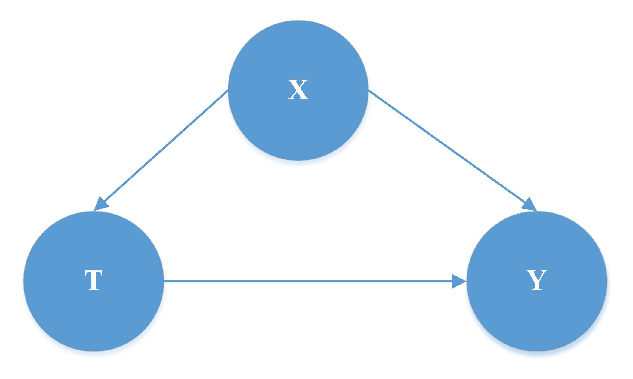
\includegraphics[width=0.5\textwidth]{CausalDAG1.eps}
\caption{Causal diagram of treatment, outcome, and confounder.}
%\vspace{-.5cm}
\label{dag1}
\end{figure*}


\section{BACKGROUND}\label{background}
\subsection{Causal Inference Methodology}\label{IIIA}
Causal inference methodology \cite{Pearl2003} has emerged in recent decades from research in a number of applied fields, to provide a basis for making valid inferences, from experimental or observational data, about the causal effects of specified treatments or exposures upon outcomes of interest.  Data about study variables is augmented with background knowledge about the causal relationships among variables, which is represented as {\it causal DAG}: a directed acyclic graph, in which nodes correspond to variables and in which there is an edge $A \to B$ if $A$ is an actual or assumed cause of $B$.  Causal inference theory establishes graph-theoretic conditions, such as Pearl's Backdoor Criterion \cite{Pearl2003}, under which a given causal effect can be estimated statistically without confounding or other forms of bias such as selection bias and measurement bias.



\subsection{Ordinary Propensity Scores}\label{IIIB}
Consider a treatment variable $T$ with two possible values 1 and 0.  (These values may indicate ``treated" and ``untreated", respectively, or they may indicate alternative treatments.)  One of the reasons that ideal randomized experiments, when they are feasible, are often considered the ``gold standard" for the design of causal inference studies \cite{Grossman2005} is that randomization makes it likely that the joint distribution of the covariates of the units with $T=1$ is similar to the covariate distribution of the units with $T=0$.  Such similarity, which is called {\it covariate balance} \cite{Rosenbaum1983}, implies that the two groups of units are comparable with respect to the values of confounding covariates, so that any difference in average outcomes of the groups is likely to be due to the treatment variable and not to confounding.  In randomized experiments, covariate balance is a consequence of the fact that the randomized treatment variable is {\it independent} of the covariates.

\begin{figure*}[!thpb]
\centering
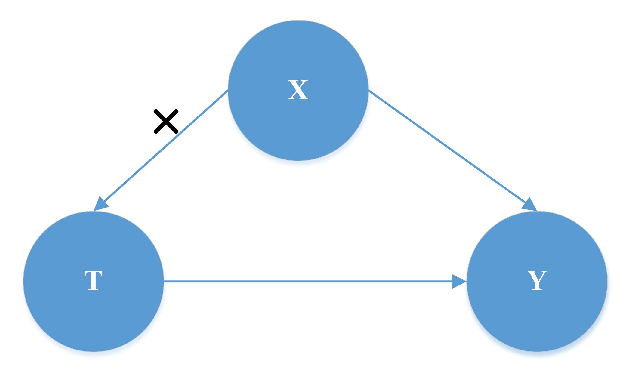
\includegraphics[width=0.5\textwidth]{CausalDAG2.eps}
\caption{Matching units based on their propensity scores breaks the link between cofounding variables and treatment.}
%\vspace{-.5cm}
\label{dag2}
\end{figure*}

An important approach to achieving covariate balance in observational studies is the use of (ordinary) {\it propensity scores} \cite{Rosenbaum1983}.  For a binary treatment variable $T$ and a vector of covariates $\pmb{X}$, the propensity score $Pr(T=1|\pmb{X}=\pmb{x})$ is the conditional probability of treatment $T=1$ given that the observed value of $\pmb{X}$ is $\pmb{x}$.  It has been shown that the propensity score is a {\it balancing score} in the sense that comparison groups with similar propensity scores tend to have similar covariate distributions \cite{Rosenbaum1983}.  True propensity scores are generally unknown, but they can be estimated from data about study units' actual treatment and covariate values.

Suppose that for each unit $i$ examined in an observational study, we have recorded the values of a binary treatment variable ${T_i} \in \{ 0,1\} $ and a vector of covariates ${\pmb{X}_i}$ .  We can use a parametric model ${\pi _{\pmb\beta} }({\pmb{X}_i})$ to estimate the propensity score for unit $i$.  One choice is the logistic model:

\begin{equation*}
{\pi _{\pmb\beta} }({X_i}) = Pr({T_i} = 1|{\pmb{X}_i}) = \frac{{\exp ({\pmb{X}_i}^\prime \pmb\beta )}}{{1 + \exp ({\pmb{X}_i}^\prime \pmb\beta )}}
\end{equation*}

We can estimate the parameter $\pmb\beta$ using maximum likelihood estimation \cite{Silvapulle1981}, which involves maximizing the log-likelihood function:

\begin{equation}\label{eq1}
{\pmb{\hat \beta} _{MLE}} = \arg \;\max \sum\limits_{i = 1}^N {{T_i}\log \left\{ {{\pi _{\pmb\beta} }({\pmb{X}_i})} \right\} + (1 - {T_i})} \log \left\{ {1 - {\pi _{\pmb\beta} }({\pmb{X}_i})} \right\}
\end{equation}

With the fitted model, we can estimate the ordinary propensity score  ${\pi _{\pmb\beta}}({\pmb{X}_i})$ for each observed unit.

After the propensity score model is estimated, covariate balance may be achieved by matching units based on their estimated propensity scores \cite{Rosenbaum1983}.  For example, each unit with $T=1$ can be matched to a unit with $T=0$ that has a similar estimated propensity score, if such a unit exists.  As illustrated in Figure \ref{dag2}, matching units based on their propensity scores breaks the link between the confounding variables and the treatment variable.

Ordinary propensity scores are not applicable to continuous treatment variables, however.  To address confounding of SFL scores for numerical expressions, we consider two variants of ordinary propensity scores that can accommodate continuous (and integer) treatment variables.  The first variant is the Generalized Propensity Score (GPS) proposed by Imai and Van Dyk \cite{Imai2004}.  The second variant is the Covariate Balancing Propensity Score (CBPS) proposed by Imai and Ratkovic \cite{Imai2014}.  Since CBPS is quite new, it has not been established whether it is superior to GPS.  Hence, we shall present and evaluate two versions of NUMFL, denoted NUMFL-GPS and NUMFL-CBPS, which are based on GPS and CBPS, respectively.  First, though, we briefly describe GPS and CBPS in the next two subsections.

\subsection{Generalized Propensity Score (GPS)}\label{IIIC}
The {\it Generalized Propensity Score} proposed by Imai and van Dyk \cite{Imai2004} is intended for use with any kind of treatment variable, including continuous ones.  Let ${p_{\pmb{\psi}} }(T|\pmb{X})$  be a model, with parameters $\pmb{\psi}$, of the {\it conditional probability density function} (p.d.f.) of the treatment variable $T$ given the covariate vector $\pmb{X}$.  The GPS for a specific unit with treatment level $T=t$ and covariate values $\pmb{X=x}$ is the density value $r = {p_{\pmb\psi} }(T = t|{\pmb X} = {\pmb x})$.  Imai and van Dyk \cite{Imai2004} require that the model ${p_{\pmb{\psi}} }(T|\pmb{X})$ has a {\it unique parameter} ${\pmb\theta}  = \pmb{\theta _\psi }(X)$ such that ${p_{\pmb{\psi}} }(T|\pmb{X})$ {\it depends on} $\pmb X$ {\it only through} $\pmb \theta$.  For example, if the treatment is represented by a {\it linear Gaussian model} $T|\pmb{X} \sim {\cal N}(\pmb{X}'{\pmb \beta} ,{\sigma ^2})$ with mean $\pmb{X}'{\pmb \beta}$  (the scalar product $\pmb{X}$-transpose times $\pmb{\beta}$) and variance $\sigma ^2$, so that $\pmb{\psi}  = \left( {\pmb{\beta} ,{\sigma ^2}} \right)$, then $\pmb{\theta}  = \pmb{X}'\pmb{\beta} $ (here $\pmb{\theta} $ is scalar).  The model parameters $\pmb{\psi}$, $r$, $\pmb{\theta}$, $\pmb{\beta}$, etc. are estimated from data; the corresponding estimates are denoted with by $\hat {\pmb\psi} $, $\hat r$, $\hat{ \pmb{\theta}} $, $\hat{ \pmb{\beta}}$, etc..  In Imai and van Dyk's approach, it is the values of the parameter estimate ${{\hat{\pmb{\theta}} }_{\hat{ \pmb{\psi}} }}(\pmb{X})$ that are used to control confounding, rather than the values of ${p_{\hat{ \pmb{\psi}} }}(T|\pmb{X})$ themselves.

Table \ref{exampledata} lists 10 test cases of faulty code in the motivating example. The three inputs $a$, $b$ and $c$ are generated randomly in the range $[-5, 5]$.  Table \ref{exampledata} also shows the values of intermediate variables values of $k$ and $x$ which are defined in expressions $s_2$ and $s_3$ respectively. The variable $r$ in expression $s_8$ is the faulty code's output and the variable $r_c$ represents the output of the correct code in motivating example with the same inputs. Outcome variable $Y$ is equal to $|r-r_c|$, so all the values of $Y$ are positive in the table. All the values in the table are rounding to three decimals. We use expression $s_8$ as an example to demonstrate generalized propensity score is estimated. For expression $s_8$, the treatment variable $T_e$ is variable $r$ and the confounding variables $\pmb{X}$ are covariates $x$ amd $k$. We first fit a linear regression model $T_e = \beta_0+{\beta_1}x+{\beta_2}k$ with $r $ as response, $x$ and $k$ as predictors. Given the data in Table \ref{exampledata}, the fitted regression model is $ T_e =0.614x+1.212k-1.462$. Then we estimate GPS ${{\hat{\pmb{\theta}} }_{\hat{ \pmb{\psi}} }}(x, k)$  by inputting observed value of $x$ and $k$ into the fitted regression model.  The estimated GPS for expression $s_8$ is denoted by$ {\hat{\theta}}_{s_8} $and is shown in the last column of the table.  

The confounding variables' effect on treatment variable can be controlled if conditioned on GPS. This can be proved with the data in Table\ref{exampledata}. For the confounding variable $x$'s effect on treatment variable $r$, we fit two regression models: the first model uses $r$ as respond and $x$ as predictor; the second model uses $r$ as respond, but uses both $x$ and GPS ${\hat{\theta}}_{s_8}$ as predictors. Given the data in Table\ref{exampledata}, the first model is fitted as $ r =0.487x-1.729$ and the second model is fitted as $r=-2.271E^{-16}x+ 1.0{\hat{\theta}}_{s_8}-1.461$. In the first model, the coefficient of $x$ means the variable $r$ will increase 0.487 if $x$ increased 1 unit. In the second model, the coefficient of $x$ is close to 0, while the coefficient of propensity score ${\hat{\theta}}_{s_8}$ is 1. This means the variable value of $r$ is mostly depend on the value of  ${\hat{\theta}}_{s_8}$. Similarly, we can have another two fitted model for the other confounding variable $k$: $r=0.999k-1.415$  and $r=-2.755E^{-16}k+1.0{\hat{\theta}}_{s_8}$-1.461.  The coefficient of $k$ is also reduced to 0 in the second model.  Thus, given GPS, the effect of confounding variables on treatment variable is significantly reduced, which can also be illustrated by Figure \ref{dag2}

\begin{table*}[htbp!]
\caption{VARIABLE VALUES AND GPS OF THE MOTIVATING EXAMPLE}
\label{exampledata}
\centering
      \begin{tabular}{|l|c|c|c|c|c|c|c|c|c|c|}
      \hline
Test \#	&1	&2&3&4 & 5 &6& 7 & 8 & 9&10\\	\hline

$a$ &-1.697	&	4.088	&	0.242	&	-0.269	&	-3.495	&	-2.081	&	-2.063	&	-2.896	&	3.839	&	-3.412 \\ 	\hline
$b$ & -1.430	&	0.660	&	4.843	&	-1.803	&	-3.352	&	1.282	&	-1.520	&	4.568	&	1.796	&	0.325\\	\hline
$c$ & -3.990	&	3.778	&	-2.242	&	-0.347	&	-1.678	&	-0.358	&	3.766	&	-4.690	&	-2.535	&	-1.645 \\	\hline
$k$ & -3.127	&	4.748	&	5.084	&	-2.072	&	-6.847	&	-0.799	&	-3.583	&	1.672	&	5.636	&	-3.088\\	\hline
$x$ &-1.564	&	6.478	&	-1.071	&	0.138	&	10.036	&	-3.025	&	6.902	&	-17.919	&	4.362	&	-2.752 \\	\hline
$r $& -2.127	&	7.477	&	4.663	&	-2.205	&	-9.778	&	6.777	&	-7.436	&	-19.768	&	7.184	&	-1.305\\	\hline
$r_c$ & -4.679	&	5.885	&	5.545	&	-2.540	&	-10.268	&	5.881	&	-5.334	&	-14.157	&	8.083	&	-2.371 \\	\hline
$Y$ & 2.552	&	1.592	&	0.882	&	0.335	&	0.490	&	0.896	&	2.102	&	5.611	&	0.900	&	1.065 \\	\hline
${\hat{\theta}}_{s_8}$ & -4.749	&	9.731	&	5.502	&	-2.426	&	-2.132	&	-2.825	&	-0.102	&	-8.978	&	9.506	&	-5.431\\	\hline

\end{tabular}
\end{table*}


\subsection{Covariate Balancing Propensity Score (CBPS)}\label{IIID}
Section \ref{IIIB} explained that the ordinary propensity score is a balancing score and that it can be estimated from data using a parametric statistical model.  However, if the propensity score model ${\pi _{\pmb \beta} }({\pmb{X}_i})$  is {\it misspecified}, matching on the estimated propensity scores (and related techniques) may fail to balance the covariates, yielding biased estimates of causal effects. To address this problem, Imai and Ratkovic proposed the {\it Covariate Balancing Propensity Score} (CBPS), which is robust to mild misspecification of the propensity score model \cite{Imai2014}.
The CBPS optimizes covariate balance by modifying the estimation procedure for parameter $\pmb{\beta}$ .  Differentiating equation \eqref{eq1}, equating the result to zero, and taking expectations, we have \cite{Imai2014}
\begin{equation}\label{eq2}
E\left\{ {\frac{{{T_i}{{\pi '}_{\pmb \beta} }({\pmb{X}_i})}}{{{\pi _{\pmb \beta} }({\pmb{X}_i})}} - \frac{{(1 - {T_i}){{\pi '}_{\pmb \beta} }({\pmb{X}_i})}}{{1 - {\pi _{\pmb \beta} }({\pmb{X}_i})}}} \right\} = 0,
\end{equation}
where ${\pi '_{\pmb \beta} }({\pmb{X}_i}) = \partial {\pi _{\pmb \beta} }({\pmb{X}_i})/\partial \pmb{\beta}$.  Equation \eqref{eq2} is called a {\it balancing condition} or a {\it moment condition} \cite{Imai2014}.  (The mean of a random variable is its ``first moment" \cite{Rosenblueth1981}.)  In CBPS, the balancing condition is generalized as
\begin{equation}\label{eq3}
E\left\{ {\frac{{{T_i}{{\tilde {\pmb X}}_i}}}{{{\pi _{\pmb \beta} }({\pmb{X}_i})}} - \frac{{(1 - {T_i}){{\tilde {\pmb X}}_i}}}{{1 - {\pi _{\pmb \beta} }({\pmb{X}_i})}}} \right\} = 0,
\end{equation}
where ${\tilde {\pmb X}_i} = f({\pmb{X}_i})$ represents a vector-valued function of the covariates $\pmb{X}_i$. To ensure that the first moment of each covariate is balanced, even when the model is misspecified, we can set ${\tilde {\pmb X}_i} = {\pmb{X}_i}$. CBPS employs a parameter estimation framework called the {\it generalized method of moments} (GMM) \cite{Hansen1982}, which is based on solving moment-condition equations for the parameters of interest and substituting sample moments for unknown population moments. Imai {\it et al}. extended CBPS to treatments with $K>2$ integer values, using a $multinomial\;model$ for the conditional probability of treatment given the covariates. We adapted this approach slightly to make it applicable to value-based fault localization (see Section \ref{IVB}), and we evaluate CBPS in NUMFL as an alternative to GPS .

\section{TWO VERSIONS OF NUMFL}\label{twoversion}
In this section, we define two versions of NUMFL, NUMFL-GPS and NUMFL-CBPS, and explain how they are used to reduce confounding bias during estimation of a numerical expression's {\it average failure-causing effect} (AFCE). Intuitively, an aggregate measure of the failure-causing effect of a numerical expression $e$ should summarize the effects on output errors of evaluating $e$ over a sample of program runs that each cover or reach $e$. Accordingly, in causal inference the designated ``treatment" variable $T_e$ should reflect the values produced by individual evaluations of $e$. (Of course $e$ may be evaluated repeatedly in a single program run, due to iteration.) Runs that do not reach $e$ are {\it not relevant} to such a measure. This is unlike measures of the failure-causing effect of covering a statement $s$ at least once during a run (e.g., \cite{Jones2002}), which contrast runs that cover $s$ with runs that don't cover $s$. With such measures, the treatment variable indicates whether or not $s$ was covered during a given run.

Recall that confounding of the causal effect of a treatment variable $T$ upon an outcome variable $Y$ is bias that is due to the presence of one or more common causes of $T$ and $Y$. The influence of such a common cause $X$ can make the effect of $T$ on $Y$, as reflected by a na\"{i}ve measure of statistical association, appear to be stronger or weaker than it really is. As mentioned in Section \ref{IIIB}, ordinary propensity scores cannot be used in causal inference to control confounding when the treatment variable is continuous.  Since the ``treatments" that NUMFL deals with are the values of numeric program variables, we instead define and evaluate two versions of NUMFL, namely NUMFL-GPS and NUMFL-CBPS, that are based respectively on GPS and CBPS, the two generalizations of ordinary propensity scores described in Sections \ref{IIIC} and \ref{IIID}.

\subsection{NUMFL-GPS}\label{IVA}
As with ordinary propensity scores, GPS is used to control for statistical associations between the treatment variable and confounding covariates, which in the case of NUMFL are variables used (read) in a numeric expression $e$ whose AFCE we wish to estimate. In general, these program variables are potential confounders because they may contain erroneous values just before expression $e$ is evaluated, due to faults in previously evaluated expressions. If these erroneous values cause program failures (that is, ``coincidental correctness" does not occur) the result of evaluating $e$ may be strongly associated with failures even if $e$ is correct, unless steps are taken to control confounding. In NUMFL, therefore, when estimating the AFCE of $T_e$ on the output error $Y$, we control for the values of the variables used in $e$.  (Those familiar with Pearl's Backdoor Adjustment Criterion \cite{Pearl2003} should note that this breaks any backdoor paths between $T_e$ and $Y$ in the acyclic data flow graph induced by a program execution.)

\subsubsection{Control of Confounding.}
For a given numerical expression $e$ in a program, NUMFL-GPS currently fits a linear
Gaussian GPS model ${{\pmb T}_e}|{{\pmb X}_e} \sim N({\pmb X}_e'{{\pmb \beta} _e}, \sigma _e^2)$ , where the treatment variable $T_e$ represents the result of evaluating $e$ (once) and where the possibly confounding covariates in the vector $\pmb{X}_e$ represent the corresponding values of the program variables used in evaluating $e$. Observe that one program run may generate multiple values of $T_e$ and $\pmb{X}_e$, due to iteration. To reduce profiling overhead, these may be sampled rather than recorded exhaustively. We currently sample only the values from the {\it last iteration} of a loop.

Applying GPS in NUMFL entails the following three steps:
\begin{enumerate}
\item 	Given a sample of observed values for the treatment variable $T_e$ and for the covariates $\pmb{X}_e$, fit a linear regression model $T_e=\pmb{X}_e' \pmb{\beta}_e$ to obtain the estimated parameter vector $\hat {\pmb{\beta}}_e$.
\item For each observed value ${\pmb x}_{e,i}$ of $\pmb{X}_e$, compute the estimate ${{\hat \theta }_{e,i}} = {\pmb{x}_{e,i}}'{{\hat {\pmb{\beta}} }_e}$.
\item Group observations with the same or similar values of $\hat{\theta}_{e,i}$ into $m$ subclasses of roughly equal size.
\end{enumerate}

The regression model fitted in the first step characterizes how the values of the covariates in $\pmb{X}_e$ influence the value of the treatment variable $T_e$.  In the second step, $\hat{\theta}_{e,i}$ estimates this influence for a particular value $\pmb{x}_{e,i}$ of $\pmb{X}_e$.  The scalar $\hat{\theta}_{e,i}$ summarizes the influence of the vector value $\pmb{x}_{e,i}$ on the treatment, and hence $\hat{\theta}_{e,i}$ may be used in place of $\pmb{x}_{e,i}$ for confounding control. Accordingly, in the third step, each subclass of observations with similar $\hat{\theta}_{e,i}$ values corresponds to a set of $\pmb{x}_{e,i}$ values that influence the treatment similarly. Thus, within each subclass, there is little or no association between confounders and the treatment variable $T_e$.

To illustrate this procedure, we refer again to the faulty version of the function {\it harmean} in Figure \ref{code}.  Statement $s_8$ is $r=2*x/k +k$. To control possible confounding of the average failure-causing effect of $r$ by the variables $x$ and $k$, we first fit a linear model $r=\beta_1 z+\beta_2 k$, where $z=x/k$, using a sample of corresponding observed values $(r_i,x_i,k_i)$. Second, we apply the fitted model to each pair $(x_i,k_i)$ to obtain a predicted value $\hat \theta_i$.  Third, we group the observations with similar $\hat \theta_i$ values into subclasses. This can be done by sorting the $\hat \theta_i$ into descending order and partitioning the sorted values into $m$ roughly equal-size bins.

Although GPS can control confounding bias caused by multiple confounding covariates, there is one challenge to applying it in NUMFL-GPS. If the dimension of $\pmb{X}_e$ is high, the first step of GPS requires a large number of observations to fit a suitable regression model.  In practice, a numerical expression defined by a statement could contain more than 10 confounders, but the number of tests may not be large enough to fit the regression parameters with adequate precision. Thus, to apply GPS, we need to control the dimension of confounding variables.

To address this problem, we $decompose$ a complex numerical expression into several subexpressions, each involving operators with the same precedence level.  For example, a numerical statement $a=(b+c+d)*e$ will be decomposed into two subexpressions: (1) $temp=b+c+d$ and (2) $a=temp*e$.  Here, $temp$ is a temporary variable that plays the role of the treatment variable for subexpression (1) and the role of a possible confounder for subexpression (2). Thus, each subexpression has fewer confounding variables and a relatively simple structure.  For each subexpression, we use GPS to control confounding bias and then estimate the subexpression's AFCE.

\subsubsection{Failure-causing Effect Estimation.}
Within each of the subclasses created by grouping observations with similar $\hat \theta_i$ values, the treatment values $T_{e,i}$ should be largely independent of the covariate values $\pmb{X}_{e,i}$, provided that the GPS model is adequate. Hence, the relationship between the treatment variable $T_e$ and the outcome variable $Y$ should be nearly unconfounded in each subclass. If this relationship is roughly linear in each subclass, we can estimate the expected dose-response function $E[Y|T_e]$ {\it within a particular subclass} using a simple linear regression model \cite{Zhao2013}:
\begin{equation}\label{lrm}
Y=\gamma_eT_e+b
\end{equation}
Recall that $Y$ is the absolute difference between the output of the faulty program and the expected (correct) output. In equation \eqref{lrm}, $b$ is a constant intercept. The coefficient $\gamma_e$ is the slope of $E[Y|T_e]$. It indicates how much the expected value of the outcome variable changes when the treatment value increases by one unit. The slope coefficient $\gamma_e$ can be estimated by the least-squares estimator $\hat \gamma_e$:
\begin{equation}\label{ls}
\hat \gamma_e=({\pmb t}_e'{\pmb t}_e)^{-1}{\pmb t}_e'{\pmb y},
\end{equation}
where $\pmb{t}_e'$ is the transpose of the vector of treatment values and where $\pmb y$ is the vector of outcome values (output errors).

Intuitively, an association measure used as an SFL suspiciousness metric for numerical programs should, when applied to a numerical expression $e$, reflect the likelihood that $e$ is faulty.  Although the coefficient estimate $\hat \gamma_e$ summarizes the dose-response function, it is not an adequate SFL metric, because of the {\it symmetry} of many numerical errors. For example, suppose that $Y=|T_e |$.  Since the output error $Y$ is completely determined by $T_e$, expression $e$ should receive a high suspiciousness score. However, if the value of $T_e$ is distributed symmetrically around zero, then $\hat \gamma_e$ will be close to zero, which suggests misleadingly that $e$ has no causal effect on program failures.

To derive a better suspiciousness metric, we first analyze the relationship between a numeric fault and the DRF slope estimator $\hat \gamma_e$. Assume that the numeric expression $e$ has a fault, which results in erroneous treatment values represented by the treatment variable $T_e^f=T_e$.  Let the treatment variable $T_e^c$ represent the corresponding treatment values in the correct program. Then we have $T_e^f=T_e^c+\varepsilon_e$, where $\varepsilon_e$ is a treatment error term.  Then $\hat \gamma_e $ may be decomposed as follows:

\begin{equation}\label{decomp}
\begin{array}{l}
{{\hat \gamma}_e} = {({{\pmb t}_e^f}'{\pmb t}_e^f)^{ - 1}}({\pmb t}_e^c + {{\pmb \varepsilon} _e})'{\pmb y}\\
 = {({{\pmb t}_e^f}'{\pmb t}_e^f)^{ - 1}}{{\pmb t}_e^c}'{\pmb y} + {({{\pmb t}_e^f}'{\pmb t}_e^f)^{ - 1}}{{\pmb \varepsilon} _e}^\prime {\pmb y}\\
 = {{\hat \gamma}_e}^c + {{\hat \gamma}_e}^f,
\end{array}
\end{equation}
where $\pmb{t}_e^f$, $\pmb{t}_e^c$, and ${\pmb \varepsilon}_e$ are the vectors of sample values for $T_e^f$, $T_e^c$, and $\varepsilon_e$, respectively, and where ${{\hat \gamma}_e}^c  = {({{\pmb t}_e^f}'{\pmb t}_e^f)^{ - 1}}{{\pmb t}_e^c}'{\pmb y} $ and ${{\hat \gamma}_e}^f = {({{\pmb t}_e^f}'{\pmb t}_e^f)^{ - 1}}{{\pmb \varepsilon} _e}^\prime {\pmb y}$. The component $\hat \gamma _e^f$ of ${\hat \gamma _e}$ characterizes the causal relationship between the treatment error $\varepsilon_e$ and the output error $Y$. If $\varepsilon_e$ is symmetrically distributed then the contributions to $\hat \gamma _e^f$ of the positive and negative values of $\varepsilon_e$ will tend to cancel each other, since $Y$ is an absolute value, leaving $\hat \gamma _e^f$ close to zero.

We have considered two possible approaches to this problem.  We call the first of these a {\it dual linear regression model} (DLRM).  The basic idea of DLRM is simple: compute
$|\hat \gamma _e^f|$ separately for positive $\varepsilon_e$ and for negative $\varepsilon_e$ and then add the two resulting values.  (Using the absolute values of the two estimates ensures that they do not cancel each other.)  However, although the values of $T_e$ are known, the values of $ T_e^c$ and $\varepsilon_e$ are unknown, so $|\hat \gamma _e^c|$ and $|\hat \gamma _e^f|$ cannot be estimated individually.  This issue can be addressed given the following assumptions:\\
\newline
\textit{ \textbf{ Assumption 1}: If expression $e$ is faulty then within each GPS subclass the variance of $ T_e^c$ is much smaller than the variance of $\varepsilon_e$.}\\
\textit{ \textbf{ Assumption 2}: If expression $e$ is faulty then within each GPS subclass, $\varepsilon_e$ is symmetrically distributed about zero.}\\
\newline
Assumption 1 implies that the error  $\varepsilon_e$ is responsible for most of the variance of treatment variable $T_e$ within a subclass.  We have observed that this is often the case. Assumption 2 asserts that the previously mentioned issue with symmetrically distributed treatment errors pertains generally.

Given these two assumptions, using DLRM involves the following steps, which are applied separately to each GPS subclass:
\begin{enumerate}
\item Sort the values of the treatment variable $T_e$ into descending order.  Then split the data into two subsets which contain the values that are larger and smaller than the median value, respectively.
\item 	Estimate the slope of $E[Y|T_e]$ in each subset separately using linear regression model (1).
\item 	Summarize the failure-causing effect of $T_e$ by adding the two estimated slopes’ absolute values.
\end{enumerate}
Under Assumption 1, if expression $e$ is faulty then $T_e^c$ can be viewed as a constant relative to $\varepsilon_e$ within a subclass, so that a large value of $T_e$ corresponds to a large $\varepsilon_e$.  This implies that  $T_e$   and $\varepsilon_e$ have the same sorted order. Assumption 2 implies that splitting the treatment data at its median value separates the treatments with positive $\varepsilon_e$ values from the treatments with negative $\varepsilon_e$ values.  Step 3 prevents the two causal effect estimates from cancelling each other out. Figure \ref{DRF_curves} (a) shows the DRF curve of the DLRM.

In practice, the distribution of $\varepsilon_e$  is usually unknown, so it is quite uncertain whether Assumption 2 holds.  To address this issue, we have used an alternative to DLRM based on a {\it quadratic regression model} [18], which we shall refer to as QRM.   QRM is more flexible than DLRM, because it does not require sorting and splitting the data within subclasses.  It is based on the following alternative to Assumption 2:\\
\newline
\textit{ \textbf{ Assumption 3}: Executions with large absolute treatment errors $\left| {{\varepsilon _e}} \right|$ have larger output errors Y than executions with small values of $\left| {{\varepsilon _e}} \right|$.}\\
\newline
We have observed that this assumption often holds.  If both Assumption 1 and Assumption 3 hold, the failure-causing effect of $T_e$ on $Y$ can be estimated by fitting a quadratic regression model $Y = \varsigma T_e^2 + \eta {T_e} + c$  . Figure \ref{DRF_curves} (b) shows the dose-response curve of QRM, which clearly reflects Assumption 3.  We use the fitted value $\hat \zeta $ of the coefficient $ \zeta $ as the AFCE estimate within each subclass.
\vspace{-0.1cm}

\begin{figure*}[!thpb]
\centering
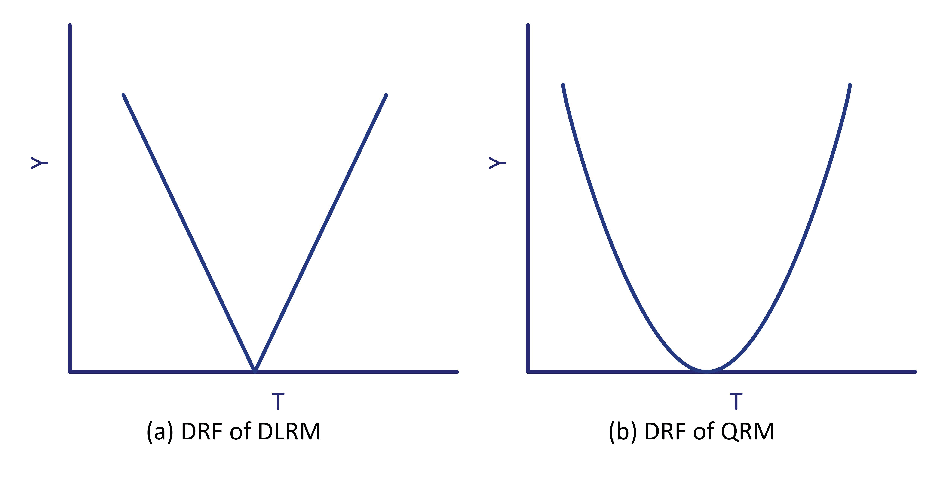
\includegraphics[width=0.7\textwidth]{DRF_curves.eps}
\caption{Matching units based on their propensity scores breaks the link between cofounding variables and treatment.}
%\vspace{-.5cm}
\label{DRF_curves}
\end{figure*}
\vspace{-0.1cm}

Finally, we chose to use the absolute value of fitted a regression coefficient's $t$-statistic [19] as a suspiciousness score, rather than the coefficient itself, because we wish to ``penalize" coefficients with large standard errors.  We use $\left| t \right|$ to denote the absolute value of the $t$-statistic for a fitted coefficient $\hat \beta $: $\left| t \right| = |\hat \beta /std ( {\hat \beta })|$ , where $std(\hat \beta)$ is the standard error of $\hat \beta$.  Thus, for DLRM the failure-causing effect of treatment $T_e$ is estimated by the summation of two linear regression models'$\left| t \right|$ values for the fitted slope coefficient ${{\hat \gamma }_e}$.  For QRM, this effect is estimated by the $\left| t \right|$ value of the estimated coefficient ${\hat \zeta }$ of the quadratic term of the regression model.

\renewcommand{\algorithmicrequire}{\textbf{Input:}}
\renewcommand{\algorithmicensure}{\textbf{Output:}}
\begin{algorithm}
  \captionof{figure}{ {\it NUMFL} Algorithm}\label{NUMFLalg}

  \begin{algorithmic}[1]
    \Require Subexpression value table $E=[T_e, \pmb{X}_e]$, with all values standardized, and type of model $M$
    \Ensure Suspiciousness scores $\tau \left( e \right)$ of subexpressions, sorted in descending order
    \For  {each subexpression $e$ }
        \State        $T_e \gets$ treatment variable of {\it i}th subexpression
        \State        $\pmb{X}_e\gets$ confounding variables of {\it i}th subexpression
        \If{ using GPS}
            \State Fit linear regression model ${T_e} = {\pmb{X}_e}'{\pmb{\beta} _e}$
        \ElsIf{using CBPS}
            \State Fit models for $Pr(T_e=k \mid \pmb{X}_e)$,
            \State$k = 1 \ldots K$, using multinomial logistic regression
        \EndIf
        \For  {each  ${\pmb{x}_{e,j}}$ }
            \State Estimate the propensity score for ${\pmb{x}_{e,j}}$ using fitted GPS or
            \State CBPS model(s).
        \EndFor
        \State Group the observations into $m$ roughly equal-size subclasses.
        \For  {each subclass $k$ }
            \If{ $M$ is DLRM }
                 \State Fit two linear regression models:
                 \State  $Y = {\gamma _{e,1}}{T_e} + b$   for observations $T_e>median(T_e)$
                 \State  $Y = {\gamma _{e,2}}{T_e} + b$   for observations $T_e \le median(T_e)$
                 \State  ${\tau _1} = t$-value of ${\gamma _{e,1}}$
                 \State  ${\tau _2} = t$-value of ${\gamma _{e,2}}$
                 \State ${\tau ^k} = |{\tau _1}| + |{\tau _2}|$
            \EndIf
            \If{$M$ is QRM}
                \State Fit quadratic regression model $Y = \zeta {T_e}^2 + \eta {T_e} + c$
                \State ${\tau ^k} = |t$-value of $\hat \zeta |$
            \EndIf
        \EndFor
        \State $\tau(e)$ = weighted average of  $\tau^k$ across $m$ subclasses
    \EndFor
    \State Sort  $\tau(e)$ values in descending order.

  \end{algorithmic}
\end{algorithm}


Figure \ref{NUMFLalg} shows the NUMFL-GPS algorithm.  Note that all input values are standardized $(x \to \frac{{x - \mu }}{\sigma })$ to adjust for differences in scale between variables.  NUMFL-GPS processes each numeric expression or subexpression e in three stages.  In the first stage (lines 2-5 and 10-14), it fits a linear propensity score model regressing the treatment variable $T_e$ on the confounding variables $X_e$, then uses the fitted model to calculate the generalized propensity score for each observation.  The scores are grouped into $m$ roughly equal-sized subclasses.  In the second stage (lines 15-28), the algorithm estimates the ``penalized" AFCE of $T_e$ on $Y$ separately in each subclass.  If DLRM is employed, the data within a subclass is split into two equal-size groups.  The algorithm fits a linear model for each group, and it records the {\it t}-statistics ${\tau _1}$ and ${\tau _2}$ for the coefficients of $T_e$ in the two models.  The penalized AFCE for subclass $k$ is given by the sum ${\tau ^k} = |{\tau _1}| + \left| {{\tau _2}} \right|$.  If QRM is employed, the algorithm fits a quadratic model and records the coefficient ${\hat \zeta }$ of the quadratic term.  The penalized AFCE for subclass $k$ is estimated by the absolute value of the {\it t}-statistic for ${\hat \zeta }$.  In the third stage, the overall AFCE or suspiciousness score $\tau(e)$ for subexpression $e$ is computed as a weighted average of $\tau^k$ over all subclasses $k$ (line 29).  Finally, the suspiciousness scores for all subexpressions are sorted in descending order (line 31).  The developer uses the sorted list to guide fault localization.

\subsection{NUMFL-CBPS}\label{IVB}
NUMFL-CPBS differs from NUMFL-GPS in that the former employs the Covariate Balancing Propensity Score instead of GPS for confounding control.   Recall from Section \ref{IIID} that the CBPS seeks to optimize covariate balance by employing the Generalized Method of Moments (GMM), which solves balance equations for the parameters of interest.

\subsubsection{Control of Confounding.}
In Imai and Ratkovic's extension of CBPS to treatment variables with $K>2$ discrete values \cite{Hansen1982}, a multinominal logistic regression model is used to estimate the conditional probability $\pi_{\pmb \beta}^k (\pmb{x})=Pr(T=k \mid \pmb{X})$ of treatment $k$. To handle a continuous treatment variable $T_e$ associated with a numerical expression $e$, we discretize the values of $T_e$ by partitioning them into ordered bins.  For each $k$, $1 \leq k<K$, the probability  that the original value of $T_e$ belongs in bin $k$ is modeled by
\begin{equation*}
\Pr ({T_e} = k \mid{\pmb{X}_e}) = \frac{{{e^{{{\pmb \beta} _k}{\pmb{x}_e}}}}}{{1 + \sum\nolimits_{i = 1}^{K - 1} {{e^{{{\pmb \beta} _i}{\pmb{x}_e}}}} }}
\end{equation*}
and
\begin{equation*}
\Pr ({T_e} = K\mid{\pmb{X}_e}) = \frac{1}{{1 + \sum\nolimits_{i = 1}^{K - 1} {{e^{{{\pmb \beta} _i}{\pmb{x}_e}}}} }}
\end{equation*}
The CBPS can be estimated using the open source R package ``CBPS" created by Fong, {\it et al} \cite{CBPS}.

The whole process of applying CBPS in NUMFL involves the following three steps:
\begin{enumerate}
\item 	Given a sample of observed values for the discretized treatment variable $T_e$ and for the covariates $\pmb{X}_e$, use the R package ``CBPS" to estimate the coefficients of a multinominal logistic propensity score model $\pi _{\pmb{\beta}} ^k({\pmb{x}_{e,i}}) = P({T_{e,i}} = k \mid {\pmb{x}_{e,i}})$ for each $k$.
\item	For each observed value ${\pmb x}_{e,i}$, estimate propensity score $\hat \pi _{e,i}$ with the fitted propensity score model.
\item Group observations with the same or similar values of $\hat \pi _{e,i}$ into $m$ subclasses of roughly equal size.
\end{enumerate}

Here $\hat \pi _{e,i}$ represents the calculated propensity score for each observed value.  Similar $\hat \pi _{e,i}$ values correspond to a set of $\pmb{x}_{e,i}$ values that influence the treatment similarly, so we group the observations into subclasses as we did in NUMFL-GPS.  Propensity score estimation and grouping in NUMFL-CBPS corresponds to lines 6-14 in the algorithm of Figure \ref{NUMFLalg}.

\subsubsection{Failure-causing Effect Estimation.}
Failure-causing-effect estimation in NUMFL-CBPS follows the same process followed in NUMFL-GPS, which is shown in lines 15-29 of Figure \ref{NUMFLalg}.  For a given subexpression $e$, QRM or DLRM is used to estimate the ``penalized" AFCE of $T_e$ on $Y$ within each subclass individually. Then the failure-causing effect is calculated as a weighted average the penalized AFCEs over all subclasses. Finally, the results for all subexpressions are sorted.

\begin{table*}[htbp!]
\caption{STANDARDIZED VARIABLE VALUES OF THE MOTIVATING EXAMPLE}
\label{exampledata2}
\centering
      \begin{tabular}{|l|c|c|c|c|c|c|c|c|c|c|}
      \hline
Test \#	&	1	&	2	&	3	&	4	&	5	&	6	&	7	&	8	&	9	&	10	\\	\hline
$a$	&	-0.166	&	0.876	&	0.183	&	0.091	&	-0.490	&	-0.235	&	-0.232	&	-0.382	&	0.831	&	-0.475	\\	\hline
$b$	&	-0.364	&	0.023	&	0.797	&	-0.433	&	-0.720	&	0.138	&	-0.381	&	0.746	&	0.233	&	-0.039	\\	\hline
$c$	&	-0.523	&	0.834	&	-0.218	&	0.113	&	-0.119	&	0.111	&	0.832	&	-0.646	&	-0.269	&	-0.114	\\	\hline
$k$	&	-0.336	&	0.580	&	0.619	&	-0.213	&	-0.769	&	-0.065	&	-0.389	&	0.222	&	0.683	&	-0.331	\\	\hline
$x$	&	-0.110	&	0.404	&	-0.079	&	-0.001	&	0.631	&	-0.204	&	0.431	&	-1.156	&	0.269	&	-0.186	\\	\hline
$r$	&	-0.027	&	0.517	&	0.358	&	-0.031	&	-0.460	&	0.478	&	-0.328	&	-1.027	&	0.501	&	0.020	\\	\hline
$Y$	&	2.552	&	1.592	&	0.882	&	0.335	&	0.490	&	0.896	&	2.102	&	5.611	&	0.900	&	1.065	\\	\hline
\end{tabular}
\end{table*}

We will use the expression $s_3$ and $s_8$ in the faulty code of motivating example shown in Figure\ref{code} to  demonstrate the NUMFL algorithm in Figure\ref{NUMFLalg} step by step. The variable values are come from  Table\ref{exampledata}. In the motivating example, we know that the bug exists in expression $s_3$, so the estimated suspiciousness score of $s_3$ should be larger than the estimated suspiciousness score of $s_8$. In practice, running the NUMFL algorithm requires decomposing complex numerical expression in to several subexpressons , which has relatively simple structure. But the expressions $s_3$ and $s_8$ already have simple structure, so we choose to estimate the AFCE of the expressions without decomposing them into subexpressions. 

For expression $s3$ , the first step is to identify the treatment variable and confounding variables. In the expression $s3$, the treatment variable $T_e$ is variable $x$ and the confounding variables are $a$, $b$ and $c$. Then we adjust  the differences in scale between variables by standardizing the variables' values. Table\ref{exampledata2} shows all the variables values after standardization. Note that the outcome variable $Y$ is not standardized. Next we estimate propensity scores for each observations. To estimate GPS ${\hat{\theta}}_{s_3}$, we can fit a linear regression model as described in section\ref{IIIC}. If NUMFL-CBPS is used, we need to fit a multinomial logistic regression model, which is some what complex. Here we use R package "CBPS" to estimate the CBPS which can automatically fit a multinomial regression model with the treatment variables and confounding variables and then estimate the propensity score. For the detail of the package "CBPS", the reader should refer to \cite{CBPS}. Table\ref{exampledata3} shows expression $s_3$'s  estimated GPS ${\hat{\theta}}_{s_3}$ and CBPS ${\hat{\pi}}_{s_3}$ for each observation. With the estimated propensity scores, we group observations with same or similar propensity scores into $m$ subclasses. For simplicity, we use $m=2$ for the motivating example. We rank the tests according to their propensity scores in descending order. The first 5 tests are in subclass 1 and the last 5 tests are in subclass 2. The last two columns of Table\ref{exampledata3} shows the subclass index of each test for NUMFL-GPS and NUMFL-CBPS. From Table\ref{exampledata3}, we can see there is some difference between the subclassification results of NUMFL-GPS and NUMFL-CBPS. In NUMFL-GPS, test 4 and test5 are in subclass 2 , while in NUMFL-CBPS, test4 and test5 belong to subclass1.  Similarly, we calculate GPS and CBPS for expression $s_8$, which is summarized in Table\ref{exampledata4}.  

The suspiciousness score of expression is estimated by the average of failure-causing effect in two subclasses. Assume we use QRM to estimate failure-causing effect,  a quadratic regression model $Y = \zeta {T_e}^2 + \eta {T_e} + c$  is fitted in each subclass. The $|t$-value$|$ of  the coefficient $\zeta$ is the estimated failure-causing effect. Table\ref{exampledata5} shows the estimated failure-causing effect in each subclass when NUMFL-GPS is used.  In Table\ref{exampledata5},  ${|t-value|}_1$ denotes the estimated failure-causing effect in subclass1 and ${|t-value|}_2$ denotes the estimated failure-causing effect in subclass2. The estimated suspiciousness score (AFCE) is equal to  $({{|t-value|}_1}+{{|t-value|}_2})/2$. For comparison, we also fit a quadratic regression model with full sample without subclassification and the estimated failure-causing effect is denoted by ${|t-value|}_0$. In Table\ref{exampledata5}, ${|t-value|}_0$ of $s_8$ is close to ${|t-value|}_0$ of $s_3$, even though $s_8$ is not faulty. This is because the faulty variable $x$ in $s_3$ is confounder of variable $r$ in  $s_8$ and make $s_8$ associate to program failure. When NUMFL-GPS is applied, the estimated AFCE of $s_8$ is significantly smaller than the estimated AFCE of $s_3$. The estimated suspiciousness scores of NUMFL-CBPS are shown in  Table\ref{exampledata6}. In Table\ref{exampledata6}, the difference between  $s_3$ and $s_8$'s suspiciousness score is larger than the difference between their ${|t-value|}_0$s. This means both GPS and CBPS are effective in controlling confounding bias.  


\begin{table*}[htbp!]
\caption{ESTIMATED GPS AND CBPS OF EXPRESSION $s_3$}
\label{exampledata3}
\centering
      \begin{tabular}{|l|c|c|c|c|}
      \hline
Test \#	&	${\hat{\theta}}_{s_3}$	&	${\hat{\pi}}_{s_3}$	&	Subclass index (GPS)	&	Subclass index (CBPS)	\\ \hline
1	&	0.057	&	0.847	&	2	&	2	\\ \hline
2	&	0.364	&	0.716	&	2	&	2	\\ \hline
3	&	-0.606	&	5.65E-11	&	1	&	1	\\ \hline
4	&	0.310	&	5.05E-06	&	2	&	1	\\ \hline
5	&	0.692	&	1.60E-09	&	2	&	1	\\ \hline
6	&	-0.143	&	5.872	&	1	&	2	\\ \hline
7	&	0.637	&	2.570	&	2	&	2	\\ \hline
8	&	-1.119	&	5.22E-06	&	1	&	1	\\ \hline
9	&	-0.113	&	0.130	&	1	&	1	\\ \hline
10	&	-0.079	&	5.694	&	1	&	2	\\ \hline
\end{tabular}
\end{table*}

\begin{table*}[htbp!]
\caption{ESTIMATED GPS AND CBPS OF EXPRESSION $s_8$}
\label{exampledata4}
\centering
      \begin{tabular}{|l|c|c|c|c|}
      \hline
Test \#	&	${\hat{\theta}}_{s_8}$	&	${\hat{\pi}}_{s_8}$	&	Subclass index (GPS)	&	Subclass index (CBPS)	\\ \hline
1	&	-0.258	&	0.521	&	1	&	2	\\ \hline
2	&	0.562	&	3.156	&	2	&	2	\\ \hline
3	&	0.323	&	3.878	&	2	&	2	\\ \hline
4	&	-0.127	&	3.099	&	1	&	2	\\ \hline
5	&	-0.110	&	0.004	&	2	&	1	\\ \hline
6	&	-0.149	&	1.14E-07	&	1	&	1	\\ \hline
7	&	0.005	&	0.008	&	2	&	1	\\ \hline
8	&	-0.498	&	1.51E-06	&	1	&	1	\\ \hline
9	&	0.549	&	3.079	&	2	&	2	\\ \hline
10	&	-0.297	&	0.069	&	1	&	1	\\ \hline
\end{tabular}
\end{table*}

\begin{table*}[htbp!]
\caption{ESTIMATED AFCE WITH NUMFL-GPS}
\label{exampledata5}
\centering
      \begin{tabular}{|l|c|c|c|c|}
      \hline
Expression& ${|t-value|}_1$  & ${|t-value|}_2$ & Suspiciousness score & ${|t-value|}_0$\\	\hline

$s_3$ &  13.861 &0.228 &7.045 &2.763 \\	\hline
$s_8$& 1.045 &0.515 &0.78 &2.601\\	\hline
\end{tabular}
\end{table*}

\begin{table*}[htbp!]
\caption{ESTIMATED AFCE WITH NUMFL-CBPS}
\label{exampledata6}
\centering
      \begin{tabular}{|l|c|c|c|c|}
      \hline
Expression& ${|t-value|}_1$  & ${|t-value|}_2$  & Suspiciousness score & ${|t-value|}_0$\\	\hline
$s_3$ &  4.034 &2.219 &3.127 &2.763\\	\hline
$s_8$& 1.898&0.325 &1.112 &2.601\\	\hline
\end{tabular}
\end{table*}

\section{EMPIRICAL EVALUATION}\label{evaluation}
To evaluate the effectiveness of NUMFL, we conducted an empirical study involving several subject programs, in which the performance of NUMFL was compared with the performance of several baselines techniques. In the study, we investigated four main research questions:  (1) What is the performance of NUMFL compare to baseline techniques when each subject program version contains only one fault?  (2) What is the performance of NUMFL compare to the baselines when each subject program version contains two faults?   (3) Given data from only failing executions, is NUMFL effective?  (4) Which is most effective, NUMFL-GPS or NUMFL-CBPS?

\subsection{Experimental Platform and Data Collection}
We developed a data collection and analysis platform for numerical fault localization studies involving Java programs.  The platform is based on a modified Java parser \cite{Java} and the ASM Java bytecode manipulation framework \cite{ASM}.  We first parse the source code of a subject program.  Each complete numerical expression is decomposed into a set of subexpressions as described in Section \ref{IVA}.  The ASM compiler is used to instrument the bytecode files of the subject program to record variable values used and produced by the evaluation of each subexpression.  Information is recorded to permit the recorded values to be mapped back to the corresponding source-code subexpressions.  Each instrumented subject program is executed on a test suite and the induced variable values are recorded.  For a subexpression within a loop, we currently record the associated values only for the last iteration of the loop, in order to reduce overhead.

The data collection algorithm is implemented in Java and can be downloaded from \cite{NUMFL}.  The NUMFL algorithm and other baseline techniques were implemented using the R statistical computing environment \cite{R}. In this study, the number of propensity score subclasses used in the NUMFL algorithm was set to 10.

\subsection{Subject Programs, Faults, and Tests}
{\bf Subject Programs.}  For the empirical study, we selected 16 subject programs from four Java numerical libraries: (1) Apache Common Math (versions 2.1 and 3.1.1), which is a popular Java library for scientific computing \cite{Commons}; (2) the Oj! Algorithms library Ojalgo (version 33.0), which is an open source Java library for mathematics, linear algebra and optimization \cite{Oj}; (3) JAMA, which is a basic linear algebra package for Java \cite{JAMA}; and (4) SciMark 2.0, which is a Java benchmark for measuring the performance of numerical codes occurring in scientific applications \cite{SciMark}.  We chose subject programs whose purpose we understood (so that we would be able to write tests for them if necessary) and having as many numerical expressions as possible.  We chose four large ($\ge 1500$ SLOC) and eight small subject programs ($< 1500$ SLOC) from Apache Common Math; for Ojalgo, we wrote a subject program to calculate the Schur decomposition of a matrix that uses two Ojalgo classes (PrimitiveDenseStore and HermitianEVD32); for JAMA, we created one subject program that uses four different matrix decomposition algorithms; we used two of SciMark's five computation kernels as subject programs, FFT and LU factorization.  A summary of our subject programs is shown in Table \ref{subpro}.

\begin{table*}[htbp!]
\caption{SUMMARY OF SUBJECT PROGRAMS}
\label{subpro}
      \begin{tabular}{|l|c|c|c|c|}
      \hline
Subject Program	&	SLOC	&	\# of Sub-expressions	&	\# of Tests	&	\# Faulty versions	\\	\hline
Apache\_EigenDecompose	&	1858	&	611	&	8000	&	10	\\	\hline
Apache\_DScompiler	&	1774	&	220	&	5000	&	10	\\	\hline
Apache\_BigMatrix	&	1580	&	244	&	3000	&	10	\\	\hline
Apache\_Rotation3D	&	1704	&	504	&	3000	&	10	\\	\hline
Ojaljo\_SchurDecompose	&	2129	&	649	&	5000	&	10	\\	\hline
Jama\_MatrixDecompose	&	1952	&	578	&	5000	&	10	\\	\hline
SciMark\_LU	&	295	&	35	&	3000	&	2	\\	\hline
SciMart\_FFT	&	197	&	59	&	3000	&	2	\\	\hline
Apache\_SymmLQ	&	1226	&	57	&	5000	&	2	\\	\hline
Apache\_SplineInterpolator	&	130	&	45	&	5000	&	2	\\	\hline
Apche\_SimpleRegress	&	869	&	61	&	5000	&	2	\\	\hline
Apache\_SchurTransformer	&	458	&	154	&	3000	&	2	\\	\hline
Apache\_MillerUpdatRegress	&	1110	&	152	&	1000	&	2	\\	\hline
Apache\_HarmonicFitter	&	385	&	50	&	3000	&	2	\\	\hline
Apache\_FastSine	&	197	&	66	&	5000	&	2	\\	\hline
Apache\_FastCosine	&	188	&	77	&	5000	&	2	\\	\hline
\end{tabular}
\end{table*}

{\bf Faults.}  To evaluate NUMFL, we required faulty versions of subject programs.  After much searching, we were able to find few well documented faults (including fixes) that produced numerical output that was sometimes, but not always, incorrect.  Hence, we {\it injected} three types of simulated numerical faults into the subject programs: (1) adding a small random number to a numerical expression (the number varied between and within runs); (2) multiplying a numerical expression by a random number; (3) randomly changing one of the operators of a numerical expression (once only).  Each faulty version of a subject program contained one bug.  We generated 12 faulty versions of each subject program whose number of lines of source code was larger than 1500.  For each subject program with fewer than 1500 SLOC, we generated two faulty versions.  Except for SciMark, every subject program came with a unit test suite which provided a predefined error tolerance; we chose a tolerance of 1.0E-5 for SciMark.  We ran the faulty versions of the subject programs and the original correct versions with the same inputs.  If the output error $Y$ exceeded the tolerance, the execution was considered to be failure.  If the subject program's output was a scalar variable, the output error $Y$ was the absolute difference between the correct and faulty programs' outputs.  If the subject program's output was an array, we calculated the difference between each element in the faulty program's output and the corresponding element in correct program's output.  The output error $Y$ was taken to be the first difference encountered that was larger than the tolerance or zero if no such difference was found.


{\bf Tests.}  Since a number of our subject programs came with very few test cases, it was necessary to create test cases for them.  We first analyzed the subject programs and the test cases provided by their developers. Then we randomly generated inputs similar to those of the test cases. Note that for NUMFL, we did not generally use the total number of tests shown in Table \ref{subpro}, though we did so for the baseline techniques.  Instead, we first selected all $N$ tests of the smaller of the set of failed tests and the set of passed tests, and we then randomly selected $N$ tests from the larger set. (See Section \ref{VE} for an exception.)

\subsection{Baseline SFL Metrics and Cost Measure}

{\bf Baselines.}  We compared NUMFL to four baseline SFL metrics.  Two are coverage-based metrics that have performed well in comparisons with other such metrics: Ochiai \cite{Abreu2007} and DStar (with $star = 2$) \cite{Wong2014}.   The Ochiai metric estimates the suspiciousness of a statements $s$ with the equation
\begin{equation}
O(s) = {f_s}/\sqrt {f({f_s} + {p_s})}
\end{equation}
where: $f_s$ is the number of failed tests that cover statement $s$; $p_s$ is number of passed tests that cover $s$; and $f$ is the total number of failed tests.  The Dstar metric (with $star = 2$) is
\begin{equation}
D(s) = {f_s}^2/({p_s} + f - {f_s})
\end{equation}
where $f-f_s$ is the number of failed tests that do not cover $s$.

The other two baselines are predicate-level SFL metrics, SOBER \cite{Liu2005} and the Exploratory Software Predictor (ESP) \cite{Gore2011}.  SOBER computes the probability $\pi(P)$ that a predicate $P$ evaluated to be true in an execution.  If the distribution of $\pi(P)$ in passing runs differs significantly from its distribution in failing runs then $P$ is considered to be related to the fault.  In this study, for a treatment variable $T_e$ we use these predicates [20]: $T_e>0$, $T_e=0$ and $T_e<0$.

ESP employs ``elastic predicates" to partition the value space for each variable $x$ at each assignment to $x$.  ESP provides two instrumentation schemes: single variable and scalar pairs.  The single variable scheme uses execution profiles to compute the mean $\mu_x$ and standard deviation $\sigma_x$ for a variable $x$.  These statistics are then used in nine predicates (e.g., $x<\mu_x+\sigma_x$) that collectively partition the values of $x$ for three standard deviations above and below $\mu_x$.  ESP then computes an importance score for each predicate.  The suspiciousness of each assignment to $x$ is taken to be the highest importance score among the corresponding elastic predicates.  In a similar way, the scalar pair [31] scheme addresses differences in the values of pairs of variables (e.g.,  $x-y>\mu_{x-y}+\sigma_{x-y}$).

{\bf Cost Measure.}  We measured the costs of applying NUMFL and the baseline metrics by the percentage of {\it subexpressions} that need to be examined, in decreasing order of suspiciousness scores, to find the fault, assuming the fault is recognized when it is encountered.  This contrasts with most SFL techniques, which localize faults at the statement level.  There are two reasons that we chose to have NUMFL compute suspiciousness scores for subexpressions rather than for statements.  First, the location of a faulty subexpression not only implies the location of the numerical statement that contains the subexpression, but it also indicates which part of the statement is problematic.   Second, in this study we collected data only for floating point variables involved in numerical expressions.   As a result, the number of subexpressions was usually smaller than the number of lines of code.  To ensure a fair comparison between NUMFL and the predicate-level baseline metrics, predicates were associated with subexpressions.  In comparing NUMFL to the statement-level, coverage-based baseline metrics, subexpressions belonging to same statement received the {\it same suspiciousness score}.   To compare NUMFL fairly to the latter metrics, if multiple subexpressions got the same suspiciousness score as the faulty subexpression, we considered the faulty subexpression to rank in the middle of them.

\subsection{Comparative Performance of NUMFL vs. Baselines}\label{VD}
Table \ref{table2} shows, for NUMFL-GPS and the baseline metrics and for each subject program, the average percentage of subexpressions that had to be examined to find the fault, computed across all the faulty versions.  Here we show the results for QRM but not for DLRM, which QRM outperformed.  (Nevertheless, DLRM outperformed the 5 baseline metrics.)  For 14 of 16 subject programs, NUMFL-GPS-QRM performed better than Ochiai, DStar ($star=2$), and SOBER. NUMFL-GPS-QRM performed better than ESP-SIV (single variable) and ESP-SCP (scalar pair) for all 16 subject programs.  Overall, NUMFL-GPS-QRM was more effective in localizing numerical faults than any of the baseline metrics.
\begin{table*}[htbp!]
\fontsize{8pt}{9pt}\selectfont
\centering
\caption{AVERAGE FAULT LOCALIZATION COSTS OF NUMFL-GPS-QRM AND BASELINE METRICS ON SINGLE-FAULT PROGRAM VERSIONS}
\label{table2}
      \begin{tabular}{|l|c|c|c|c|c|c|}
      \hline
\multirow{2}{*}{{\bf Subject Program}}	&	\multicolumn{6}{|c|}{{\bf Technique}}	\\	\cline{2-7}
&{NUMFL-GPS-QRM}	&{ Ochiai}&	{ Dstar}&	{ ESP(SIV)} &	{ ESP(SCP)}	&{SOBER} \\\hline
Apache\_EigenDecompose	&	12.3\%	&	9.2\%	&	9\%	&	22.2\%	&	17.2\%	&	7.8\%	\\	\hline
Apache\_DScompiler	&	11\%	&	19.9\%	&	16.5\%	&	22.9\%	&	18.9\%	&	24.2\%	\\	\hline
Apache\_BigMatrix	&	11.4\%	&	51.8\%	&	51.8\%	&	37.9\%	&	31.8\%	&	28.9\%	\\	\hline
Apache\_Rotation3D	&	8\%	&	30.5\%	&	30.5\%	&	20.1\%	&	23.6\%	&	28.5\%	\\	\hline
Ojaljo\_SchurDecompose	&	11.4\%	&	22.7\%	&	22.7\%	&	20.2\%	&	27.3\%	&	30.9\%	\\	\hline
Jama\_MatrixDecompose	&	14.2\%	&	11.4\%	&	11.4\%	&	24.3\%	&	27\%	&	46.4\%	\\	\hline
SciMark\_LU	&	15.3\%	&	38.9\%	&	68.1\%	&	27.8\%	&	18.8\%	&	12.5\%	\\	\hline
SciMart\_FFT	&	9.5\%	&	48.3\%	&	75\%	&	68.1\%	&	36.6\%	&	12.5\%	\\	\hline
Apache\_SymmLQ	&	2.6\%	&	37.7\%	&	85.1\%	&	7\%	&	10.5\%	&	32.9\%	\\	\hline
Apache\_SplineInterpolator	&	31.7\%	&	51.1\%	&	47.8\%	&	65\%	&	64.4\%	&	56.1\%	\\	\hline
Apche\_SimpleRegress	&	4.3\%	&	49.2\%	&	29.9\%	&	7.3\%	&	7.2\%	&	7.9\%	\\	\hline
Apache\_SchurTransformer	&	3.3\%	&	8.2\%	&	8.2\%	&	36.2\%	&	10.2\%	&	44.4\%	\\	\hline
Apache\_MillerUpdatRegress	&	7.5\%	&	12.7\%	&	12.7\%	&	37.6\%	&	19.6\%	&	14.5\%	\\	\hline
Apache\_HarmonicFitter	&	27.3\%	&	45\%	&	58.5\%	&	39.5\%	&	41.7\%	&	49.3\%	\\	\hline
Apache\_FastSine	&	1.5\%	&	30.2\%	&	87.1\%	&	41.9\%	&	3.8\%	&	26.7\%	\\	\hline
Apache\_FastCosine	&	1.3\%	&	33.2\%	&	94.9\%	&	79.7\%	&	41.4\%	&	31.2\%	\\	\hline
Average Cost	&	10.8\%	&	31.3\%	&	44.3\%	&	34.9\%	&	25\%	&	28.4\%	\\	\hline
\end{tabular}
\end{table*}


We also compare the performance of NUMFL-GPS-QRM to that of each baseline SFL metric graphically. The comparison measure is the difference between the cost for the baseline metric and the cost for NUMFL-GPS-QRM.  Since the two costs are percentages, the difference is the percentage reduction in cost obtained by using NUMFL-GPS-QRM, which may be positive or negative.  For example, if the cost of using NUMFL-GPS-QRM is 10\% and the cost of using the baseline metric is 40\%, then the improvement is 30\%.  Figure \ref{QRM_VS_Base} shows the results of comparisons of NUMFL-GPS-QRM with each of the baseline metrics.  In each graph, the vertical axis represents the percentage improvement (reduction) in cost. The horizontal-axis represents different subject-program versions for which there are cost differences between the metrics, with each version represented by a vertical bar.   Bars above the zero-line represent versions for which NUMFL-GPS-QRM performed better than the baseline metric and bars below zero represent versions for which NUMFL-GPS-QRM performed worse.  The length of each bar represents the magnitude of the corresponding cost difference.

\textit{\textbf{ NUMFL-GPS-QRM vs. Ochiai.}}  Over all 92 faulty subject-program versions, NUMFL-GPS-QRM performed better than the Ochiai metric on 67 versions but NUMFL-GPS-QRM performed worse on 25 versions.  There were 38 versions for which NUMFL-GPS-QRM performed at least 20\% better than the Ochiai metric.  There were just 5 versions for which the latter performed better than NUMFL-GPS-QRM.

\textit{\textbf{ NUMFL-GPS-QRM vs. DStar.}}  NUMFL-GPS-QRM performed better than DStar on 70 subject-program versions but NUMFL-GPS-QRM performed worse than DStar on 22 versions.  NUMFL-GPS-QRM performed at least 20\% better than DStar on 42 versions, whereas DStar performed at least 20\% better than NUMFL-GPS-QRM on just 5 versions.

\textit{\textbf{ NUMFL-GPS-QRM vs. ESP-SIV.}} NUMFL-GPS-QRM performed better than ESP-SIV on 70 subject-program versions but NUMFL-GPS-QRM performed worse than ESP-SIV on 22 versions.  NUMFL-GPS-QRM performed at least 20\% better than ESP-SIV on 31 versions, whereas ESP-SIV performed at least 20\% better than NUMFL-GPS-QRM on just 5 versions.

\textit{\textbf{ QRM vs. ESP-SCP.}}  NUMFL-GPS-QRM performed better than ESP-SCP on 61 subject-program versions but NUMFL-GPS-QRM performed worse than ESP-SCP on 31 versions.  NUMFL-GPS-QRM performed at least 20\% better than ESP-SIV on 27 versions, whereas ESP-SCP performed at least 20\% better than NUMFL-GPS-QRM on just 3 versions.

\textit{\textbf{ QRM vs. SOBER.}}  NUMFL-GPS-QRM performed better than SOBER on 64 subject-program versions but NUMFL-GPS-QRM performed worse than SOBER on 28 versions.  NUMFL-GPS-QRM performed at least 20\% better than SOBER on 32 versions, whereas SOBER performed at least 20\% better than NUMFL-GPS-QRM on just 7 versions.

% figure example
%\begin{landscape}
\begin{sidewaysfigure}
\centering
\includegraphics[width=\textwidth]{QRM_VS_Base.eps}
\caption{Performance of NUMFL-GPS-QRM relative to baseline metrics on individual single-fault program versions.}
\label{QRM_VS_Base}
\end{sidewaysfigure}
%\end{landscape}

\subsection{NUMFL-GPS Applied only to Failing Runs}\label{VE}
Conventional, coverage-based and predicate-based SFL techniques require profiles and PASS/FAIL labels from both passing and failing runs, in order to rank statements based on estimates of quantities like $Pr [failure \mid s covered]$ \cite{Baah2010} that vary between statements only if the data come from a mix of passing and failing runs.  However, because many numerical programs have few conditional branches, a particular fault may be executed and cause erroneous values to occur on every run that is observed.  If these values propagate to the program output, a failure may occur on every run, depending on the numerical accuracy required.


Even if it is applied to data from only failing runs, NUMFL can still produce different AFCE estimates for different statements, because the causal outcome of interest is a continuous variable--the output error of a numerical program.  To evaluate whether NUMFL-GPS is actually effective when it is applied to data from only failing runs, we redid the study just described, after creating a new data set by removing the data from passing runs.  Table \ref{table3} and Figure \ref{QRM_allFail} compare the performance of QRM with such data to its performance with the original data from both passing and failing runs.  Figure \ref{QRM_allFail} shows that over all 92 faulty subject-programs versions, QRM performed better with data from only failing runs on 43 program versions and it performed worse on 49 versions.  There were only 8 versions for which QRM performed at least 20\% worse with data from only failing runs.

\begin{table*}[htbp!]
\caption{AVERAGE FAULT LOCALIZATION COSTS OF NUMFL-GPS-QRM WITH AND WITHOUT DATA FROM PASSING RUNS, ON SINGLE-FAULT PROGRAM VERSIONS}
\label{table3}
\centering
      \begin{tabular}{|l|c|c|}
      \hline
\multirow{2}{*}{{\bf Subject Program}}	&	\multicolumn{2}{|c|}{{\bf Input}}	\\	\cline{2-3}
& Pass and Fail	&Fail only \\ \hline
Apache\_EigenDecompose	&	12.3\%	&	11.4\%	\\	\hline
Apache\_DScompiler	&	11\%	&	11\%	\\	\hline
Apache\_BigMatrix	&	11.4\%	&	8\%	\\	\hline
Apache\_Rotation3D	&	8\%	&	18.9\%	\\	\hline
Ojaljo\_SchurDecompose	&	11.4\%	&	17.7\%	\\	\hline
Jama\_MatrixDecompose	&	14.2\%	&	24.5\%	\\	\hline
SciMark\_LU	&	15.3\%	&	54.1\%	\\	\hline
SciMart\_FFT	&	9.5\%	&	17.2\%	\\	\hline
Apache\_SymmLQ	&	2.6\%	&	2.6\%	\\	\hline
Apache\_SplineInterpolator	&	31.7\%	&	21.7\%	\\	\hline
Apche\_SimpleRegress	&	4.3\%	&	3.4\%	\\	\hline
Apache\_SchurTransformer	&	3.3\%	&	8.2\%	\\	\hline
Apache\_MillerUpdatRegress	&	7.5\%	&	12.7\%	\\	\hline
Apache\_HarmonicFitter	&	27.3\%	&	47.5\%	\\	\hline
Apache\_FastSine	&	1.5\%	&	1.5\%	\\	\hline
Apache\_FastCosine	&	1.3\%	&	1.3\%	\\	\hline
Average Cost	&	10.8\%	&	16.4\%	\\	\hline
\end{tabular}
\end{table*}

% figure example
\begin{figure*}[!thpb]
\centering
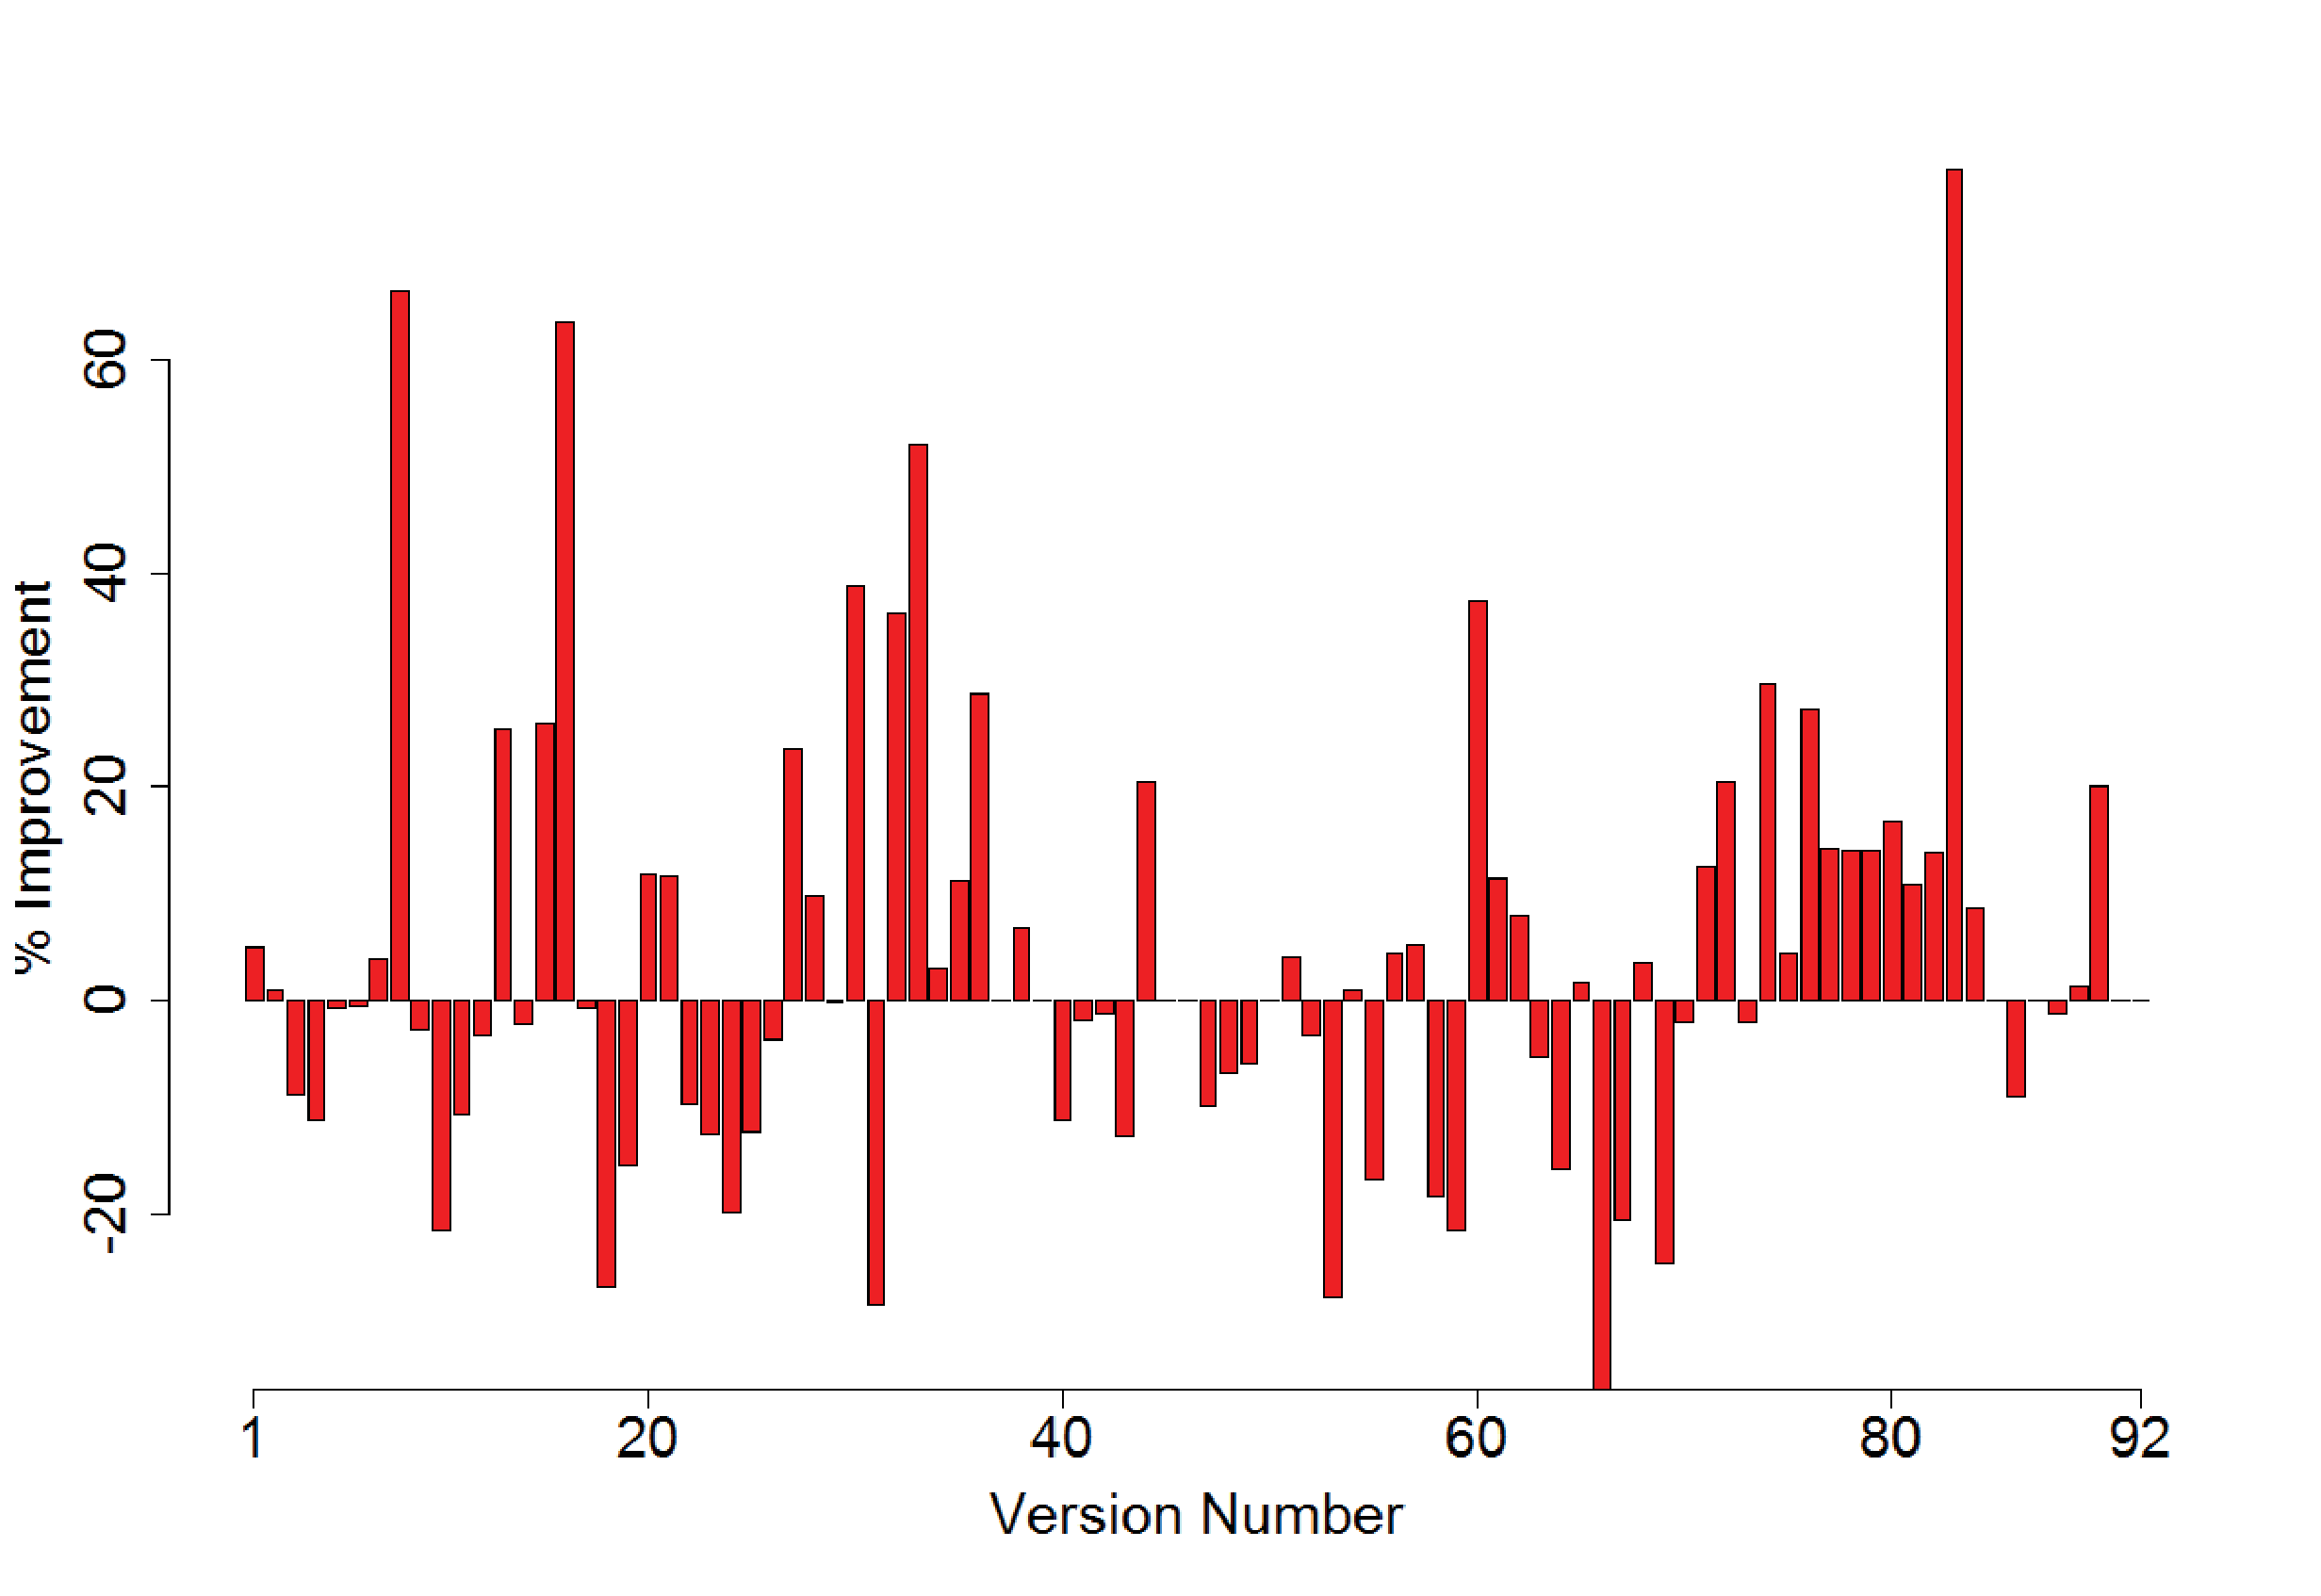
\includegraphics[width=0.6\textwidth]{QRM_allFail.eps}
\caption{Relative performance of NUMFL-GPS-QRM with and without data from passing runs, on individual single-fault program versions.}
\label{QRM_allFail}
\end{figure*}

From Table \ref{table3} and Figure \ref{QRM_allFail}, we can see that NUMFL works fairly well for most subject programs when used with data from only failing runs, although its performance is generally better with data from both passing and failing runs.  Note that with many numerical programs the tolerance for output errors is very small (between 1.0E-5 and 1.0E-12).  For such programs, the output errors from passing runs are clustered around 0, while output errors from failing runs are larger and more varied.  Consequently, the data from failing runs carries more information about the dose-response function than does the data from the passing runs.  Hence, using only data from failing runs to estimate the DRF does not necessarily result in severe bias.

\subsection{Application of NUMFL-GPS to Programs with Multiple Faults}
The empirical results presented in Section \ref{VD} indicate that NUMFL-GPS performs better than the baseline techniques on the subject program versions containing a single fault.  This section reports on the application of NUMFL-GPS to subject program versions with multiple faults.  For this sub-study, we selected five of the larger subject programs (shown in Table \ref{table4}) and generated 5 faulty versions of each for a total of 25 faulty versions.  To create each faulty version, we randomly injected two simulated faults. (Injecting a larger number of faults in our programs tended to make them fail badly on all inputs).  Table \ref{table4} shows the average cost, over the faulty versions of each subject program, of localizing the first fault to be found, for NUMFL-GPS-QRM and each of the baseline techniques.  The table shows that NUMFL-GPS-QRM outperformed the other baseline techniques on average, although SOBER and Ochiai each performed better on one of the subject programs.
\begin{table*}[htbp!]
\fontsize{8pt}{9pt}\selectfont
\centering
\caption{AVERAGE FAULT LOCALIZATION COSTS OF NUMFL-GPS-QRM AND BASELINE METRICS ON SINGLE-FAULT PROGRAM VERSIONS}
\label{table4}
      \begin{tabular}{|l|c|c|c|c|c|c|}
      \hline
\multirow{2}{*}{{\bf Subject Program}}	&	\multicolumn{6}{|c|}{{\bf Technique}}	\\	\cline{2-7}
&{NUMFL-GPS-QRM}	&Ochiai&	Dstar&	ESP(SIV) &	ESP(SCP)	&SOBER \\\hline
Apache\_EigenDecompose	&	10.3\%	&	20\%	&	19.4\%	&	28.3\%	&	25.8\%	&	6.3\%	\\	\hline
Apache\_DScompiler	&	4.5\%	&	31.5\%	&	23.2\%	&	19.9\%	&	10.4\%	&	9\%	\\	\hline
Apache\_Rotation3D	&	7\%	&	3.6\%	&	33.6\%	&	17.5\%	&	17.9\%	&	25.8\%	\\	\hline
Ojaljo\_SchurDecompose	&	5.4\%	&	22.7\%	&	27.1\%	&	8.4\%	&	9.6\%	&	27.1\%	\\	\hline
Jama\_MatrixDecompose	&	14.1\%	&	26.3\%	&	16.5\%	&	26.3\%	&	26.2\%	&	15.5\%	\\	\hline
Average Cost	&	8.3\%	&	20.8\%	&	24\%	&	20.1\%	&	18\%	&	16.7\%	\\	\hline
\end{tabular}
\end{table*}

Figure \ref{QRM_VS_Base_MultipleFault} graphically contrasts the performance of NUMFL-GPS-QRM on the individual two-fault program versions with that of the baseline metrics.  It is evident that SOBER's performance is the second best after NUMFL-GPS-QRM.  Over all 25 faulty subject-program versions, NUMFL-GPS-QRM performed better than SOBER on 15 versions but performed worse on 10 versions.  There were 8 versions for which NUMFL-GPS-QRM performed at least 10\% better than SOBER but only one version for which SOBER performed at least 10\% better than NUMFL-GPS-QRM.  Both Ochiai and ESP-SCP performed better than NUMFL-GPS-QRM on 8 versions but performed worse on 17 versions.  NUMFL-GPS-QRM performed better than ESP-SIV on 19 versions and performed better than DStar on 21 versions.
\begin{figure*}[!thpb]
\centering
\includegraphics[width=\textwidth]{QRM_VS_Base_MultipleFault.eps}
\caption{Performance of GPS-QRM relative to baseline metrics on individual two-fault program versions .}
\label{QRM_VS_Base_MultipleFault}
\end{figure*}

\subsection{Comparison of NUMFL-GPS and NUMFL-CBPS}
In this section, we report the results of empirically comparing the performance of NUMFL-GPS-QRM with that of NUMFL-CBPS-QRM.  We applied the two techniques to the subject program versions with single faults as well as to the versions with two faults.  The average fault localization costs on the single fault versions is shown in Table \ref{table5}.  There were 13 versions for which NUMFL-GPS-QRM performed better than NUMFL-CBPS-QRM. There were only 3 versions for which NUMFL-CBPS-QRM performed better than NUMFL-GPS-QRM. Figure \ref{CBPS_VS_GPS} graphically contrasts the performance of the two methods on the single fault versions.  NUMFL-GPS-QRM performed better on 61 versions, while NUMFL-CBPS-QRM performed better on 31 versions.  NUMFL-GPS-QRM performed at least 20\% better than NUMFL-CBPS-QRM on 15 versions, whereas NUMFL-CBPS-QRM performed at least 20\% better than NUMFL-GPS-QRM on just 4 versions.

\begin{table*}[htbp!]
\caption{AVERAGE FAULT LOCALIZATION COSTS OF NUMFL-GPS-QRM AND NUMFL-CBPS-QRM ON SINGLE-FAULT PROGRAM VERSIONS }
\label{table5}
\centering
      \begin{tabular}{|l|c|c|}
      \hline
\multirow{2}{*}{{\bf Subject Program}}	&	\multicolumn{2}{|c|}{{\bf NUMFL}}	\\	\cline{2-3}
&  GPS-QRM	&CBPS-QRM \\ \hline
Apache\_EigenDecompose	&	12.3\%	&	8.8\%	\\	\hline
Apache\_DScompiler	&	11\%	&	12\%	\\	\hline
Apache\_BigMatrix	&	11.4\%	&	9.9\%	\\	\hline
Apache\_Rotation3D	&	8\%	&	18.9\%	\\	\hline
Ojaljo\_SchurDecompose	&	11.4\%	&	14\%	\\	\hline
Jama\_MatrixDecompose	&	14.2\%	&	23\%	\\	\hline
SciMark\_LU	&	15.3\%	&	27.8\%	\\	\hline
SciMart\_FFT	&	9.5\%	&	19.8\%	\\	\hline
Apache\_SymmLQ	&	2.6\%	&	4.4\%	\\	\hline
Apache\_SplineInterpolator	&	31.7\%	&	35\%	\\	\hline
Apche\_SimpleRegress	&	4.3\%	&	17\%	\\	\hline
Apache\_SchurTransformer	&	3.3\%	&	14.9\%	\\	\hline
Apache\_MillerUpdatRegress	&	7.5\%	&	9.9\%	\\	\hline
Apache\_HarmonicFitter	&	27.3\%	&	32\%	\\	\hline
Apache\_FastSine	&	1.5\%	&	13\%	\\	\hline
Apache\_FastCosine	&	1.3\%	&	1.2\%	\\	\hline
Average Cost	&	10.8\%	&	16.4\%	\\	\hline
\end{tabular}
\end{table*}

Table \ref{table6} shows the average cost, over the faulty versions of each subject program into which two faults were injected, of localizing the first fault to be found, for both NUMFL-GPS-QRM and NUMFL-CBPS-QRM.  NUMFL-GPS-QRM performed better than NUMFL-CBPS-QRM on the two-fault versions of 4 subject programs. NUMFL-GPS-QRM performed worse than NUMFL-CBPS-QRM on the versions of 1 subject program.  Figure \ref{CBPS_VS_GPS_MultipleFault} graphically contrasts the performance of the two methods on the individual two-fault versions.  NUMFL-GPS-QRM performed better than NUMFL-CBPS-QRM on 13 versions and NUMFL-GPS-QRM performed worse on 12 versions.  NUMFL-GPS-QRM performed at least 10\% better than NUMFL-CBPS-QRM on 7 versions, whereas NUMFL-CBPS-QRM performed at least 10\% better than NUMFL-GPS-QRM on just 1 version.

In summary, NUMFL-GPS-QRM performed better than NUMFL-CBPS-QRM on both single-fault and two-fault programs.  The generalized propensity score model $\pmb{\theta}=\pmb{X}'\pmb{\beta}$ achieved better covariate balance than the multinomial logistic regression model used with CBPS.  This may be due to the composition of the data collected from our subject program versions.  The performance of NUMFL-CBPS was poorest with versions that had no more than about 150 failing executions.  However, although NUMFL-CBPS performed worse than NUMFL-GPS in our study, the former's average fault localization cost was still lower than those of the baseline techniques.
\begin{table*}[htbp!]
\caption{AVERAGE FAULT LOCALIZATION COSTS OF NUMFL-GPS-QRM AND NUMFL-CBPS-QRM ON MULTIPLE-FAULT PROGRAM VERSIONS}
\label{table6}
\centering
      \begin{tabular}{|l|c|c|}
      \hline
\multirow{2}{*}{{\bf Subject Program}}	&	\multicolumn{2}{|c|}{{\bf NUMFL}}	\\	\cline{2-3}
&  GPS-QRM	&CBPS-QRM \\ \hline
Apache\_EigenDecompose	&	10.3\%	&	11.1\%	\\	\hline
Apache\_DScompiler	&	4.5\%	&	5.9\%	\\	\hline
Apache\_Rotation3D	&	7.0\%	&	3.0\%	\\	\hline
Ojaljo\_SchurDecompose	&	5.4\%	&	19.8\%	\\	\hline
Jama\_MatrixDecompose	&	14.1\%	&	23.4\%	\\	\hline
{\bf Average Cost} & 8.26\% &12.64\%\\ \hline
\end{tabular}
\end{table*}

\begin{figure*}[!thpb]
\centering
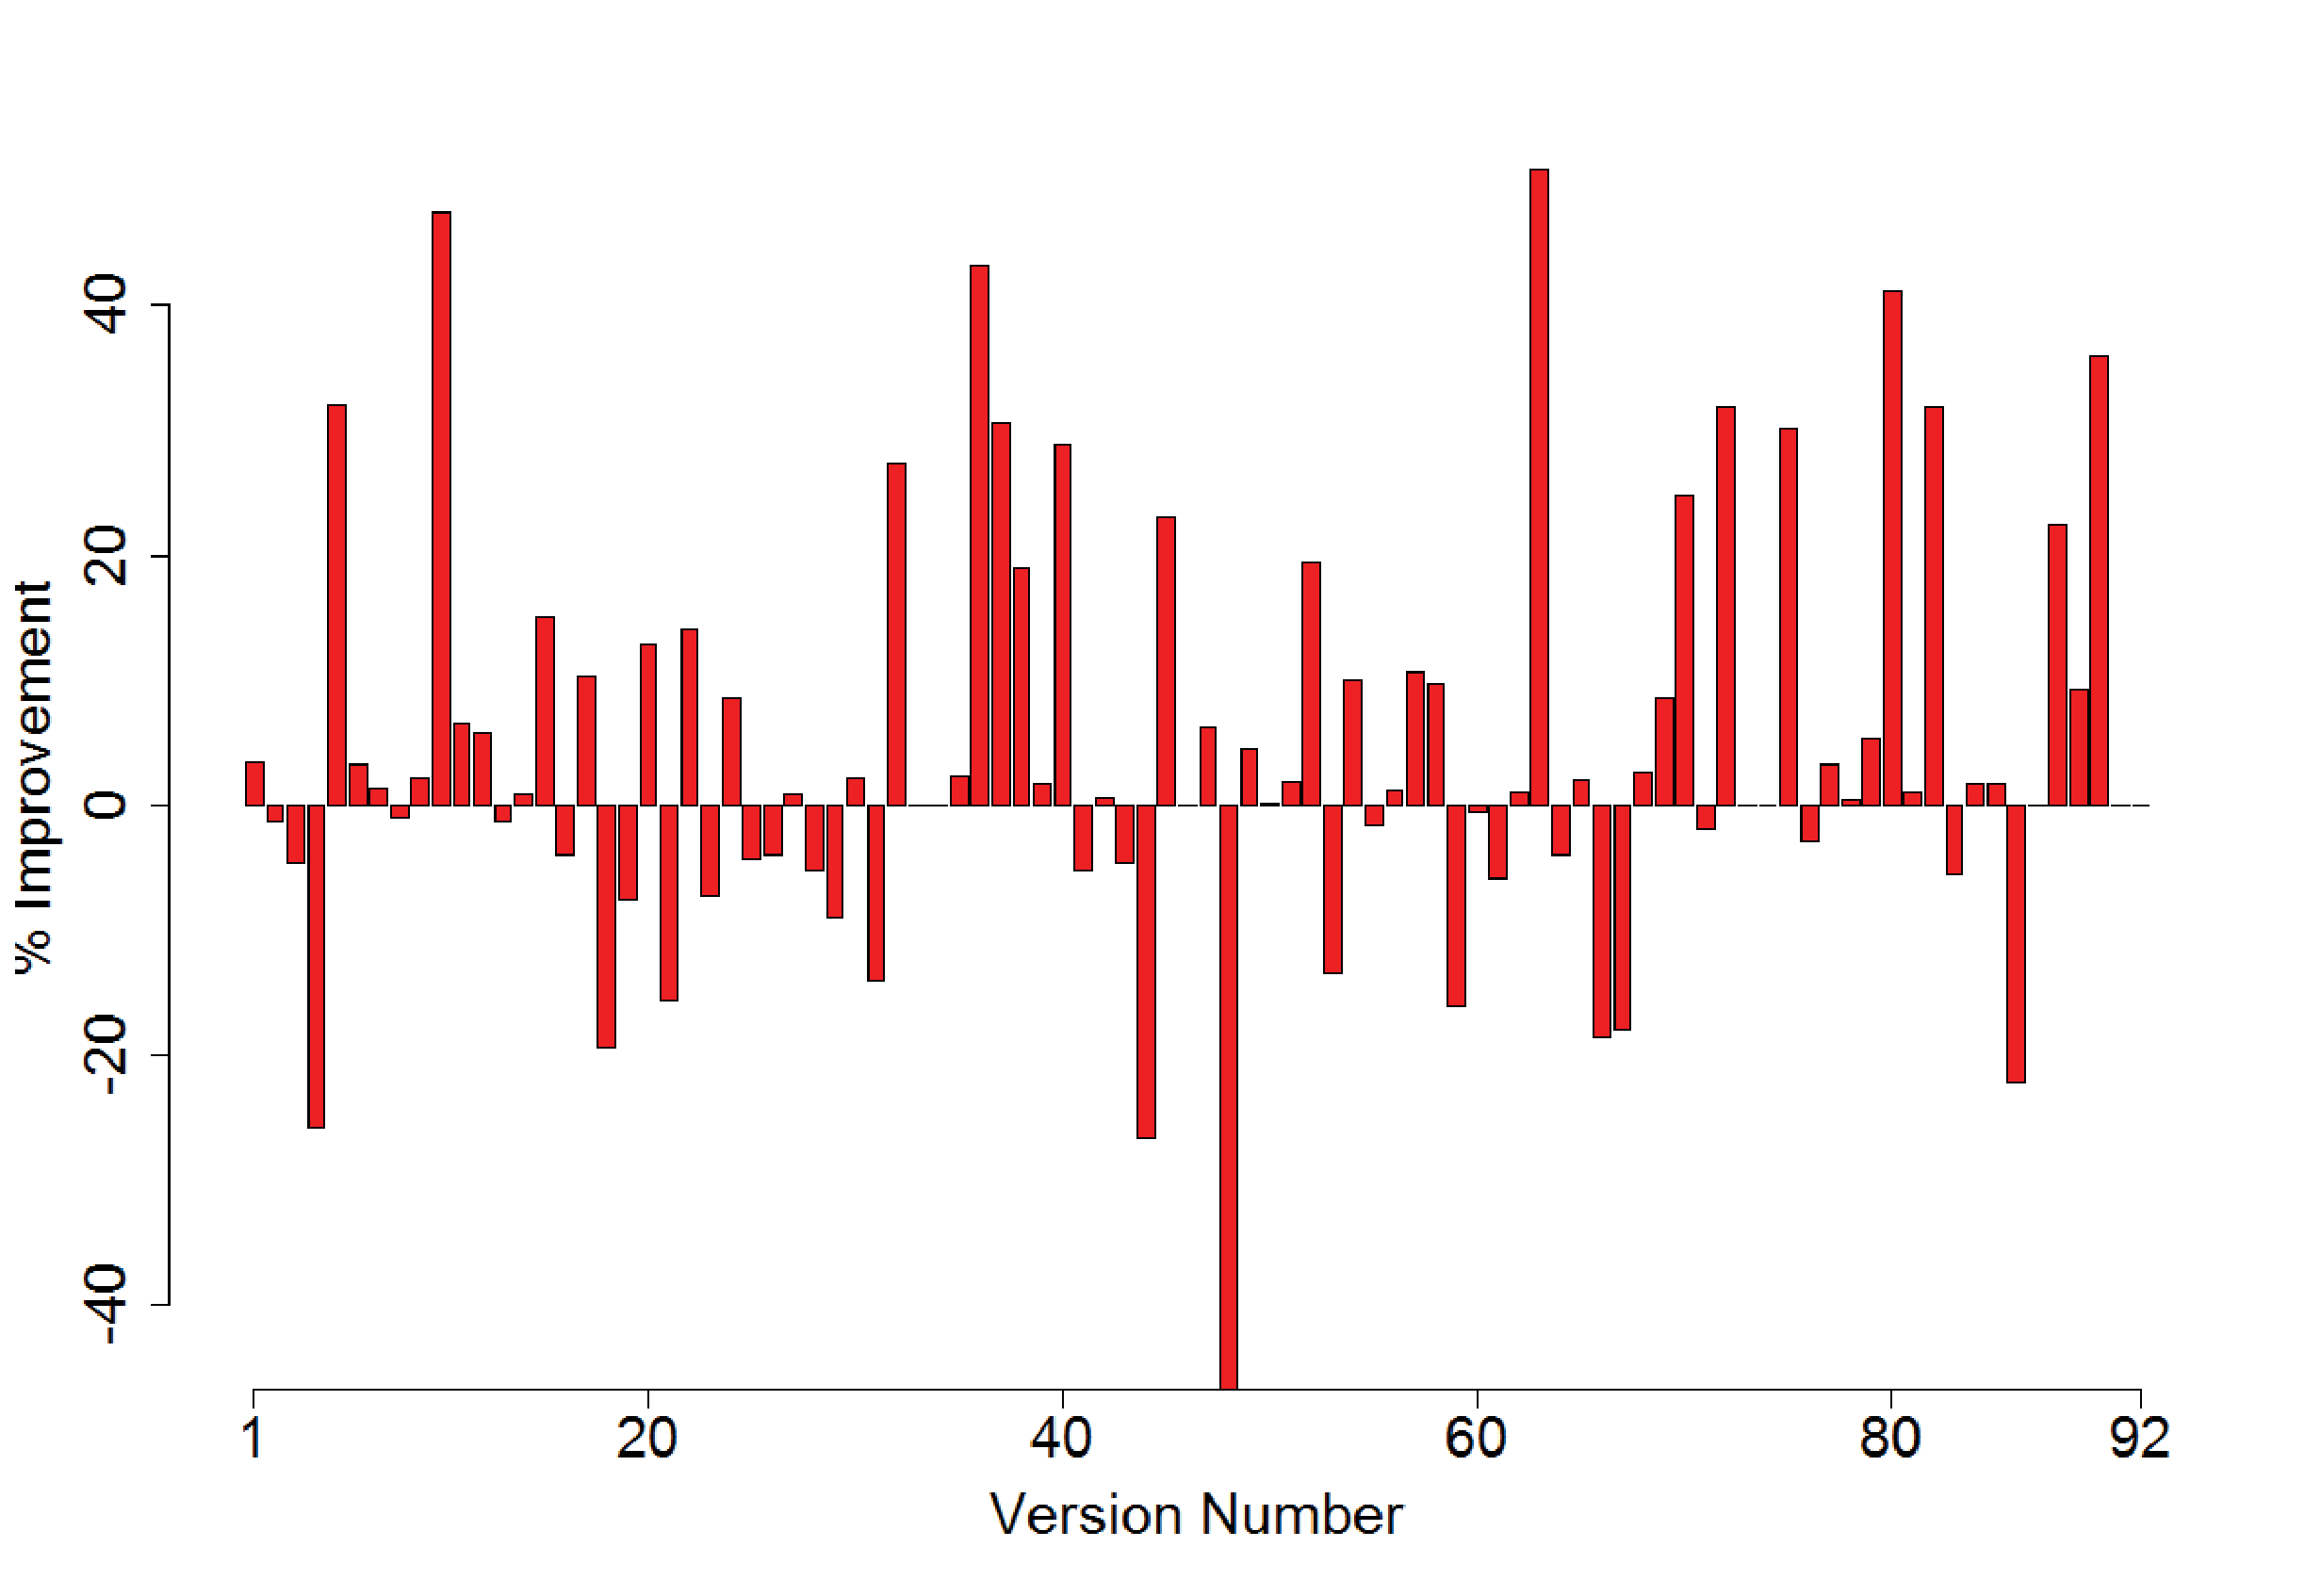
\includegraphics[width=\textwidth]{CBPS_VS_GPS.eps}
\caption{. Relative performance of NUMFL-GPS-QRM and NUMFL-CBPS-QRM on individual single-fault program versions .}
\label{CBPS_VS_GPS}
\end{figure*}

\begin{figure*}[!thpb]
\centering
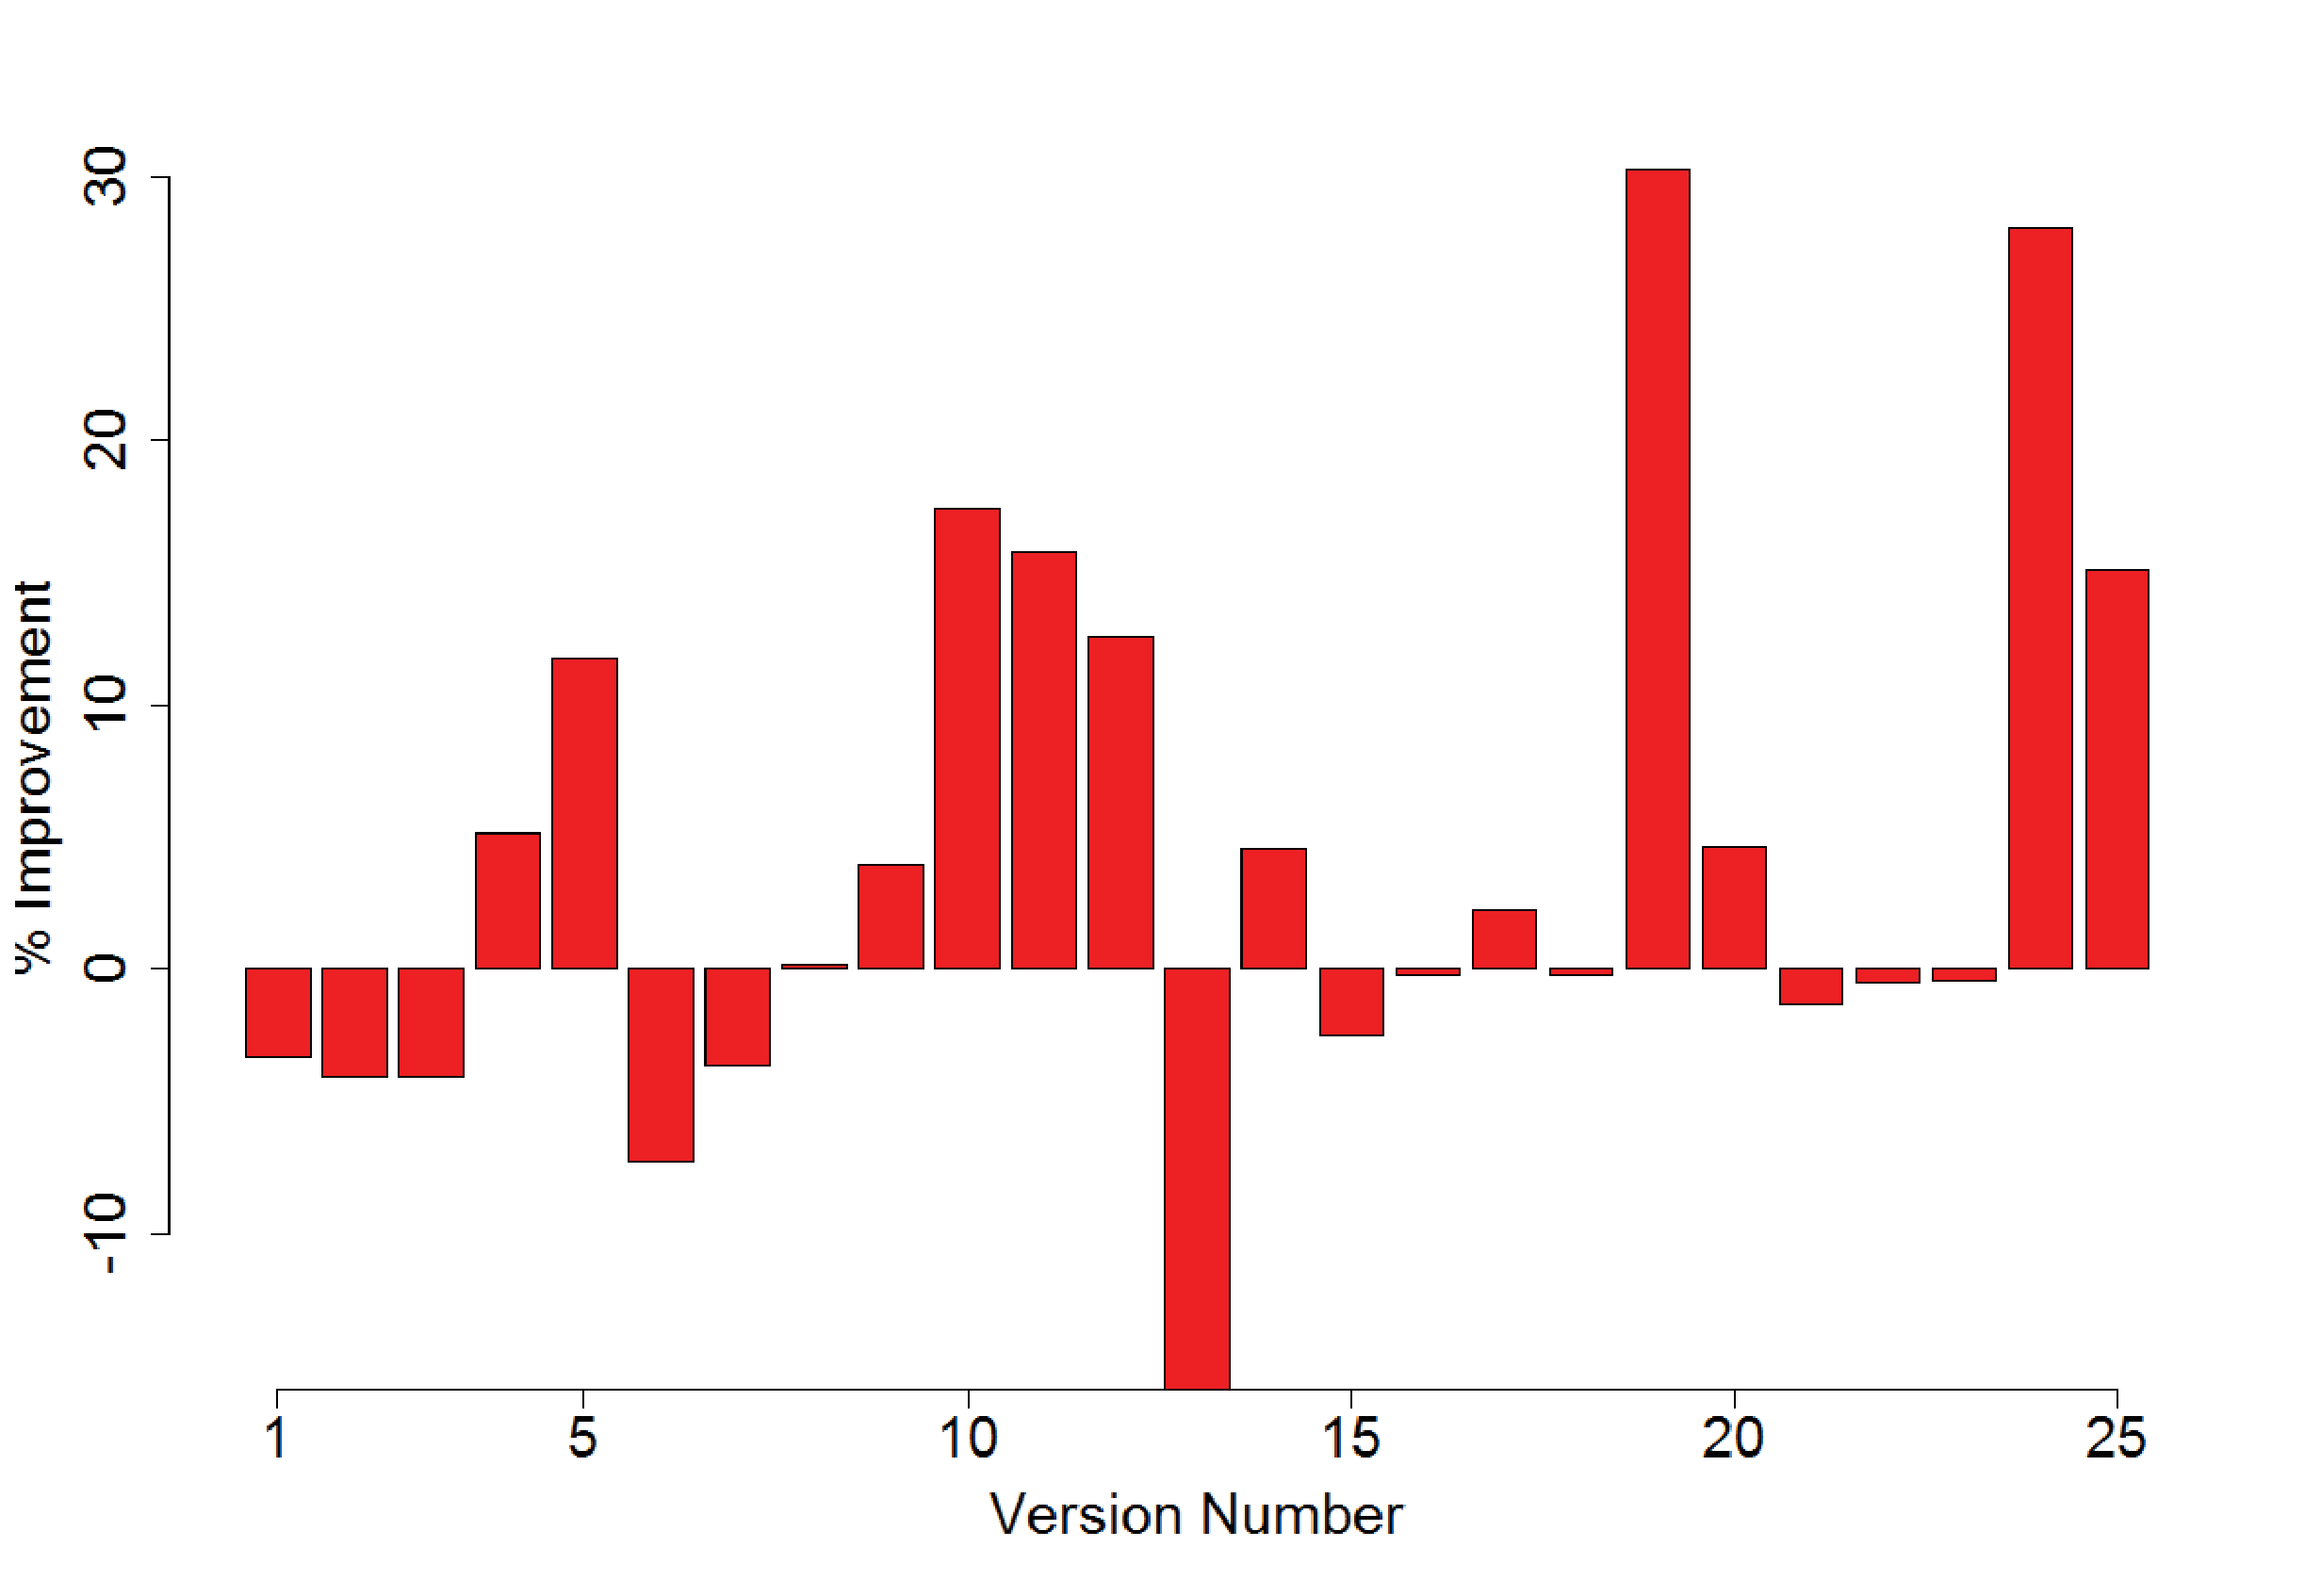
\includegraphics[width=\textwidth]{CBPS_VS_GPS_MultipleFault.eps}
\caption{Relative performance of NUMFL-GPS-QRM and NUMFL-CBPS-QRM on individual two-fault program versions .}
\label{CBPS_VS_GPS_MultipleFault}
\end{figure*}

\subsection{Limitations}
NUMFL and its evaluation are subject to several limitations.  First, NUMFL employs regression models for two purposes: estimating generalized propensity scores and estimating the causal effect of the treatment on the outcome.  We used Gaussian (Normal) linear models for both purposes in NUMFL-GPS, because they are supported by fast and robust software, and they performed well in our empirical study. In NUMFL-CBPS, we use multinomial logistic regression propensity score models.  However, other model choices may be more appropriate for applying NUMFL to different numerical software.  Determining that would require preliminary analysis of the data.  A related issue is that sufficient data must be available to adequately fit each model.  We have found that the number of failing tests should at least 100 to fit adequate regression models.  This is not a serious problem, since faults in numerical programs are usually not guarded by many branch conditions that are likely to cause ``coincidental correctness."  A limitation of our empirical study is that the seeded faults were of three basic types.  In future work, we intend to evaluate NUMFL on subject programs with more varied faults.  Finally, validity of NUMFL (with QRM) depends on Assumptions 1 and 3 in section \ref{twoversion}.  These assumptions do not always hold in practice.  For example, if the effect of a numerical fault does not propagate to the output (coincidental correctness), then Assumption 3 will be violated.

\section{RELATED WORK}\label{relatedwork}
The seminal SFL research of Jones et al. \cite{Jones2002}, which is coverage based, and of Liblit et al. \cite{Liblit2005}, which is predicate based, has inspired much subsequent research.  The use of causal inference methodology in SFL is due to Baah et al. \cite{Baah2010}.  They showed that estimating the AFCE of covering a statement $s$ using a linear regression model that adjusts for coverage of the direct control dependence predecessor of $s$ is effective for reducing confounding bias that often distorts fault localization scores.  Later, Baah et al. \cite{Baah2011} extended this work by using covariate matching to control confounding bias involving both control and data dependence predecessors.  More recently, Gore et al. \cite{Gore2012} extended Baah's initial approach by providing a model that reduces what they called ``failure flow confounding bias," which involves predicate outcomes.  Recently, Shu et al. \cite{Shu2013} proposed a method-level causal inference model to localize faulty methods in large programs. The aforementioned techniques, unlike NUMFL, do not use values of program variables in fault localization.

State-altering techniques, such as {\it cause-transitions} \cite{Cleve2005} and {\it value replacement} \cite{Jeffrey2008} are among the few fault localization techniques based on values of variables.  Cause-transitions employs {\it delta debugging} \cite{Zeller2002} to isolate the cause of a program failure. Value replacement localizes faults by switching program states and re-running the program. Unlike SFL techniques, these techniques actually alter program states, and they require an oracle to determine if alterations cause program failures. On the other hand, they are non-statistical and do not require a sample of both passing and failing executions. The {\it Daikon} system identifies possible invariant conditions in a program based on a sample of executions \cite{Ernst2007}. The {\it DIDUCE} system uses Daikon to report violations of dynamic invariants, which may indicate failures \cite{Hangal2002}. However, these techniques do not address confounding bias.


Some recent studies have developed techniques to analyze instability in floating-point computations. {\it CADNA} \cite{Scott2007} is a library to estimate round-off errors with Monte-Carlo Arithmetic. Tang et al. \cite{Tang2010} proposed a technique to automatically detect such errors by systematically altering the underlying numerical calculation. Lam et al. \cite{Lam2013} proposed to use the detection of significant digit cancellation events to test the precision of numerical programs.  Later, Zhang et al. \cite{Bao2013} extended Lam's work by monitoring the propagation of cancelled bits.  These studies focused on detecting accumulated round-off errors due to finite-precision computation, but they do not address the problem of localizing faults in numerical expressions generally.


Other researchers have proposed alternatives to Imai and van Dyk's approach to defining and using the generalized propensity score.  Hirano and Imbens estimate the causal effect of a continuous treatment variable by fitting one regression model with the GPS as a predictor \cite{Hirano2004}. This method requires discretizing the treatment variable when calculating the propensity score.  Zhao and Imai extend Hirano and Imbens's work by using a smooth coefficient model (SCM) in the regression, so the model can estimate the dose-response function of the treatment variable instead of average causal effect \cite{Zhao2013}.  In preliminary work (with different subject programs), we found that these GPS methods did not perform as well as Imai and Van Dyk's approach, which is used in this paper.


\section{CONCLUSION}\label{conclusion}
In this chapter, we have presented and evaluated a value-based causal model, denoted NUMFL, for localizing faults in numerical software. NUMFL employs generalized propensity scores and covariate balancing propensity scores to control confounding bias involving floating-point program variables that carry erroneous values to correct statements.  NUMFL uses a quadratic regression model (QRM) to estimate the average failure-causing effect of a numerical expression.  We reported the results of an empirical comparison of NUMFL to several competing techniques on both single-fault subject programs and multiple-fault subject programs.  NUMFL performed notably better than the other techniques. We also found that NUMFL-GPS works well with data from failing {\it runs alone}.  Finally, we compared the performance two versions of NUMFL, denoted NUMFL-GPS and NUMFL-CBPS, based on the two aforementioned types of propensity scores. We found that the NUMFL-GPS performed better than NUMFL-CBPS for both single-fault programs and two-fault programs.   In the future work, will seek to extend our empirical results to a broader range of subject programs with more varied fault types.  We intend eventually to evaluate NUMFL in a user study, but given the difficulty of conducting an unbiased one, we think it is desirable to refine NUMFL as much as possible beforehand.  Finally, we will also explore the integration of NUMFL with coverage or predicate based causal SFL techniques. 
\chapter{Causal Inference Based Fault Localization for Numerical Software with Bayesian Additive Regression Trees}\label{chap:BART}


\section{Introduction}\label{BARTintro}
\vspace{-2pt}
Average failure causing effect estimation is challenging when the outcome $Y$ is not linearly related to the treatment $T$ and confounders $X$. Previous work like NUMFL estimates AFCE with non linear parametric regression model \cite{bai2015numfl}, which depends on some pre-assumptions of the relationship between $T$ and $Y$, given the confounding variable $X$ is well controlled.  If any assumption does not hold, then the AFCE estimation can be biased. Bayesian Additive Regression Trees(BART), a new causal effect estimation method has been proposed in the past few years. It is requires less guess-work in model fitting and handles the large number of predictors.
  
In this chapter, we proposal a new statistical fault localization method based on BART model and evaluate it on numerical programs with single or multiple faults. The motivation for using BART in statistical fault localization is:
\vspace{-0.2cm}
\begin{itemize}
\item BART can flexibly fit non-linear response surfaces even with a large number of predictors
\item BART does not require the researcher to specify the functional form of the relationship between treatment and outcome. The user only need to input the treatment, confounding variable and the outcome, but not need to provide how these variables are parametrically related. Also, comparing to methods such as propensity score matching and subclassification, BART produces coherent posterior predictions.
\item The casual inference techniques has been proved to be effective in both coverage based fault localization and value based fault localization. The treatment effect estimated with BART appear to be substantially more accurate than linear regression, and propensity score matching with regression adjustment when the treatment variable is binary. It has potential in estimating failure-causing effect for continuous treatment \cite{hill2012bayesian, hill2013assessing}.
\item BART algorithm software is freely available and easy to use \cite{BARTMachine}.
\end{itemize}

The rest of the chapter is organized as follows: we present the background of single regression tree and BART model in Section \ref{BARTbg}; Using BART model to estimate failure-causing effect is described in detail in Section \ref{BARTafce};  we report on its empirical evaluation in Section \ref{BARTevaluation}; related work is surveyed in Section \ref{BARTrelatedwork}; and Section \ref{BARTconclusion} concludes the chapter.

\section{BART Model Algorithm}\label{BARTbg}%what is BART and why BART
The BART model algorithm consists of three parts: a sum of regression trees model, a regularization prior and a fitting algorithm Marcov Chain Mote Carlo (MCMC)
\subsection{A Single Regression Tree model}\label{IIIA}
Regression tree is one type of decision tree that predicts the value of a target variable based on several input variables. Regression tree handles the situation when the target variable is continuous. Figure \ref{singlergt} shows a single regression tree model. All the interior nodes of a regression tree have decision rules which send the input data set to either left or right side. After the input data set go through the interior nodes and reach the bottom of the tree, the data set is divided into several disjoint subgroup. Each group of data is represent by a leaf node.

\begin{figure*}[!thpb]
\centering
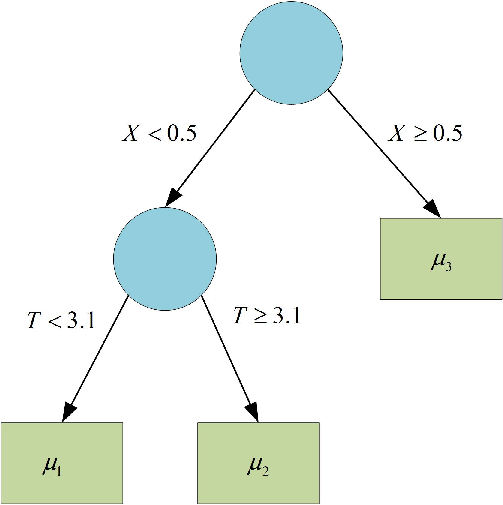
\includegraphics[width=0.5\textwidth]{chapter4_SingleRGT.pdf}
\caption{Single Regression Tree Structure}
\label{singlergt}
\end{figure*}

A single regression tree model is denoted as:
\begin{equation*}
Y=g(\pmb{Z}; R, M)+\epsilon
\end{equation*}
Here $\varepsilon  \sim N(0,{\sigma ^2})$ is a normal distributed error .$\pmb{Z}=[T,\pmb{X}]$ denotes all the variables related to the outcome $Y$, so $Z$ includes both treatment variable $T$ and confounding variables $\pmb{X}$. $R$ denotes a binary regression tree consisting a set of interior node decision rules and a set of terminal nodes, and let $M=
\begin{Bmatrix}
 \mu _1, \mu _2, . . ., \mu _b
\end{Bmatrix}$
denotes a set of parameter value associated with each of the $b$ terminal nodes of $R$. Each terminal node represent a regression model of outcome $Y$ on all the variables $Z$.

A regression tree model is often used in approximating unknown functions. For example, if the causal effect of treatment $T$ on outcome $Y$ is decided by an unknown function $Y=f(T,\pmb{X})$, then we can approximate the function $f(T,\pmb{X})$ by fitting a single regression tree model g(\pmb{Z}; R, M) on sample data set. The regression tree model divides the value space of $[T,\pmb{X}]$ in to several subgroups with its tree structure and fit a regression model for each subgroup. When making inference of $Y$ given a specific unit of treatment and confounding variables values $[T=t,\pmb{X}=\pmb{x}]$, the regression will first find out which subgroup the unit belongs to and then infer outcome $Y$ with the corresponding linear regression. Regression tree model has two advantages: (1) making prediction is fast. (2) it can handle non-linear function approximation.


\subsection{A sum of regression trees model}
BART model is a sum of trees model. With the definition of a single tree model, the sum of trees model can be expressed as:
\begin{equation*}
Y = g(\pmb{Z};{R_1},{M_1}) + g(\pmb{Z};{R_1},{M_1}) +  \cdots  + g(\pmb{Z};{R_m},{M_m}) + \varepsilon
\end{equation*}
where each $(R_i,M_i)$ denotes a single sub-tree model and $\varepsilon  \sim N(0,{\sigma ^2})$.  $m$ denotes the number of trees in BART model. We have
 \begin{equation*}
 Y =f(\pmb{Z})=f(T,\pmb{X})= \left( {\sum\limits_{j = 1}^m {g(T,\pmb{X};{R_j},{M_j})} } \right) + \varepsilon
 \end{equation*}

Comparing to single regression tree model, BART model has two advantages. First BART is more naturally handle the interaction effects . In the sum of trees model, each tree explains part of the overall fit, so there are many different choices of $(R_1,M_1) \cdots (R_m,M_m)$ can lead to an identical function$ \sum\limits_{j = 1}^m {g(T,\pmb{X};{R_j},{M_j})} $. Second, BART can scale to large datasets using a parallel MCMC sampler \cite{pratola2014parallel, pratola2015bayesian}. Thus, fitting BART model does not has much more computation cost than fitting a large single tree model.

\subsection{A regularization prior}
Fitting the BART model requires a prior of all the parameters of the sum of trees model.  The prior regularize the fit by keeping the individual tree's effect from being unduly influential. Without such a prior, large  tee components would dominate the sum of trees structure. The regularization prior can also help BART avoid overfitting. To simplify the prior specification, the trees in BART model $(R_1, M_1), (R_2,M_2), \ldots, (R_m, M_m) $ are considered to be independent of each other and of $\sigma$. Also, the terminal node parameters $ \mu _{1j}, \mu _{2j}, . . ., \mu _{bj} $ of every tree $R_j$ are independent. So we have:

\begin{equation*}
 \begin{array}{l}
P(({R_1},{M_1}),({R_2},{M_2}) \ldots ,({R_m},{M_m}),\sigma ) = \left[ {\prod\limits_j {P({R_j},{M_j})} } \right]p(\sigma )\\
\quad \quad \quad \quad \quad \quad \quad \quad \quad \quad \quad \quad \quad \quad \; = \left[ {\prod\limits_j {P({M_j}|{R_j})P({R_j})} } \right]p(\sigma )
\end{array}
 \end{equation*}
and
\begin{equation*}
P({M_j}|{R_j}) = \left[ {\prod\limits_i {P({\mu _{ij}}|{R_j})} } \right]
 \end{equation*}
Here ${\mu _{ij}} \in {M_j}$ denotes the $ith$ terminal node of the $jth$ regression tree From the above equations, we can see the independence simplify the prior specification problem to the specification of prior for just ${P({\mu _{ij}}|{R_j})}$, $P({R_j})$ and $P(\sigma)$. In \cite{chipman2010bart}, the specification of prior forms on $P(\sigma)$ is defined as the inverse chi-square distribution. The prior on ${P({\mu _{ij}}|{R_j})}$ is defined as conjugate normal distribution. The prior on $P(R_j)$ is complicated which contains 3 aspects:
\begin{enumerate}
\item the probability that a nonterminal node at depth $d$ is given by
\begin{equation*}
\alpha {(1 + d)^{ - \beta }},\quad \alpha  \in (0,1),\beta  \in [0,\infty )
 \end{equation*}
\item the prior probability that a variable is selected as the splitting variable at an interior node is $1/k$ and $k$ is the total number of variables including both treatment and confounders.
\item the prior probability that a splitting variable split at value $x$ is $1/N$ and $N$ is the total number of observed values of the splitting variable in the sample data set.
\end{enumerate}
The detail of the prior specification for ${P({\mu _{ij}}|{R_j})}$, $P({R_j})$ and $P(\sigma)$ can be reffered to \cite{chipman2010bart}.


\subsection{Bayesian Backfitting MCMC Algorithm}
BART uses a Bayesian backfitting  MCMC algorithm to fit the model \cite{gilks2005markov}. The algorithm uses Gibbs sampler \cite{casella1992explaining}. The Gibbs sampler get $m$ successive draws of $(R_j, M_j)$ conditionally on $(R_{(j)}, M_{(j)}, \sigma)$:

\begin{equation*}
(R_j,M_j)|R_{(j)}, M_{(j)}, \sigma, Y
\end{equation*}
$j=1 \ldots m$, followed by a draw of $\sigma$ from the full conditional:

\begin{equation*}
\sigma |{R_1}, \ldots ,{R_m},{M_1}, \ldots ,{M_m},Y
\end{equation*}
Here $R_{(j)}$ represents all the trees except $R_j$, so $R_{(j)}$ will be a set of $m-1$ trees. $M_{(j)}$ is similarly defined as $R_{(j)}$.

\section{BART Model with Causal Inference}\label{BARTafce}% how to use BART

When apply BART model in estimating average causal effects, we use different algorithms for binary treatment and continuous treatment. For binary treatment, BART model primarily estimate failure-causing effects such as $E(Y(1)|\pmb{X}=\pmb{x}) - E(Y(0)|\pmb{X}=\pmb{x})=E(Y|T=1, \pmb{X}=\pmb{x})-E(Y|T=0, \pmb{X}=\pmb{x})=f(1,\pmb(x))-f(0,\pmb(x))$ . The algorithm contains the following steps:
\begin{enumerate}
\item Fit BART model using MCMC algorithm to full sample
\item Get posterior prediction for each unit by setting the treatment variable value $T=1$ and keep confounding variable value unchanged..
\item Get posterior prediction for each unit by setting the treatment variable value $T=0$ and keep confounding variable value unchanged.
\item	Calculate the difference between the posterior predictions for each unit.
\item Estimate failure-causing effect by averaging all the differences of posterior predictions.
\end{enumerate}

In step 1, the fitted BART model characterized the causal relationship between treatment $T$ and outcome $Y$ given the confounding $\pmb{X}$. We can use the fitted model to predict the outcome $Y$ under different $(T, \pmb{X})$ conditions. For a untreated unit $(T=0, \pmb{X}=\pmb{x})$,  if we set the treatment variable to 1 and then input $(T=1, \pmb{X}=\pmb{x})$ into the BART model, the output is the estimated outcome for that unit in treated condition. Similarly, we can estimate the outcome of a treated unit in untreated condition by inputing $(T=0, \pmb{X}=\pmb{x})$ into the BART model. Thus, in step2, the BART model is used to predict outcome for each unit at observed treatment condition. In step 3, the fitted BART model is used to estimate posterior predictions for each unit at counterfactual condition. Thus, the difference calculated in step 4 is the causal effect estimation for each unit. The average of these differences is failure-causing effect causal effect which is estimated in step 5.

If the treatment variable is continuous, the causal effect of treatment $T$ on outcome $Y$ is characterized by a function $r_e (T)$, which is called dose-response function in medical research. For the failure-causing effect, the dose response functions of continuous treatments are usually non-linear. For example, in Chapter 3, NUMFL use parameterized quadratic model and double linear model to approximate the dose response function within subclasses and get reasonable well result. But the parameterized model has limitations. It usually requires user to make assumptions to specify form of the dose-response function.  For example, in NUMFL, we make some assumptions ($Assumptioin 1, 2, 3$).  The  $Assumptions3$ is: executions with large absolute treatment errors have larger output errors than executions with small values of treatment errors.  Although this assumption is often holds in numeric programs, it is not always to be true. In this case,  the dose response curve of treatment $T$ on outcome $Y$ is likely to deviate from the quadratic model $Y = \zeta {T_e}^2 + \eta {T_e} + c$, which may result in a bad estimation of failure-causing effect. Comparing to parametric model used in NUMFL, BART model does not require user to make assumptions or specify the functional form of the dose response function. The sum of trees structure of BART model can approximate the non-linearity of the DRF during the training phone with MCMC.

failure-causing effect estimation is a challenge for BART model. In NUMFL, the failure-causing effect is characterized by the coefficient of the regression model.  But in BART model, the sum of trees structure does not such parameters can directly characterize the ACE. To solve this problem, we propose to estimate the treatment causal effect at each unit in the sample. The average of the treatment causal effect on all sample units is the estimated ACE. The causal effect of treatment T on outcome Y for a single unit can be estimated by increasing the treatment variable value of the unit and see how outcome changes. For example, assume a unit $i$ has treatment variable $T=t$ and confounding variables$\pmb {X}=\pmb {x}$, we can use the fitted BART model to estimate the outcome of the unit $Y=y$. Then we increase the treatment variable to $t'=t+\varepsilon$, here $\varepsilon $ is a small number. We input $T'$ and $\pmb{X}$ into the fitted BART model and get the estimated posterior $Y=y'$. Then the estimated causal effect of $T$ on $Y$ for unit $i$ is $\left| {y - y'} \right|$. The algorithm is as follows:
\begin{enumerate}
\item Fit BART model using MCMC algorithm to full sample
\item Increase the treatment variable value $t$ of each unit by $\varepsilon $. The new treatment value $t'=t+\varepsilon$ and the original confounding variables forms a new data set.
\item For each unit, calculate the difference between the posterior prediction in original data set and the posterior prediction in the new data set.
\item Estimate failure-causing effect by averaging all the differences of posterior predictions.
\end{enumerate}

In the above algorithm, the BART model fitted in first step is used to approximate a function $Y=f(T,\pmb(X))$ that specify the dose-response function of the continuous treatment $T$ and confounding variables $\pmb{X}$. Step 2 and Step 3 estimate the treatment causal effect for each sample unit. Step 4 estimate the failure-causing effect of treatment on outcome.

One problem in step 2 is how to choose the value of the small number $\varepsilon $. But treatment variables in different numerical expressions have different scale of values, it is hard to find a constant $\varepsilon$ which can make $t+\varepsilon$ be a reasonable value for all the treatments. To address this problem, we use the method illustrated by Figure\ref{bartace}.  We sort the original sample data set shown in Figure\ref{bartace} (a) in increasing order according to the value of the treatment variables.  The sorted data set is shown in Figure\ref{bartace} (b). The increased treatment variable value $t'$ in step 2 is equal to the treatment variable value $t$ of the next unit in the list and the last unit in the list will be discarded. Thus, as shown in Figure ref{bartace} (c), for a data set with $n$ observational units, we will have a new data set of $n-1$ units after increasing the treatment variable. The idea behind this method is that we want the value of treatment after increment is a reasonable value that could be observed in  other tests. Also, the value of $t'$ and the value of $t$ are likely to be in the same scale, because they are neighbor in the sorted data set.

\begin{figure*}[!thpb]
\centering
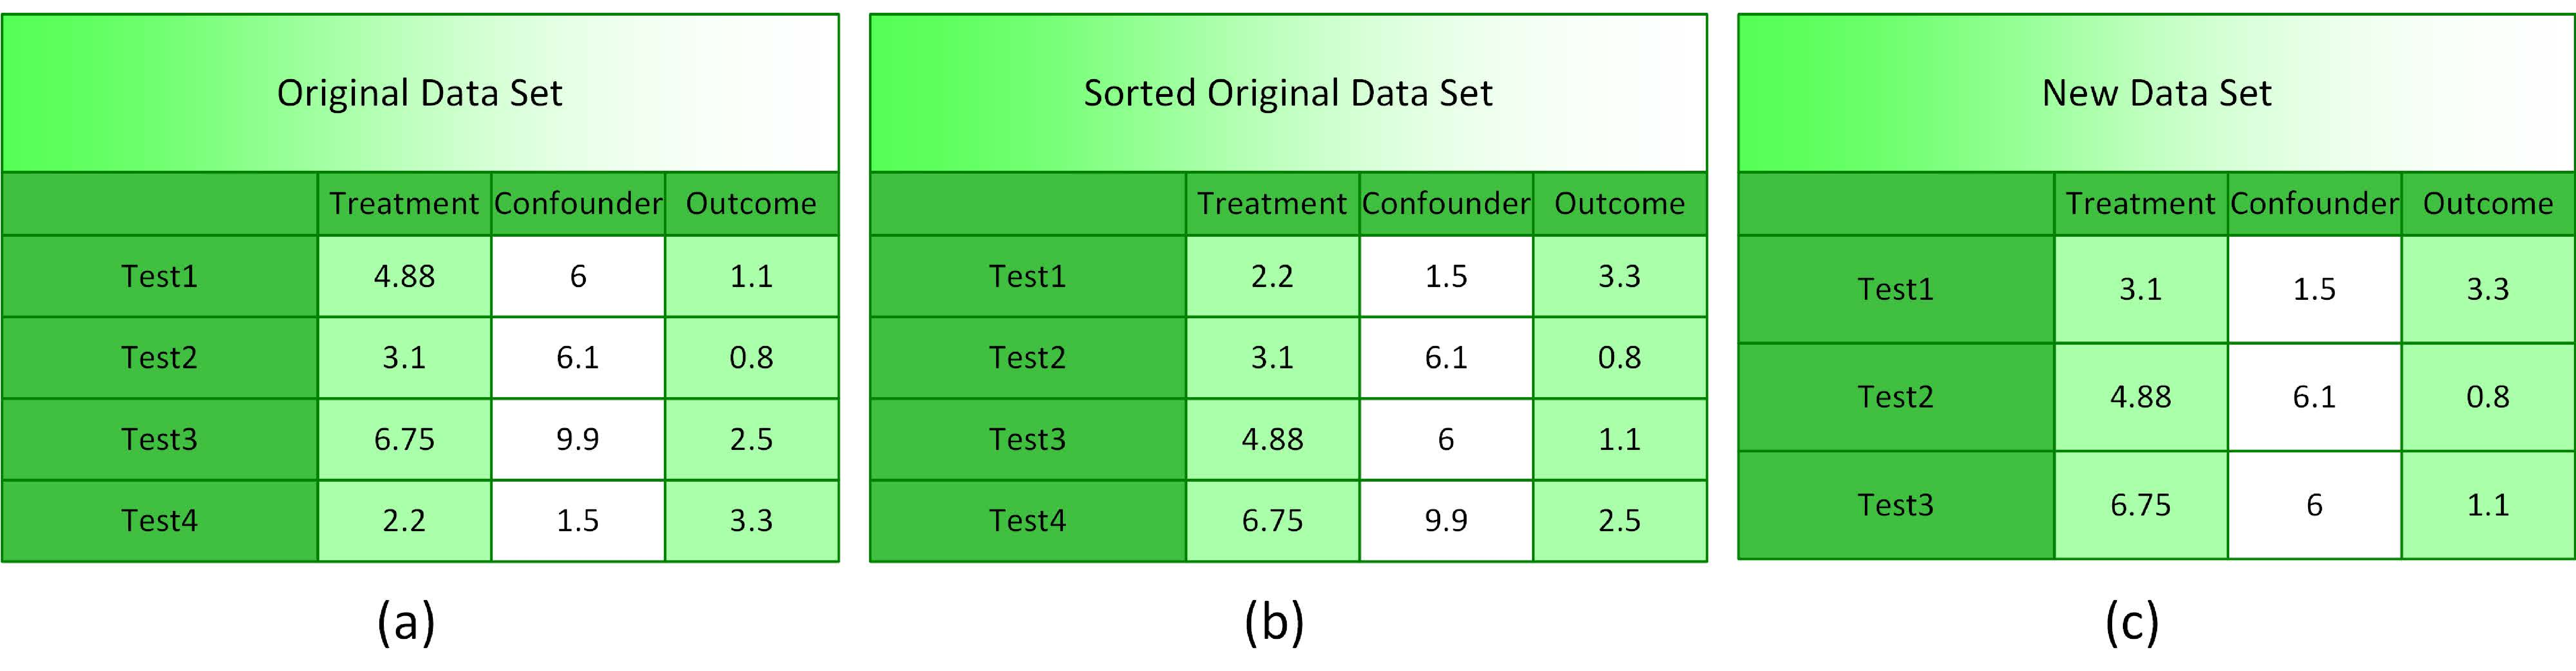
\includegraphics[width=1\textwidth]{chapter4_BART_ACE.pdf}
\caption{EXAMPLE OF TREATMENT VARIABLE INCREAMENT}
\label{bartace}
\end{figure*}

\section{EMPIRICAL EVALUATION}\label{BARTevaluation}% result

To evaluate the effectiveness of BART model, we conducted the empirical study on the same subject programs as described in chapter 3.  The tests suite is also identical to the tests suite in section \ref{numfl_evaluation}.  Overall 92 faulty subject-programs versions with single fault and 25 faulty subject-program versions with two faults. Ochiai, Dstar, SOBER, ESP-SIV are ESP-SCP used as the base line techniques to be compared with BART model. We also compare the performance of BART model with NUMFL-GPS and NUMFL-CBPS which are the proposed in chapter 3. We measured the costs of applying CBPS and the other metrics by the percentage of {\it subexpressions} that need to be examined, in decreasing order of suspiciousness scores, to find the fault, assuming the fault is recognized when it is encountered.

In the experiment, we use R package "BARTMachine" \cite{BARTMachine} to fit the BART model. We tried 10 trees and 50 trees in the sum of trees structure.  The BART model is fitted with both passing and failing tests. The number tests for each subject program is from 3000 to 8000 which shown in table \ref{subpro}. We also try to train BART model with fewer data(300 tests). the sensitivity of the BART model to the number of trees and the number of tests are discussed in section \ref{BARTsensitivity}.

\subsection{Comparative Performance of BART vs. Baselines}

Figure \ref{QRM_VS_Base} shows the results of comparisons of BART with each of the baseline metrics.  In each graph, the vertical axis represents the percentage improvement (reduction) in cost. The horizontal-axis represents different subject-program versions for which there are cost differences between the metrics, with each version represented by a vertical bar.   Bars above the zero-line represent versions for which BART performed better than the baseline metric and bars below zero represent versions for which BART performed worse.  The length of each bar represents the magnitude of the corresponding cost difference.

\textit{\textbf{ BART vs. Ochiai.}}  Over all 92 faulty subject-program versions, BART performed better than the Ochiai metric on 75 versions but BART performed worse on 17 versions.  There were 41 versions for which BART performed at least 20\% better than the Ochiai metric.  There were just 4 versions for which the latter performed better than BART.

\textit{\textbf{ BART vs. DStar.}}  BART performed better than DStar on 77 subject-program versions but BART performed worse than DStar on 15 versions.  BART performed at least 20\% better than DStar on 44 versions, whereas DStar performed at least 20\% better than BART on just 4 versions.

\textit{\textbf{ BART vs. ESP-SIV.}} BART performed better than ESP-SIV on 78 subject-program versions but BART performed worse than ESP-SIV on 14 versions.  BART performed at least 20\% better than ESP-SIV on 30 versions, whereas ESP-SIV never performed at least 20\% better than BART.

\textit{\textbf{ BART vs. ESP-SCP.}}  BART performed better than ESP-SCP on 75 subject-program versions but BART performed worse than ESP-SCP on 17 versions.  BART performed at least 20\% better than ESP-SIV on 22 versions, whereas ESP-SCP performed at least 20\% better than BART on just 2 versions.

\textit{\textbf{ BART vs. SOBER.}}  BART performed better than SOBER on 73 subject-program versions but BART performed worse than SOBER on 19 versions.  BART performed at least 20\% better than SOBER on 39 versions, whereas SOBER performed at least 20\% better than BART on just 5 versions.

\begin{sidewaysfigure}
\centering
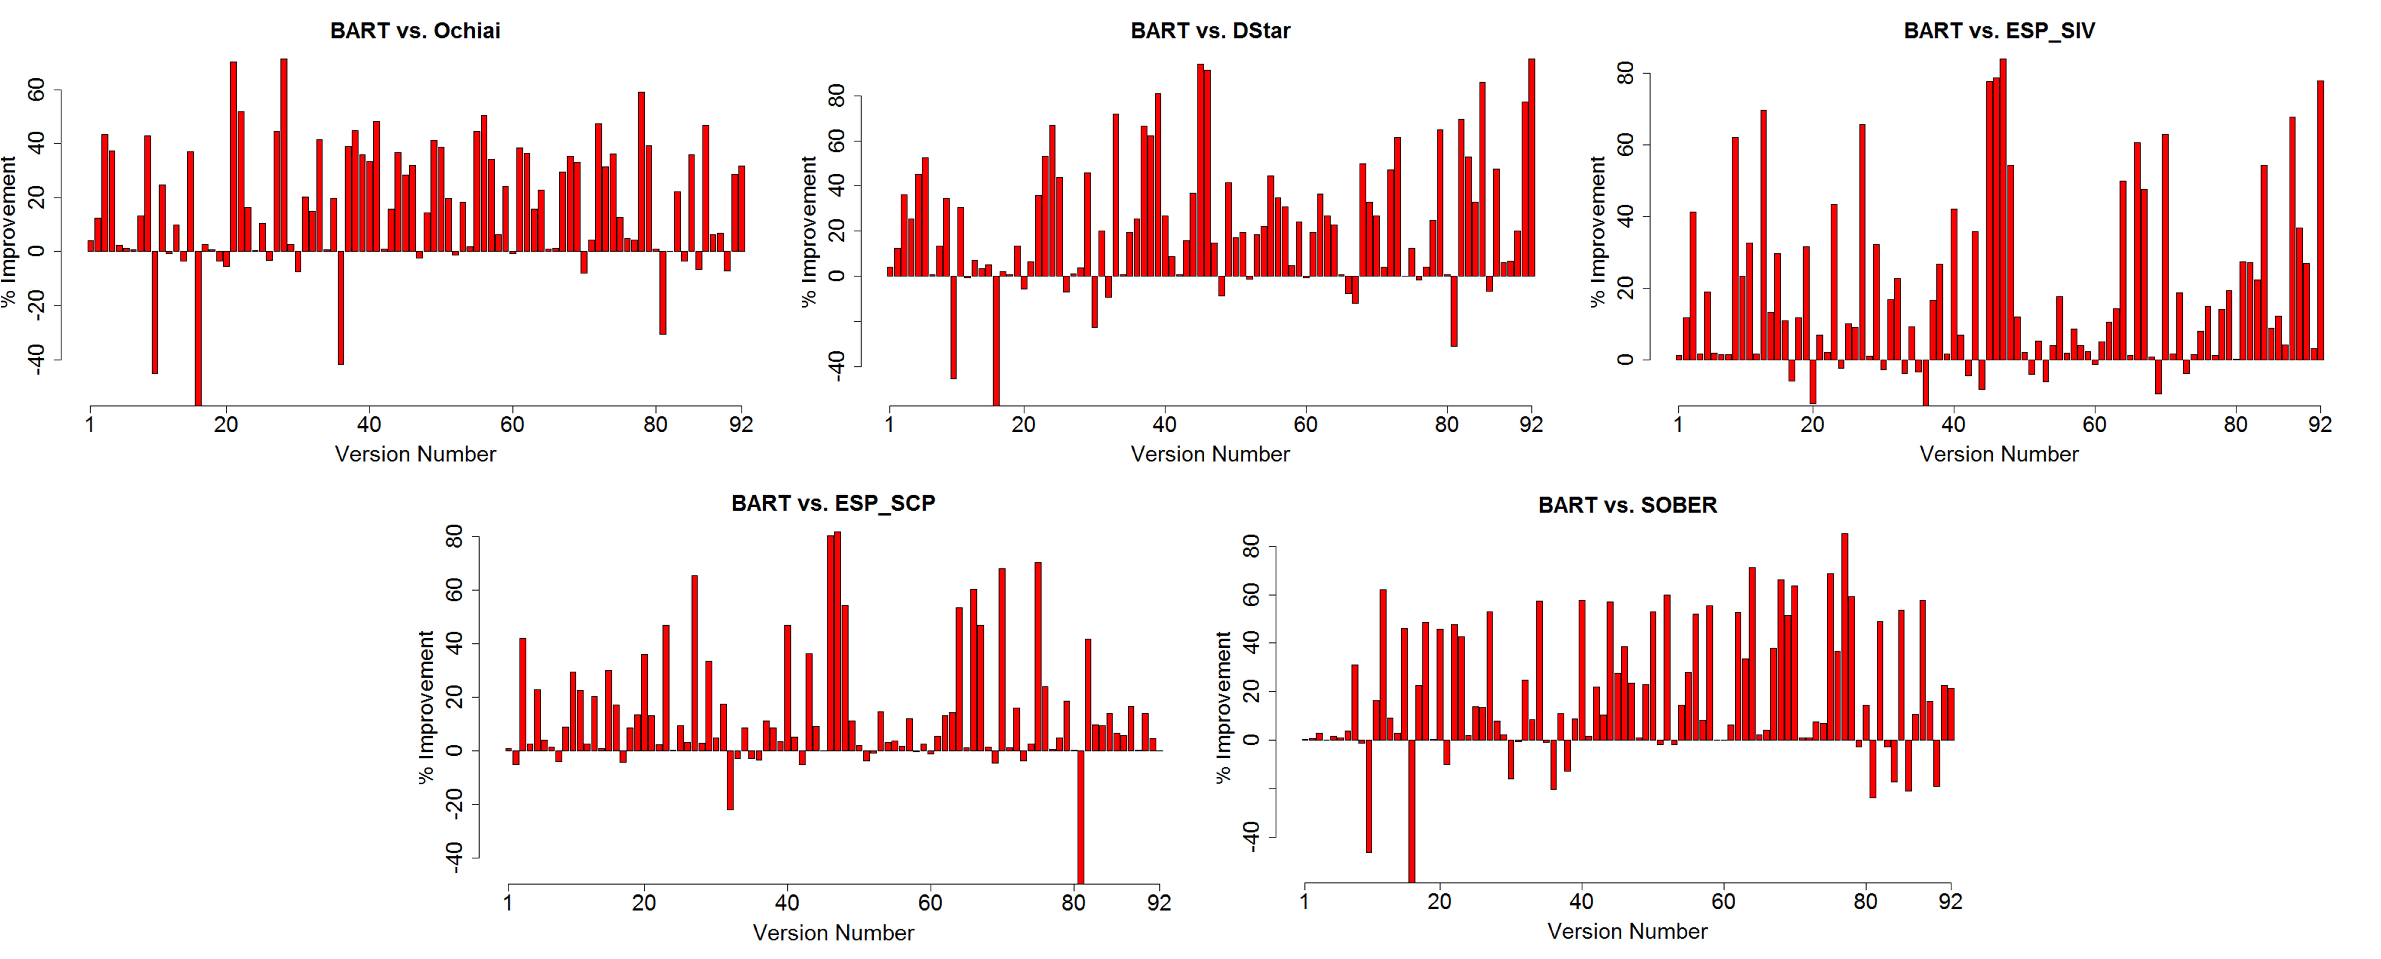
\includegraphics[width=\textwidth]{chapter4_BART_VS_Base.pdf}
\caption{Performance of BART relative to baseline metrics on individual single-fault program versions.}
\label{BART_VS_Base}
\end{sidewaysfigure}

Figure \ref{BART_VS_Base_M} contrasts the performance of BART on the individual two-fault program versions with that of the baseline metrics.  Over all 25 faulty subject-program versions, BART performed better than SOBER on 19 versions but performed worse on 6 versions.  There were 8 versions for which BART performed at least 10\% better than SOBER but 3 versions for which SOBER performed at least 10\% better than BART.  Ochiai performed better than BART on 5 versions but performed worse on 20 versions. BART performed at least 10\% better than Ochiai on 13 versions. BART performed better than both ESP-SIV and ESP-SCP on 20 versions.   BART performed better than DStar on 19 versions.

\begin{sidewaysfigure}
\centering
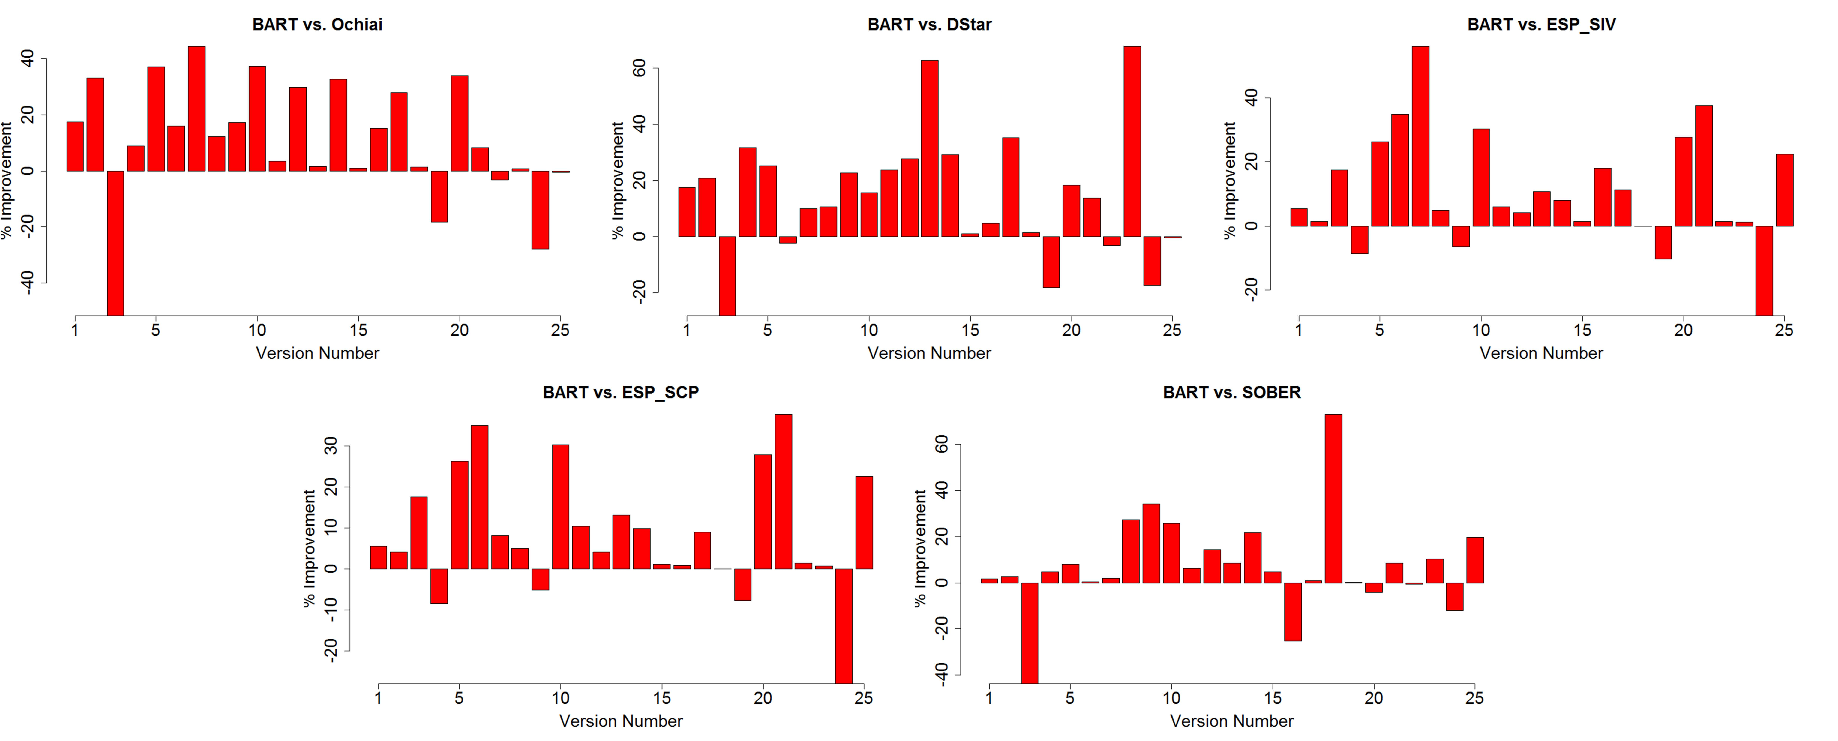
\includegraphics[width=\textwidth]{chapter4_BARTvsBase_M.pdf}
\caption{Performance of BART relative to baseline metrics on individual single-fault program versions.}
\label{BART_VS_Base_M}
\end{sidewaysfigure}


\subsection{BART model vs NUMFL}
Table \ref{tableBARTvsNUMFL} shows the average percentage of subexpressions that had to be examined to find the fault, computed across all the faulty versions, for BART model and NUMFL.  Here we show the results for NUMFL-GPS-QRM and NUMFL-CBPS-QRM.   There were 11 subject programs for which BART performed better than NUMFL-GPS-QRM. There were 5 subject programs for which NUMFL-GPS-QRM performed better than BART. BART performed better than NUMFL-CBPS-QRM on 14 subject programs. There were only 2 subject programs for which NUMFL-CBPS-QRM performed better than BART.

Figure \ref{BARTvsQRM} graphically contrasts the performance of BART and NUMFL-GPS-QRM on the single fault versions.  BART performed better than NUMFL-GPS-QRM on 54 versions, while NUMFL-GPS-QRM performed better on 38 versions.  BART performed at least 20\% better than NUMFL-GPS-QRM on 9 versions, whereas NUMFL-GPS-QRM performed at least 20\% better than BART on 6 versions. Figure \ref{BARTvsCBPS} graphically contrast the performance of BART and NUMFL-CBPS-QRM on the single fault versions.  BART performed better than NUMFL-CBPS-QRM on 61 versions, while NUMFL-CBPS-QRM performed better on 31 versions.  BART performed at least 20\% better than NUMFL-CBPS-QRM on 17 versions, whereas NUMFL-CBPS-QRM performed at least 20\% better than BART on just 4 versions.

In summary, BART  performed better than both NUMFL-GPS-QRM and NUMFL-CBPS-QRM on single-fault programs. This may be due to the fitted sum of trees structure of BART model well approximate the DRF of treatment variable and thus have more accurate average cause effect estimation than NUMFL techiniques.

\begin{table*}[htbp!]
\caption{AVERAGE FAULT LOCALIZATION COSTS OF BART AND NUMFL METRICS ON SINGLE-FAULT PROGRAM VERSIONS}
\label{tableBARTvsNUMFL}
\centering
      \begin{tabular}{|l|c|c|c|}
      \hline
\multirow{2}{*}{Subject Program}	& \multirow{2}{*}{BART}&	\multicolumn{2}{|c|}{{\bf NUMFL}}	\\	\cline{3-4}
& & GPS-QRM	&CBPS-QRM \\ \hline
Apache\_EigenDecompose &	2.50\%&	12.3\%	&	8.8\%	\\	\hline
Apache\_DScompiler&	9.72\%&	11\%	&	12\%	\\	\hline
Apache\_BigMatrix	&	9.00\%&11.4\%	&	9.9\%	\\	\hline
Apache\_Rotation3D&	9.07\%&	8\%	&	18.9\%	\\	\hline
Ojaljo\_SchurDecompose&	10.61\%&	11.4\%	&	14\%	\\	\hline
Jama\_MatrixDecompose	&11.62\%&	14.2\%	&	23\%	\\	\hline
SciMark\_LU&8.33	\%&	15.3\%	&	27.8\%	\\	\hline
SciMart\_FFT&	 27.59\%&	9.5\%	&	19.8\%	\\	\hline
Apache\_SymmLQ&	 1.75\%&	2.6\%	&	4.4\%	\\	\hline
Apache\_SplineInterpolator&	 37.78\%&	31.7\%	&	35\%	\\	\hline
Apche\_SimpleRegress&	 1.70\%&	4.3\%	&	17\%	\\	\hline
Apache\_SchurTransformer&	 4.56\%&	3.3\%	&	14.9\%	\\	\hline
Apache\_MillerUpdatRegress&	 1.24\%&	7.5\%	&	9.9\%	\\	\hline
Apache\_HarmonicFitter&	30.10\%&	27.3\%	&	32\%	\\	\hline
Apache\_FastSine&	1.53\%&	1.5\%	&	13\%	\\	\hline
Apache\_FastCosine	&1.29	\%&1.3\%	&	1.2\%	\\	\hline
Average Cost	&	10.52\%&10.8\%	&	16.4\%	\\	\hline
\end{tabular}
\end{table*}

\begin{figure*}[!thpb]
\centering
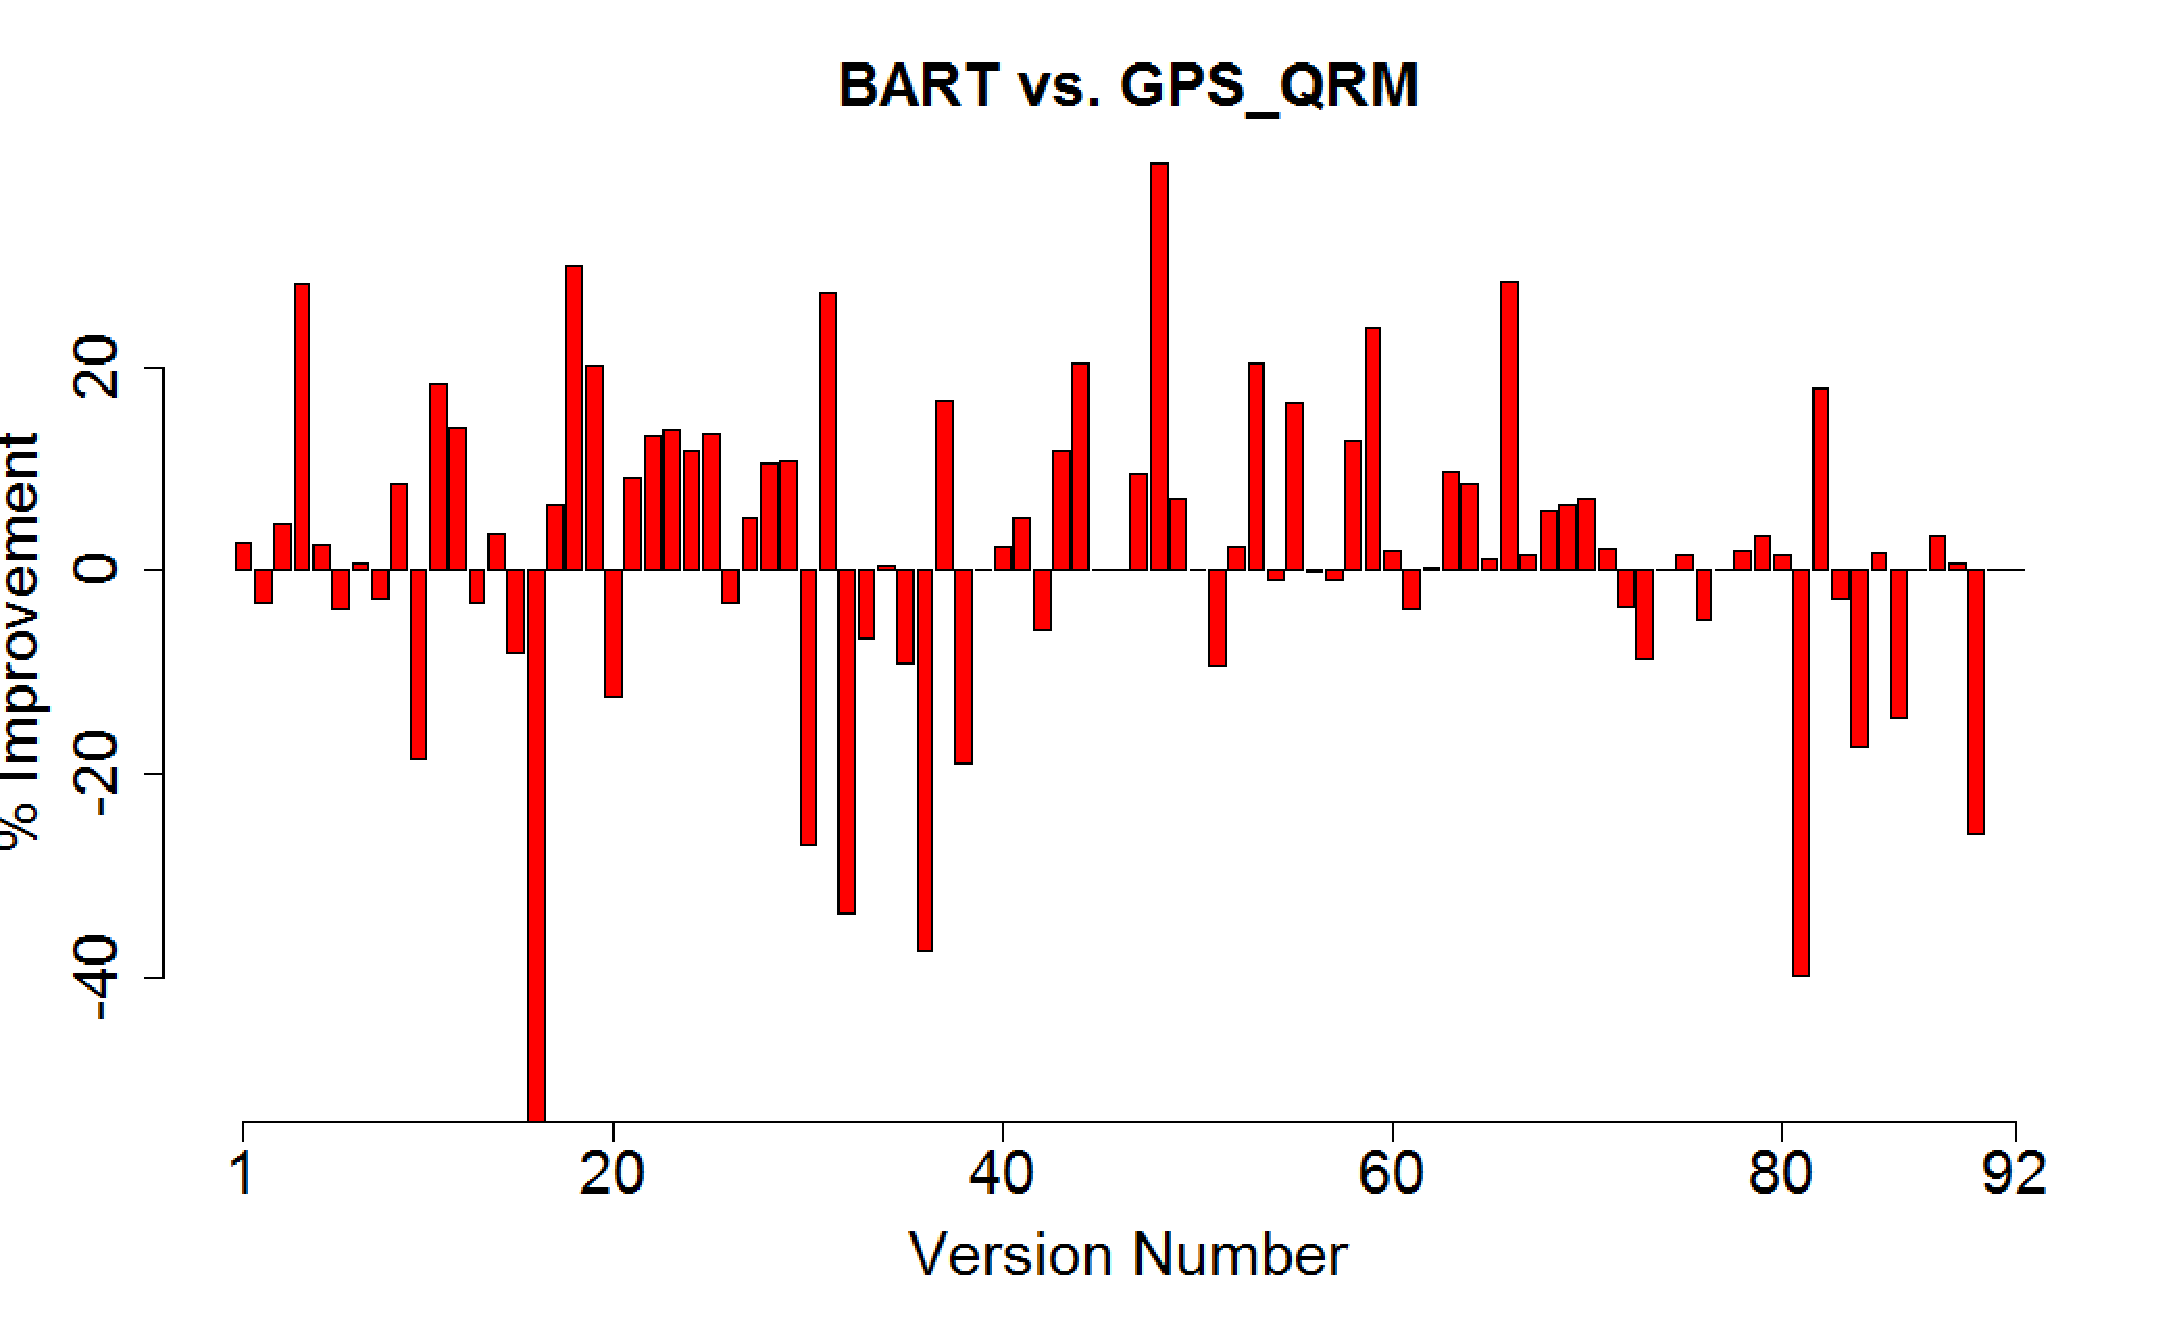
\includegraphics[width=0.8\textwidth]{chapter4_BARTvsGPS_QRM.pdf}
\caption{Relative performance of NUMFL-GPS-QRM with and without data from passing runs, on individual single-fault program versions.}
\label{BARTvsQRM}
\end{figure*}

\begin{figure*}[!thpb]
\centering
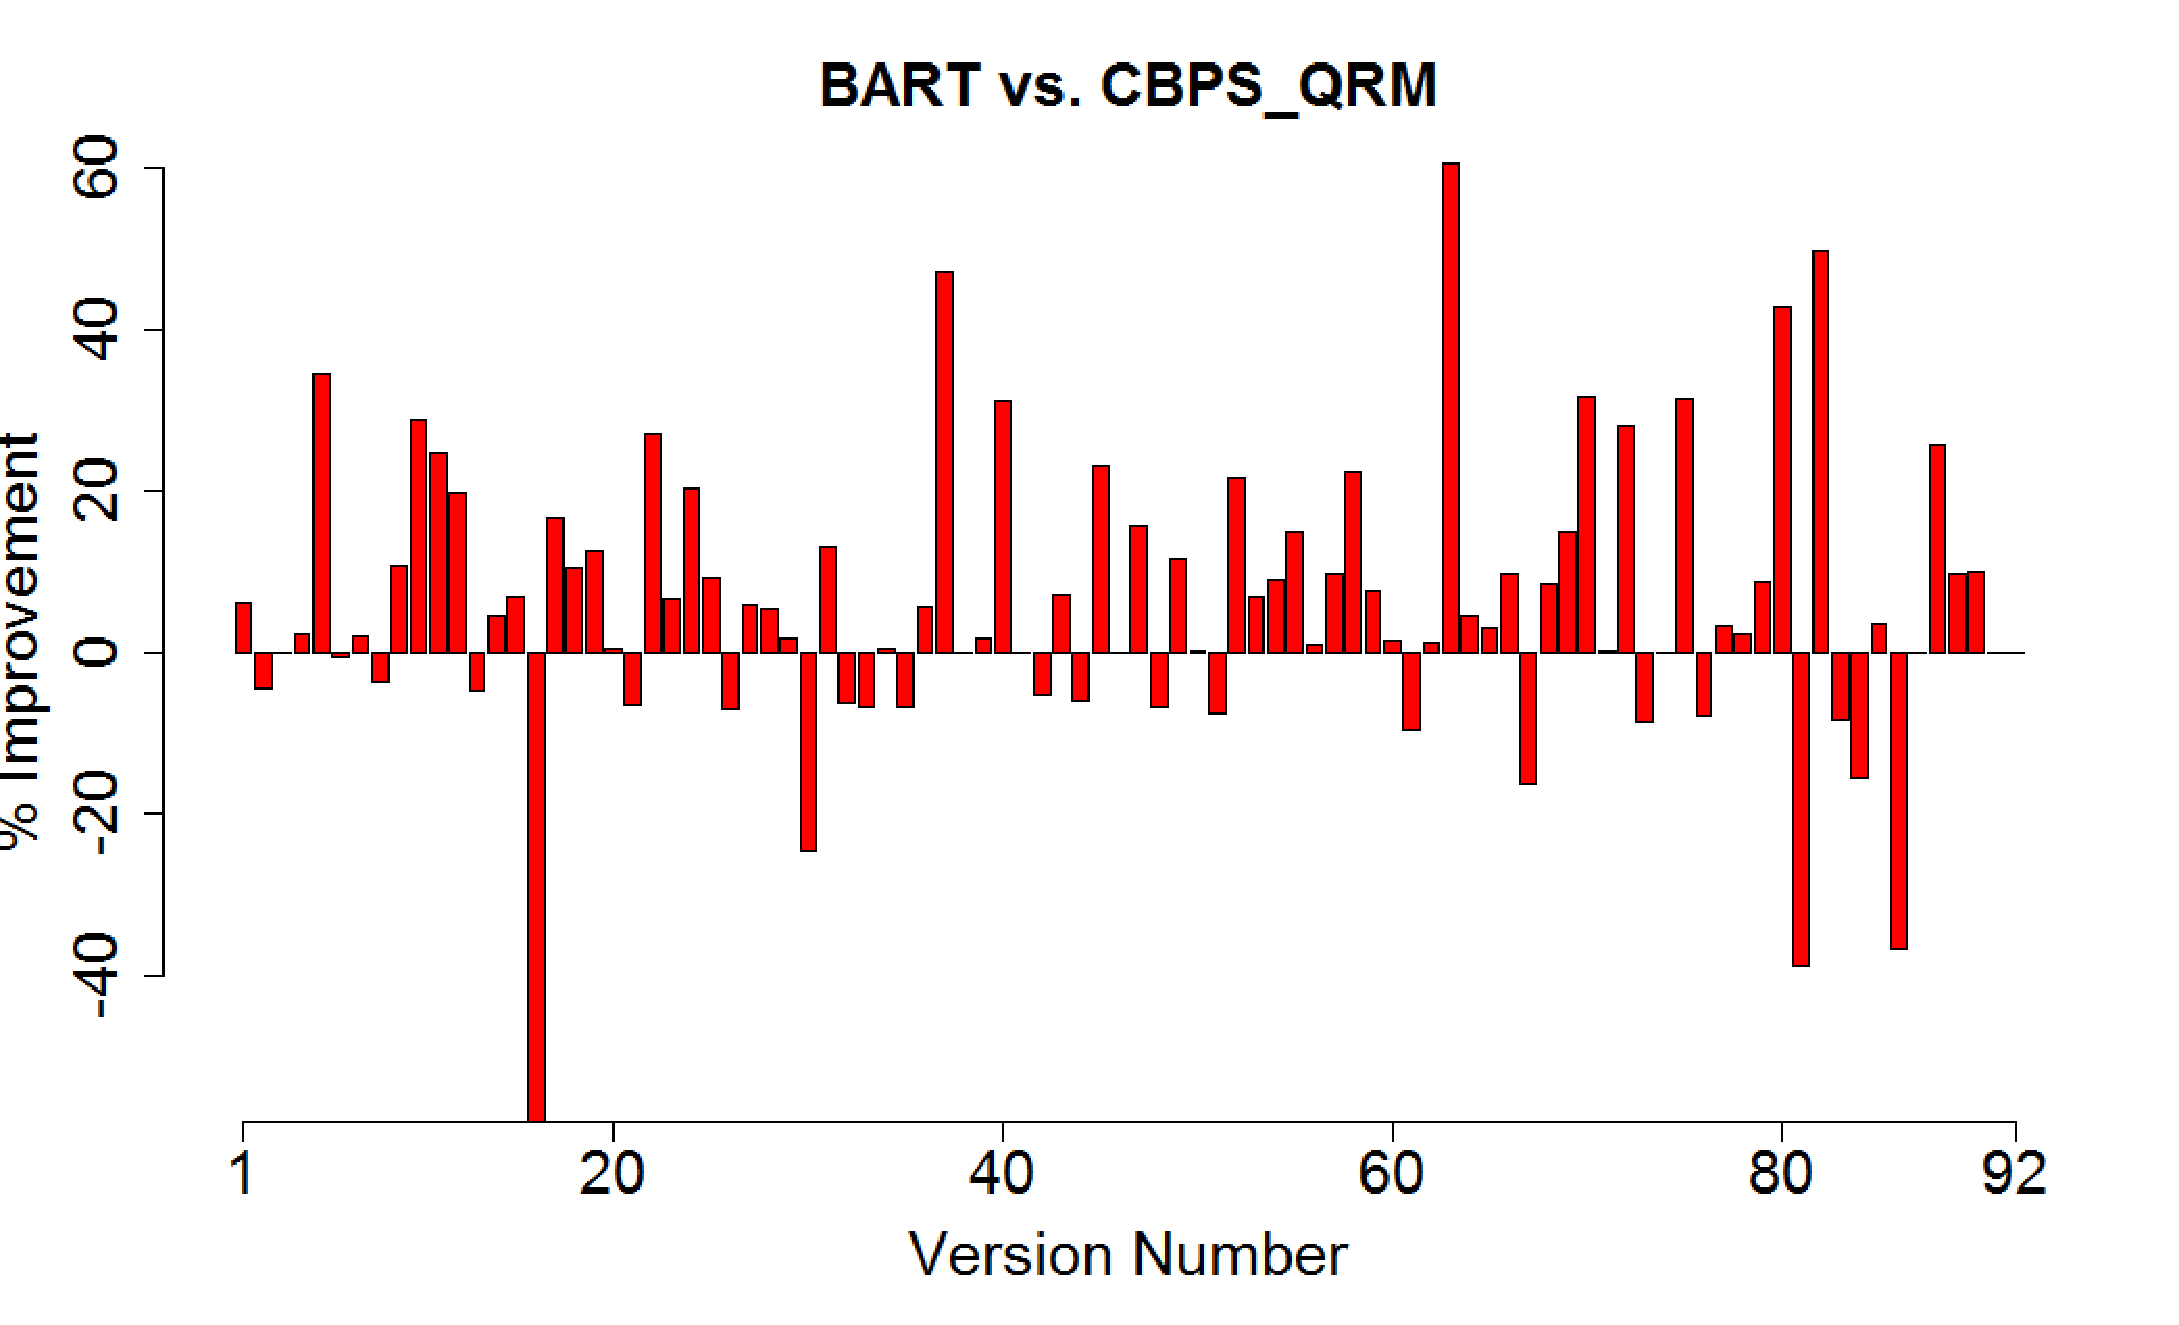
\includegraphics[width=0.8\textwidth]{chapter4_BARTvsCBPS.pdf}
\caption{Relative performance of NUMFL-GPS-QRM with and without data from passing runs, on individual single-fault program versions.}
\label{BARTvsCBPS}
\end{figure*}

Table \ref{tableBARTvsNUMFL_M} shows the average cost, over the faulty versions of each subject program into which two faults were injected, of localizing the first fault to be found, for both BART and NUMFL.  From Table \ref{tableBARTvsNUMFL_M}, the average cost of BART is close to that of NUMFL-GPS-QRM on two faults subject programs. BART performed better than NUMFL-GPS-QRM on the versions of  2 subject programs, but performed worse than NUMFL-GPS-QRM on the versions of 3 subject program.  BART performed better than NUMFL-CBPS-QRM on the versions of 4 subject programs, but performed worse than NUMFL-CBPS-QRM on the versions of only 1 subject program.

Figure \ref{BARTvsGPS_M} graphically contrasts the performance of the BART and NUMFL-GPS-QRM on the individual two-fault versions.  BART performed better than NUMFL-CBPS-QRM on 13 versions and NUMFL-GPS-QRM performed worse on 12 versions.  BART performed at least 10\% better than NUMFL-GPS-QRM on 7 versions, whereas NUMFL-CBPS-QRM performed at least 10\% better than NUMFL-GPS-QRM on just 1 version. Figure \ref{BARTvsCBPS_M} graphically contrasts the performance of the BART and NUMFL-CBPS-QRM on the individual two-fault versions.  BART performed better than NUMFL-CBPS-QRM on 13 versions and NUMFL-CBPS-QRM performed worse on 12 versions.  BART performed at least 10\% better than NUMFL-CBPS-QRM on 7 versions, whereas NUMFL-CBPS-QRM performed at least 10\% better than NUMFL-GPS-QRM on just 1 version.

\begin{table*}[htbp!]
\caption{AVERAGE FAULT LOCALIZATION COSTS OF BART AND NUMFL ON MULTIPLE-FAULT PROGRAM VERSIONS}
\label{tableBARTvsNUMFL_M}
\centering
      \begin{tabular}{|l|c|c|c|}
      \hline
\multirow{2}{*}{Subject Program}	& \multirow{2}{*}{BART}&	\multicolumn{2}{|c|}{{\bf NUMFL}}	\\	\cline{3-4}
& & GPS-QRM	&CBPS-QRM \\ \hline
Apache\_EigenDecompose	&7.98	\%&10.3\%	&	11.1\%	\\	\hline
Apache\_DScompiler	&	5.13\%&4.5\%	&	5.9\%	\\	\hline
Apache\_Rotation3D	&	10.69\%&7.0\%	&	3.0\%	\\	\hline
Ojaljo\_SchurDecompose	&17.55	\%&5.4\%	&	19.8\%	\\	\hline
Jama\_MatrixDecompose	&	4.65\%&14.1\%	&	23.4\%	\\	\hline
{\bf Average Cost} &9.20\% &8.26\% &12.64\%\\ \hline
\end{tabular}
\end{table*}

\begin{figure*}[!thpb]
\centering
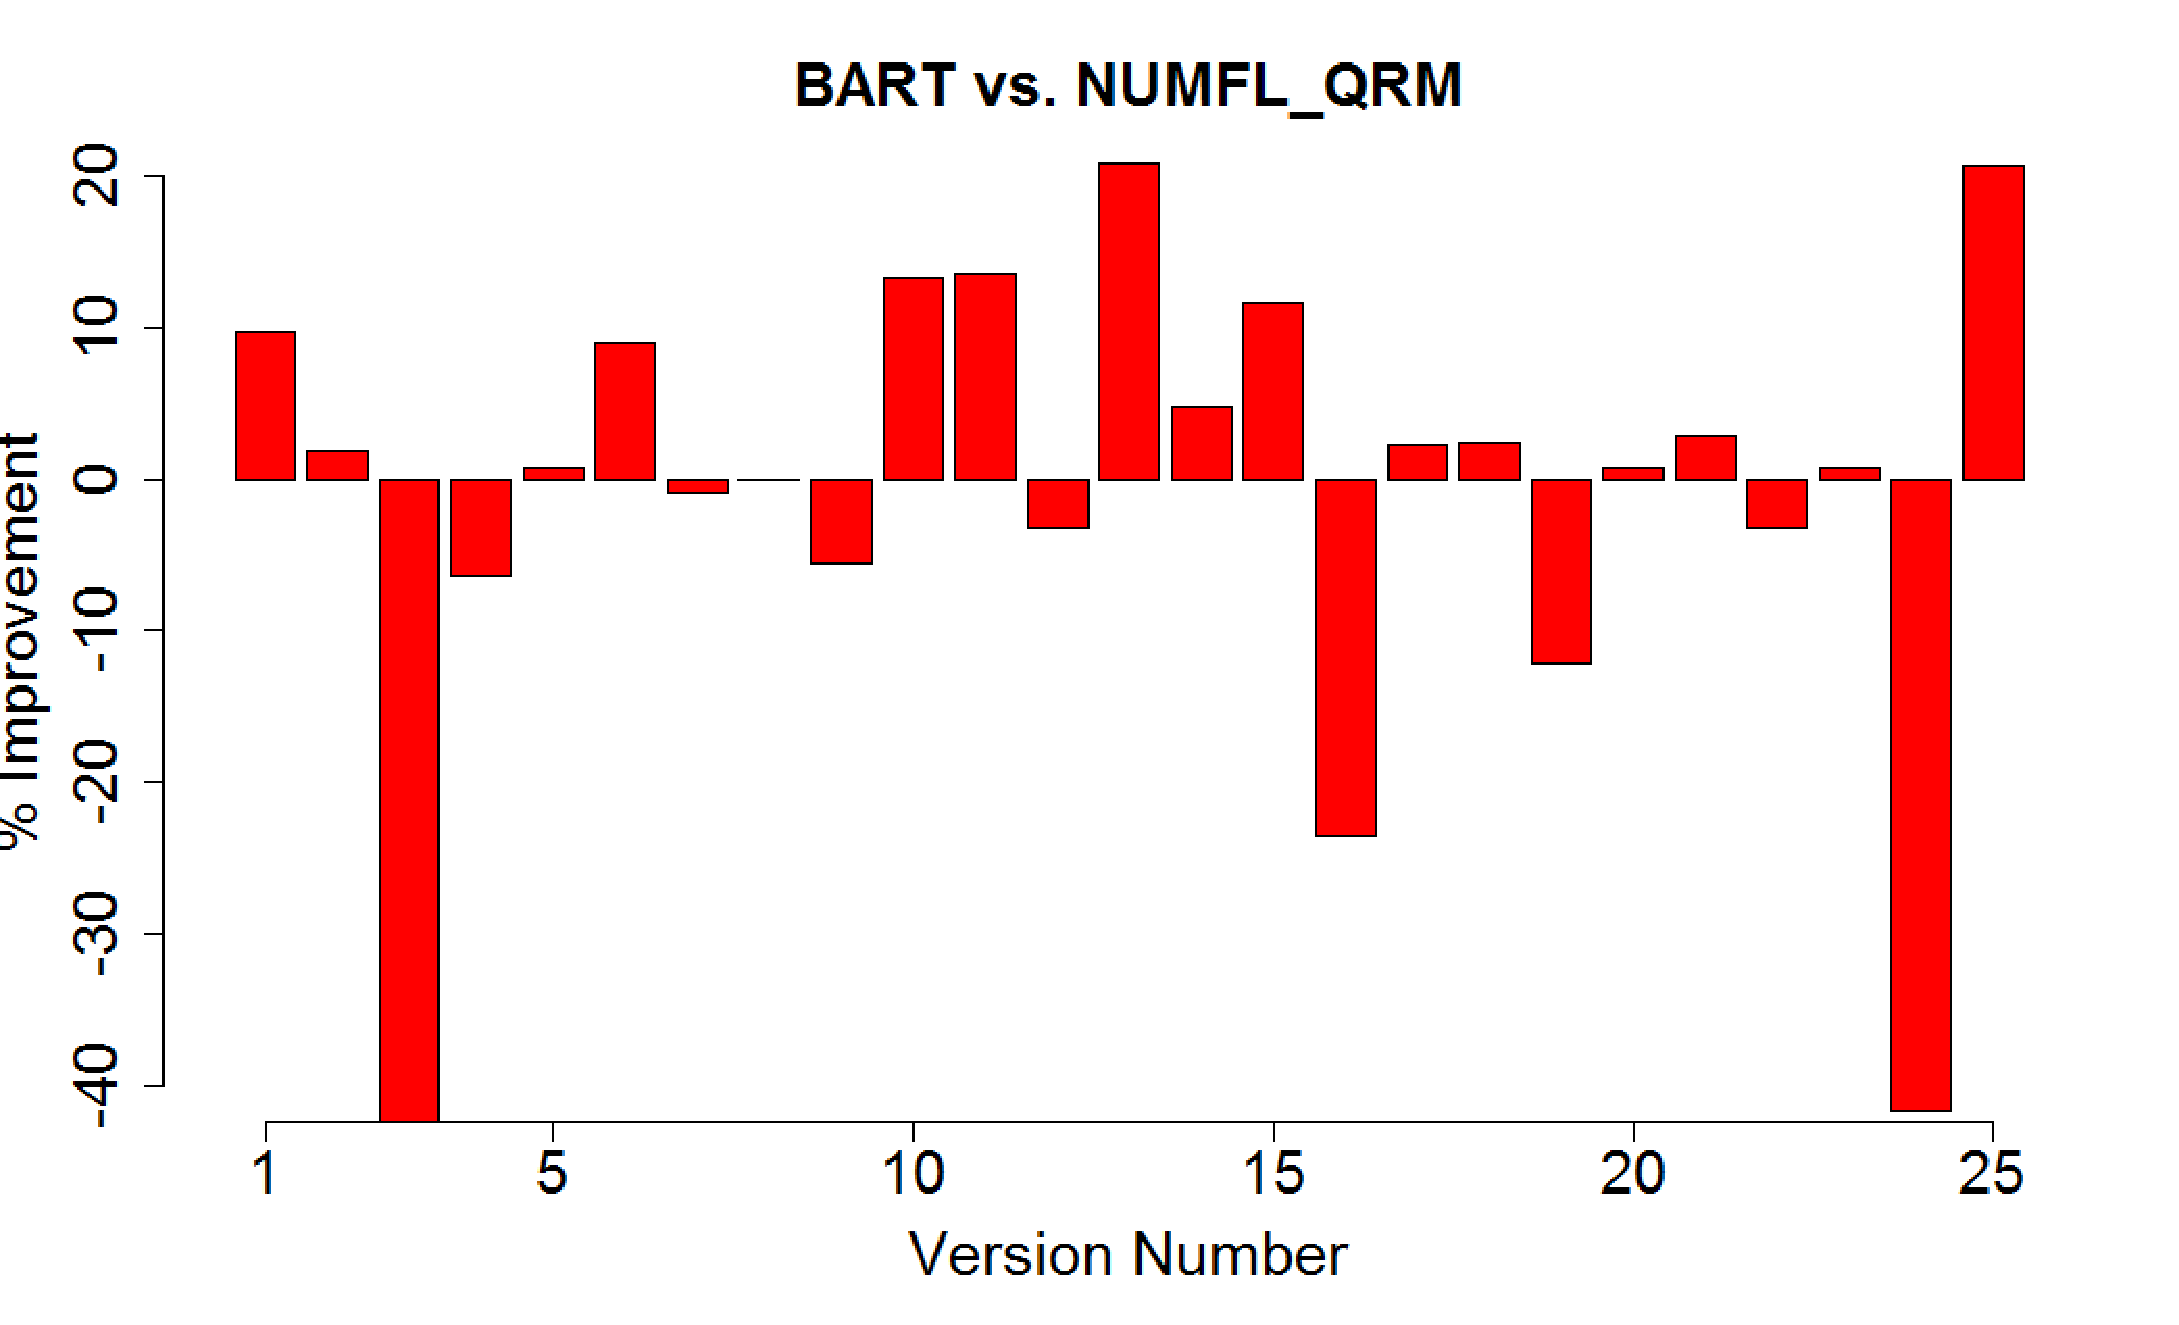
\includegraphics[width=0.8\textwidth]{chapter4_BARTvsGPS_QRM_M.pdf}
\caption{Relative performance of NUMFL-GPS-QRM with and without data from passing runs, on individual single-fault program versions.}
\label{BARTvsGPS_M}
\end{figure*}

\begin{figure*}[!thpb]
\centering
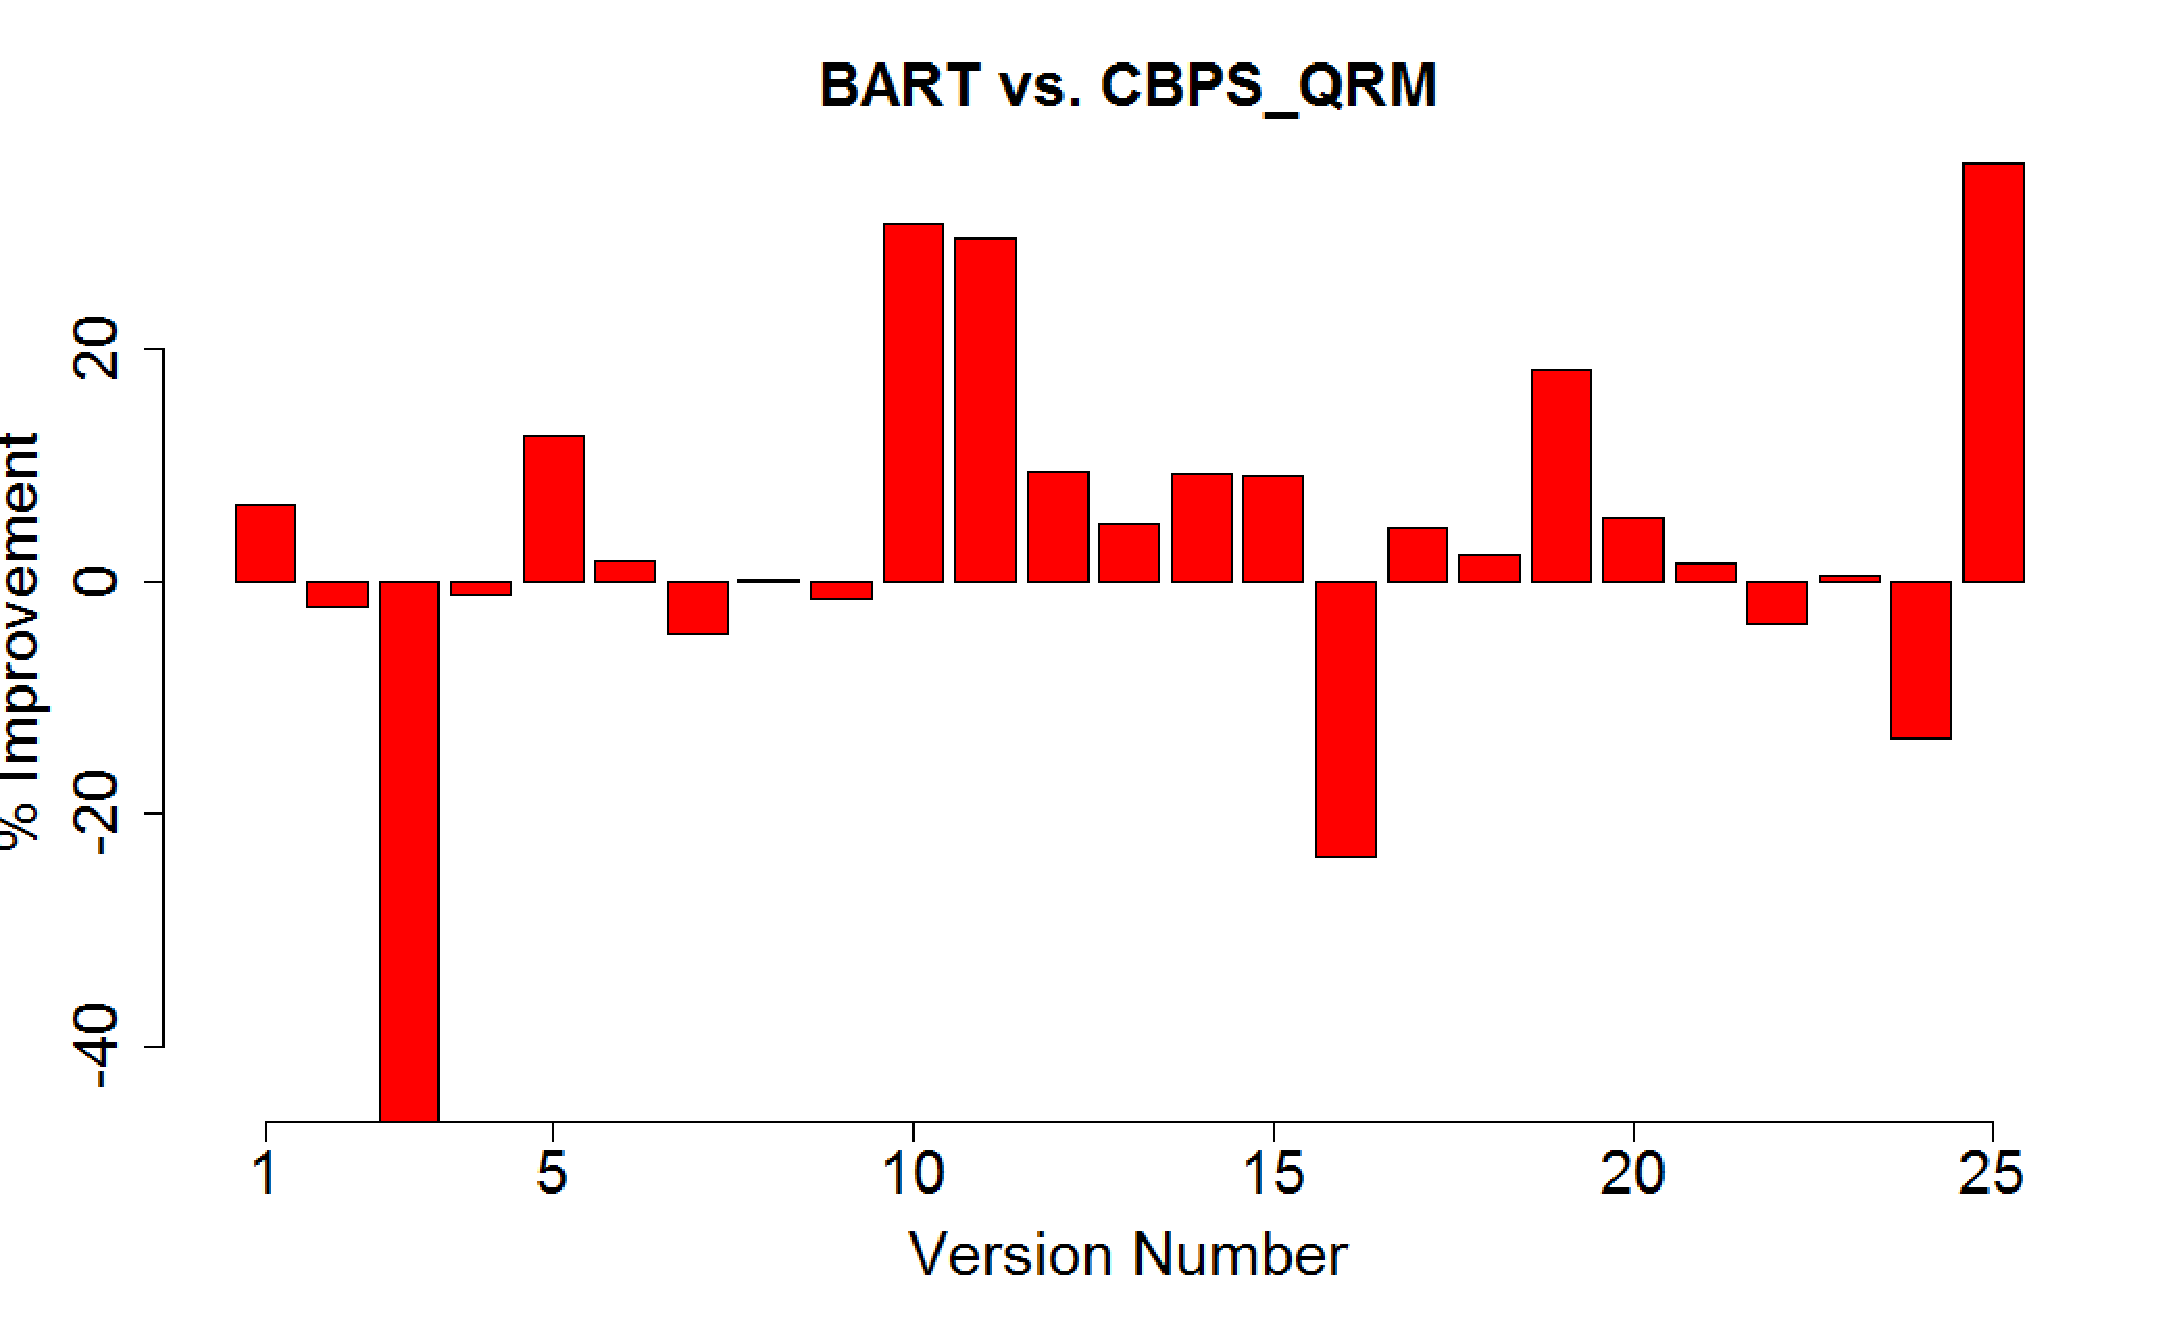
\includegraphics[width=0.8\textwidth]{chapter4_BARTvsCBPS_M.pdf}
\caption{Relative performance of NUMFL-GPS-QRM with and without data from passing runs, on individual single-fault program versions.}
\label{BARTvsCBPS_M}
\end{figure*}

\subsection{Sensitivity of BART model on the number of trees and number of tests}\label{BARTsensitivity}

In previous sections, we use the full observational data of tests to fit a BART model with 10 trees in the sum of trees structure. In this section, we will analyze if increasing number of trees or decreasing the number of tests would influence the performance of BART. In Table \ref{sensitivity}, the first column of numbers is the fault localization cost of BART model contains 10 trees and fitted with full observational data (3000-8000 tests). The second column of numbers is the fault localization cost of BART model contains 50 trees and fitted with full observational data. The third column of numbers is the fault localization cost of BART model contains 10 trees but fitted with only 300 tests' data. From Table \ref{sensitivity}, when increased the number of trees from 10 to 50, BART model has better performance on 6 subject programs. But there are also 6 subject program where BART model's performance become worse after increasing the number of trees. The average cost across 16 subject programs is roughly same: 10.52\% for BART model with 10 trees and 10.58\% for BART model with 50 trees. This means 10 trees are enough to handle the nonlinearity problem in AFCE estimation.  When decrease the number of tests to 300, the average cost is slightly increased to 10.74\%.  This means BART model does not require a large number of tests to localize bugs in numerical software.

\begin{table*}[htbp!]
\caption{AVERAGE FAULT LOCALIZATION COSTS OF BART MODEL WITH DIFFERENT NUMBER OF TREES AND TESTS ON ONE SINGLE-FAULT PROGRAM VERSIONS }
\label{sensitivity}
\centering
      \begin{tabular}{|l|c|c|c|}
      \hline
\multirow{2}{*}{{\bf Subject Program}}	&	\multicolumn{3}{|c|}{{\bf BART Model}}	\\	\cline{2-4}
& 10 trees & 50 trees & 300 tests\\ \hline
Apache\_EigenDecompose			&	2.50	\%	&	3.07	\%	&	2.38	\%	\\ \hline
Apache\_DScompiler			&	9.72	\%	&	8.61	\%	&	9.64	\%	\\ \hline
Apache\_BigMatrix			&	9.00	\%	&	9.05	\%	&	9.00	\%	\\ \hline
Apache\_Rotation3D			&	9.07	\%	&	8.73	\%	&	8.16	\%	\\ \hline
Ojaljo\_SchurDecompose			&	10.61	\%	&	9.89	\%	&	11.44	\%	\\ \hline
Jama\_MatrixDecompose			&	11.62	\%	&	11.16	\%	&	11.32	\%	\\ \hline
SciMark\_LU			&	8.33 \%	&	9.72	\%	&	6.94	\%	\\ \hline
SciMart\_FFT			&	27.59	\%	&	26.72	\%	&	27.59	\%	\\ \hline
Apache\_SymmLQ			&	1.75	\%	&	1.75	\%	&	1.75	\%	\\ \hline
Apache\_SplineInterpolator			&	37.78	\%	&	40	\%	&	45.56	\%	\\ \hline
Apche\_SimpleRegress			&	1.70	\%	&	1.70	\%	&	1.70	\%	\\ \hline
Apache\_SchurTransformer			&	4.56	\%	&	4.88	\%	&	4.23	\%	\\ \hline
Apache\_MillerUpdatRegress			&	1.24	\%	&	1.24	\%	&	1.24	\%	\\ \hline
Apache\_HarmonicFitter			&	30.10	\%	&	30.08	\%	&	28.06	\%	\\ \hline
Apache\_FastSine			&	1.53	\%	&	1.53	\%	&	1.53	\%	\\ \hline
Apache\_FastCosine			&	1.29	\%	&	1.29	\%	&	1.29	\%	\\ \hline
Average Cost 	&	10.52\% 	&10.58\% 	&10.74\%	\\ \hline
\end{tabular}
\end{table*}

\subsection{Computation Time Analysis}
In this study, we use a Dell Precision T5600 with two 2.30 GHz intel Xeon CPUs and 64 GB RAM. Table \ref{BARTcomputetime} summarized the average computation time of the three BART models described in last section on each subject program.  When the number of trees increased from 10 to 50, the average computation cost nearly doubled. If we reduced number the tests from more than 3000 to 300, the computation cost will reduced more than 50\%.  From Table \ref{BARTcomputetime} and Table \ref{sensitivity}, we can conclude that the BART model with 10 trees and fitted with 300 tests get the best cost-performance ratio among the three BART models fitted with different settings. But we also need to point out that even the BART model is fitted with 300 tests, its computation cost is still about twice of the computation cost of NUMFL. Thus, the computation cost is a weakness of applying BART model on localizing faults in numerical programs. 

\begin{table*}[htbp!]
\caption{AVERAGE COMPUTATION TIME OF NUMFL-GPS-QRM AND NUMFL-CBPS-QRM ON ONE SINGLE-FAULT PROGRAM VERSIONS }
\label{BARTcomputetime}
\centering
      \begin{tabular}{|l|c|c|c|}
      \hline
\multirow{2}{*}{{\bf Subject Program}}	&	\multicolumn{3}{|c|}{Average Computation Time (Secs)}	\\	\cline{2-4}
& 10 trees & 50 trees & 300 tests\\ \hline

Apache\_EigenDecompose	&	2856.73	&	5530.20	&	1205.97	\\ \hline
Apache\_DScompiler	&	628.31	&	1243.78	&	274.88	\\ \hline
Apache\_BigMatrix	&	696.58	&	1337.73	&	292.28	\\ \hline
Apache\_Rotation3D	&	2668.41	&	5550.45	&	1082.64	\\ \hline
Ojaljo\_SchurDecompose	&	2636.96	&	5013.37	&	1313.53	\\ \hline
Jama\_MatrixDecompose	&	3134.49	&	6005.71	&	1262.88	\\ \hline
SciMark\_LU	&	167.94	&	332.45	&	121.38	\\ \hline
SciMart\_FFT	&	393.26	&	842.31	&	234.09	\\ \hline
Apache\_SymmLQ	&	908.12	&	1986.32	&	245.21	\\ \hline
Apache\_SplineInterpolator	&	364.80	&	747.42	&	135.00	\\ \hline
Apche\_SimpleRegress	&	823.34	&	1685.88	&	227.27	\\ \hline
Apache\_SchurTransformer	&	768.44	&	1539.44	&	315.65	\\ \hline
Apache\_MillerUpdatRegress	&	396.10	&	808.59	&	198.61	\\ \hline
Apache\_HarmonicFitter	&	326.09	&	673.73	&	120.28	\\ \hline
Apache\_FastSine	&	1006.86	&	2064.98	&	259.78	\\ \hline
Apache\_FastCosine	&	1089.13	&	2229.39	&	294.56	\\ \hline
\end{tabular}
\end{table*}

\section{RELATED WORK}\label{BARTrelatedwork}
The most related works to this study are those using BART model to estimate treatment causal effect. Hill et al. proposed to apply BART model for causal inference and data science \cite{hill2012bayesian, hill2013assessing}. In the paper, they designed the method of using BART to estimate average causal effect of binary treatment variable and discussed how to use BART to handle continuous treatment variables and outcome missing data. Later, Green et al. applied BART to model heterogeneous treatment effects \cite{green2012modeling}. Sparapani et al. extends the usefulness of BART in medical applications by addressing needs arising in survival analysis \cite{sparapani2016nonparametric}.

Another related work is using tree structure in fault localization. Chen et al \cite{chen2004failure} present a decision tree learning approach to identify the causes of failures in internet sites. Francis et al \cite{francis2004tree} use tree based method to classify software failures. Kiciman et al \cite{kiciman2005root} use decision tree to diagnose which component of large scale systems is the root cause of failure. However, unlike our models, all their works do not localize the fault on statement level.

\section{CONCLUSION}\label{BARTconclusion}
BART model is a Bayesian non-parametric model which can capture both nonlinearities and interactions between variables without knowing the information about how these variables are parametrically related . BART uses a sum of trees structure to approximate the dose response function of continuous treatment variables. The AFCE can be estimated by averaging the causal effect of treatment on outcome at each observation unit. We reported the result of an empirical comparison of BART model to several competing fault localization metrics on both single-fault subject programs and multiple-fault subject programs. BART model performed significantly better than the other techniques. We also compare the BART model with NUMFL, which is introduced in chapter 3. The result shows BART model outperforms NUMFL on single faults localization. In multiple faults localization, BART and NUMFL has similar performances.  We also study the sensitivity of the BART model to the number of trees and the number of tests. The result shows BART is robust on the sample size and number of trees.   
%\chapter{Studying disease comorbidity network to detect genetic evidences for disease links: application on colorectal cancer and obesity}\label{cancer}

\section{Motivation}

A number of epidemiological studies suggest that
obesity increases the risk of colorectal cancer (CRC)
\cite{calle2003overweight,bardou2013obesity,khaodhiar1999obesity}.
Based on these evidences of co-occurrence,
many genetic factors have been proposed to explain the role of obesity in the development of CRC.
For example, both animal and human studies have demonstrated that the
increased release of insulin and reduced insulin signaling play roles
in obesity and colorectal carcinogenesis \cite{pollak2008insulin,leroith2003insulin,renehan2004insulin}.
Experiments also show that obesity leads to altered level of adipocytokines,
such as Adiponectin \cite{dalamaga2012role,an2012adiponectin,wei2005low}
and leptin \cite{stattin2003plasma,tamakoshi2004leptin}, which may either prevent or foster carcinogenesis.

The mechanism for the association between obesity and CRC is multifactorial and inconclusive
\cite{khaodhiar1999obesity,danese2012role}. Shared comorbidities between
obesity and CRC can provide unique insights into the common genetic basis for the two diseases.
For example, type 2 diabetes is highly correlated with obesity and was identified as a risk factor
for CRC \cite{berster2008type}. A few studies then discovered that genetic factors
of insulin resistance, which occur in type 2 diabetes, contribute in explaining the role of obesity
in CRC \cite{komninou2003insulin}. However, both obesity and CRC are heterogeneous conditions.
Over 40\% of the obese population is not characterized by the presence of insulin
resistance \cite{mesquita2009metabolically}. We hypothesize that systems approaches
to studying the diseases that are phenotypically-significant to
both CRC and obesity may offer new insights into the
common molecular mechanisms between the two interconnected diseases.

Systematic comorbidity studies have been conducted previously,
but mostly focused on pairwise comorbidities and their genetic overlaps.
Rhetsky et al. developed a statistical model to estimate the co-occurrence
relationship for each pair of 160 diseases \cite{rzhetsky2007probing},
and demonstrated that comorbidities are genetically linked. Park et al. \cite{park2009impact}
and Hidalgo et al. \cite{hidalgo2009dynamic}
detected the comorbidities pairs from the Medicare claims
(which only contain senior patients ages 65 or older) with statistical measures.
Roque et al. mined pairwise disease correlations using similar measures from
medical records of a psychiatric hospital \cite{roque2011using}.


In this study, we developed a novel approach to detect diseases
that have strong connections with both obesity and CRC in a comorbidity network.
Specifically, we first mined disease comorbidity relationships from a new data source and constructed
a novel disease comorbidity network. Then we extracted the local network consisting of all the
paths between obesity and CRC, and prioritized the nodes (diseases) that play critical roles
in maintaining the connection between the two diseases (Fig.\ref{crchypothesis}). Substantial literature evidences can support that the top ranked diseases have associations with both obesity and CRC. We investigated the gene expression profiles of a prioritized comorbid disease to facilitate detecting novel genetic basis underlying the link between obesity and CRC. Our approach is generalizable to study the genetic basis for other disease associations.
\begin{figure}[!tpb]
\vspace{-.1cm}
\centerline{\includegraphics[width=0.5\textwidth]{Chap5_crc_hypothesis.eps}}
%\vspace{-5cm}
\caption{Approach to detect the diseases that have strong connections with both obesity and CRC in the comorbidity network. Nodes D1, D2 and D3 were prioritized because they play important roles in maintaining the network structure and the connection. }
\vspace{-0cm}
\label{crchypothesis}
\end{figure}

\section{Data and methods}
Fig.\ref{crcmethod} shows the steps of our approach.
We first mined disease comorbidity relationships from large amounts of patient records
in a public database and constructed a disease comorbidity network.
We then extracted the local comorbidity cluster for obesity and CRC
and prioritize the candidate comorbidity that plays a critical role in connecting the two diseases.
Finally we conducted gene expression meta-analysis to
identify common genes shared by obesity, CRC and the prioritized comorbidity.
\begin{figure}[!tpb]
\vspace{-.1cm}
\centerline{\includegraphics[width=1\textwidth]{Chap5_crc_method.eps}}
%\vspace{-5cm}
\caption{Our approach contains three steps: (1) We constructed a comorbidity network based on data mining; (2) we extracted the local network that contains paths from obesity to CRC, and analyzed the local network to pin point the strong comorbidity for both obesity and CRC; (3) we conducted gene expression meta-analysis to identify common genes shared among obesity, CRC and the comorbidity. }
\vspace{-0cm}
\label{crcmethod}
\end{figure}

\subsection{Construct disease comorbidity network}
\subsubsection{Data sets for comorbidity mining}
The adverse event reports contain records of 3,354,043 patients.
Among all patients, 66\% and 94\% have their age and gender information available.
Figure \ref{distr}(a)-(b) show distributions of age and gender.
Unlike the Medicare system, FAERS contains patients in of ages
from one day to hundreds of years.
The distributions are not severely inclined to particular gender or age levels.
\begin{figure}[!ht]
\vspace{-0.6cm}
\begin{center}
\includegraphics[width=\textwidth]{Chap5_demographics.eps}
\end{center}
\vspace{-0.5cm}
\caption{
{(a) Age distribution of the patients in the adverse event reports. (b) Gender distribution. (c) Distribution of disease semantic types: T047, Disease or Syndrome; T020, Acquired Abnormality; T046, Pathologic Function; T184, Sign or Symptom; T033, Finding; T190, Anatomical Abnormality; T191, Neoplastic Process; T048, Mental or Behavioral Dysfunction; T049, Cell or Molecular Dysfunction; T019, Congenital Abnormality; T037, Injury or Poisoning.}
}
\vspace{-0.5cm}
\label{distr}
\end{figure}

The data represents the diseases that patients have by 10,122 indications of drugs that patients take.
These indication terms include not only diseases, but also treatment procedures, such as surgery; common symptoms, such as pain; and ill-defined events, such as unevaluable events.
We mapped the indication terms to the concept unique identifiers (CUIs)
in Unified Medical Language System (UMLS) and extracted their semantic types.
Figure \ref{distr}(c) listed the distribution of eleven semantic types, in which
the types such as ``disease or syndromes," ``neoplastic process," and ``mental or behavioral dysfunction"
contain disorder concepts.
With the disease data for million of patients, we were able to conduct large-scale comorbidity mining and extract
interesting disease associations.

\subsubsection{Preprocess data}
We developed an automatic pipeline to preprocess the patient-indication pairs (Figure \ref{dataworkflow}).
We mapped all indication terms to CUIs and classified them by semantic types using the UMLS metathesaurus.
Then We selected the identifiers of six semantic types: Mental or Behavioral Dysfunction, Neoplastic Process, Acquired Abnormality, Congenital Abnormality, Disease or Syndrome, and Anatomical Abnormality. We combined the synonyms among terms corresponding to these identifier and removed those only appearing once in the data, since rare diseases may lead to unstable association patterns. Finally, the data contains 3,033,368 links between 2,371,406 patients and 3,994 diseases.
\begin{figure}[!ht]
%\vspace{-0.6cm}
\begin{center}
\includegraphics[width=\textwidth]{Chap5_dataworkflow.eps}
\end{center}
\vspace{-0.5cm}
\caption{
{Automatic pipeline to pre-process the patient-disease data in adverse event reports and mine comorbidity patterns}
}
\vspace{-0.5cm}
\label{dataworkflow}
\end{figure}


\subsubsection{Mine comorbidity patterns}
We explored comorbidity patterns among the 3,994 diseases with association rule mining.
Due to the large number of patients and diseases in the adverse event reports,
exhausting all possible association patterns is computationally impractical.
We applied the frequent pattern growth algorithm,
which uses an tree structure to compress the input and grow
the patterns in a bottom-up manner \cite{han2000mining}.
Previous effort has demonstrated that this algorithm outperforms other popular pattern mining methods,
such as the Apriori algorithm \cite{agrawal1994fast}.
The frequent pattern growth algorithm has also been successfully
applied in biomedical domain to extract drug adverse effects \cite{luo2013mining}.
Association rule mining can flexibly detect strong co-occurrence relationships among sets of diseases, and alleviates the intrinsic bias of traditional comorbidity measures (such as relative risk and $\phi$-correlation) towards rare diseases.

We implemented the algorithm using the Weka java package \cite{hall2009weka}.
The result of the algorithm is a set of patterns indicating how diseases are associated with each other.
The pattern between two sets of diseases is
represented in the form ${\rm{X}} \Rightarrow {\rm{Y}}$,
where $X$ is the pattern body and $Y$ is the pattern head.
For example, $[anxiety, amnesia] \Rightarrow [depression]$
indicates that when patients have anxiety and amnesia,
are also likely to have depression.
Note that though each pattern is directed with an arrow,
they do not indicate causations between diseases,
but represent co-occurrences. To avoid confusion,
we currently ignored the directions of patterns,
 considered all diseases in set $X$ and $Y$ associated.

The mining algorithm requires a few parameters:
the minimum support was set to 0.0008\%, which means
at least 20 patients should have all the diseases
in each pattern at the same time; the maximum
number of diseases in each pattern was set at 3;
and confidence was chosen to measure and rank the patterns.
The confidence score of pattern ${\rm{X}} \Rightarrow {\rm{Y}}$ is defined as:
\begin{equation}
confidence(X \to Y) = |X \cup Y|/|X|\label{arm},
\end{equation}
where $|X \cup Y|$ is the number of patients who have diseases
in both $X$ and $Y$, and $|X|$ is the number of patients who have diseases in $X$.

\subsubsection{Construct disease comorbidity network }
We constructed an undirected and unweighted comorbidity network
based on the result of association rule mining,
which is a list of patterns between two sets of diseases,
represented in the form $x \to y$.
We collected all diseases in the set x and y in each pattern, a
ssuming they have comorbidity relationships with each other,
and established an edge between each pair of diseases in $x \cup y$ to construct the comorbidity network.

\subsection{Prioritize the diseases that have strong associations with both obesity and CRC}
We extracted the local network consisting of  the paths from obesity to CRC in the disease comorbidity network. The local network thus includes the nodes that may represent different aspects of the relationship between obesity and CRC. We implemented breath first search to enumerate the paths, and limited the paths within four steps.
Then we ranked the nodes in the local network, except obesity and CRC, based on how important they are in maintaining the local network structure and the connection between obesity and CRC. We used the degree and betweenness centrality to characterize the importance of each node in the flowing of the network. The degree of a node becomes higher if more paths between obesity and CRC pass through this node. The betweeness evaluates the number of times that the node acts as the bridge along the shortest paths. Removing the nodes with highest degree or betweenness can easily break down the connection between obesity and CRC. We investigated the top ranked diseases based on both ranking methods, and used the unexpected ones to guide the detection of genetic associations between obesity and CRC.

\subsection{Identify gene overlaps through gene expression meta-analysis}
We chose a top ranked disease on the path between obesity and CRC, and then conducted gene expression meta-analysis for the prioritized disease, obesity and CRC, respectively, to detect new genetic explanations for the relationship between obesity and CRC. Gene expression normalized data (SOFT files) were downloaded from NCBI GEO omnibus (GEO, http://www.ncbi.nlm.nih.gov/geo/) using the R package GEOquery \cite{davis2007geoquery}. Then, we performed microarray meta-analyses for each disease independently using the R package MetaDE \cite{wang2012r}. MetaDE implements meta-analysis methods for differential expression analysis, and we used the Fisher's method. Significant differentially expressed genes (DEGs) were selected as those displaying a FDR corrected p-value <0.05. Last, we extracted the common significant genes for the three diseases.

\section{Results}
\subsection{Local disease comorbidity network models the connection between obesity and CRC}
We extracted 7006 comorbidity association rules with the confidence larger than 50\% from the patient records across ten years. The comorbidity network based on these  rules contains 771 nodes and 15,667 edges. Fig.\ref{localnet} shows the local network consisting of all the 119 paths (no longer than four steps) from obesity to CRC. A total of 24 nodes in the local network are the candidate diseases, which have associations with both obesity and CRC, and may indicate different aspects of the relationship between the two diseases.

\subsection{Osteoporosis shows high comorbidity associations with both CRC and obesity}
Table \ref{noderank} shows the top five nodes sorted by degree and betweenness in the local network. In either way of ranking, hypertension, diabetes and hyperlipaemia were in top three and closely related with both obesity and CRC. Substantial literature evidences support that the metabolic syndrome components, hypertension and hyperlipaemia, as well as diabetes have association with obesity and CRC through insulin resistance in substantial literature \cite{khaodhiar1999obesity,pollak2008insulin,leroith2003insulin,renehan2004insulin,komninou2003insulin}. These three disorders also independently increase the risk of CRC and colorectal adenoma \cite{khaodhiar1999obesity,berster2008type,komninou2003insulin}.
The top ranked comorbidities demonstrated the validity of our network analysis approach.
\begin{figure}[!ht]
\vspace{-0.6cm}
\begin{center}
\includegraphics[width=6.5in]{Chap5_crc_localnet.eps}
\end{center}
\vspace{-0.5cm}
\caption{
{The local network that contains all paths from obesity to colorectal cancer in the comorbidity network.}
}
\vspace{-0.5cm}
\label{localnet}
\end{figure}

\begin{table}[h]
\caption{T\lowercase{OP FIVE DISEASE NODES IN THE LOCAL NETWORK THAT CONTAINS ALL PATHS FROM OBESITY TO COLORECTAL CANCER. THE DISEASES WERE RANKED BY DEGREE AND BETWEENNESS, RESPECTIVELY}.}
\label{noderank}
\centering
\begin{tabular}{ccccc}
\hline
\multirow{2}{*}{Rank} & \multicolumn{2}{l}{Ranked by degree} & \multicolumn{2}{l}{Ranked by betweenness} \\
                      & Nodes                  & Degree      & Nodes                  & Betweenness      \\\hline
1                     & Hypertension           & 26          & Hypertension           & 60.2             \\
2                     & Diabetes mellitus      & 24          & Diabetes mellitus      & 55.9             \\
3                     & Hyperlipaemia          & 22          & Hyperlipaemia          & 35.2             \\
4                     & Osteoporosis           & 14          & Osteoporosis           & 12.3             \\
5                     & Hypothyroid            & 14          & Hypothyroid            & 9.5 \\\hline
\end{tabular}
\end{table}

Significantly, osteoporosis was ranked highly by both centrality ranking methods. Epidemiological studies suggested an inverse association between bone mineral density and CRC \cite{nelson2002bone},
colon cancer among postmenopausal women \cite{ganry2008bone},
and colorectal adenoma \cite{nock2011higher}.
On the other hand, patients of obesity and osteoporosis may share common genetic and environmental factors \cite{zhao2007relationship}.
Different from previous studies, our result shows that osteoporosis is crucial for the association between CRC and obesity. Fig.\ref{localnet} shows the paths of obesity-osteoporosis-CRC. We further investigate the gene expression profiles of osteoporosis patients to gain novel insight of the genetic basis for the link between obesity and CRC.
\begin{figure}[!ht]
\vspace{-0.6cm}
\begin{center}
\includegraphics[width=0.7\textwidth]{Chap5_crc_osteo.eps}
\end{center}
\vspace{-0.5cm}
\caption{
{The paths from obesity to colorectal cancer that pass through osteoporosis.}
}
\vspace{-0.5cm}
\label{localnet}
\end{figure}

\subsection{Innovative genes shared among osteoporosis, obesity and CRC are detected using gene expression meta-analysis}

We downloaded five microarray series (GSE4017, GSE9348, GSE4183, GSE8671, GSE20916) for CRC, three (GSE48964, GSE29718, GSE55205) for obesity and three (GSE7429, GSE2208, GSE7158) for osteoporosis. Through meta-analysis, we obtained 9058 significant differentially expressed genes for CRC, 275 for obesity and 91 for osteoporosis. CRC and obesity shared a total of 192 genes. Among them, we found genes on insulin signaling pathways, such as PDK1, PRKAG2 and PDE3B, and adipocytokines, such as IL6 and IL8.

The three diseases osteoporosis, obesity and CRC shared six genes. Table \ref{genes} lists the genes and literature evidences, which support their relationships with each of the three diseases. Among them, FOS, JUN, and FOSB are oncogenes. FOS and JUN are known on the insulin signaling pathway. FOSB is on the AP1 pathway, which is associated with the proliferation of colon cancer cells \cite{ashida2005ap}.
Several studies suggested that overexpression of FOSB increases the responding of high fat reward while decreases energy expenditure and promotes adiposity \cite{thakali2014maternal,vialou2011role}.
\begin{sidewaystable}[h]
\caption{C\lowercase{OMMON GENES SHARED BY OBESITY, COLORECTAL CANCER AND OSTEOPOROSIS, AND PLAUSIBLE EVIDENCE SUPPORTING THEIR RELATIONSHIPS WITH THE THREE DISEASES}.}
\label{genes}
\centering
\begin{tabular}{l|m{4.5cm}|m{4.5cm}|m{4.5cm}}
GENES     & OBESITY                                                                                                                                                   & CRC                                                                                                 & OSTEOPOROSIS                                                                                                                        \\\hline
PPP1R15A* & In the bone morphogenetic protein (BMP) signaling pathway, which regulates appetite \cite{townsend2012bone}                                                              & Mutations in the BMP pathway are related with colorectal carcinogenesis \cite{hardwick2008bone}                 & In the bone morphogenetic protein signaling pathway, which are associated with bone-related diseases, such as osteoporosis \cite{chen2012tgf} \\
FOS       & diet-induced obesity is accompanied by alteration of FOS expression \cite{parker2013glucagon}                                                                    & Proto-oncogene, in the KEGG pathway of colorectal cancer \cite{kanehisa2000kegg}                                   & Mice lacking c-fos develop severe osteopetrosis \cite{okada1994mice}                                                                         \\
FOSB      & positive association between maternal obesity \cite{thakali2014maternal}                                                                                                   & Oncogene, regulators of cell proliferation, has a debatable impact on CRC patient survival \cite{pfannschmidt2009identification} & Overexpression of FosB increases bone formation \cite{sabatakos2000overexpression}                                                                           \\
HADHA*    & Associated with multiple fatty acid metabolism pathways \cite{liberzon2011molecular}                                                                                          & Unknown. Associated with breast cancer \cite{mamtani2012association}                                                    & Unknown.                                                                                                                            \\
JUN       & The c-Jun NH2-terminal Kinase Promotes Insulin Resistance \cite{aguirre2000c}                                                                                      & Proto-oncogene, in the KEGG pathway of colorectal cancer \cite{kanehisa2000kegg}                                 & Associated with osteogenesis \cite{lewinson2003stimulation,krzeszinski2014mir}                                                                                           \\
NRIP1*    & Down-regulated in obese subjects, may suggest a compensatory mechanism to favor energy expenditure and reduce fat accumulation in obesity states \cite{catalan2009rip140} & Unknown. Involved in regulation of E2F1, an oncogene \cite{docquier2010transcriptional}                                      & Modulates transcriptional activity of the estrogen receptor. Interact with ESR1 and ESR2 in osteoporosis \cite{moron2006multilocus}\\\hline
\end{tabular}
\end{sidewaystable}


Interestingly, we found several genes not involving insulin signaling. Gene PPP1R15A is in the bone morphogenetic
protein signaling (BMP) pathway and its superfamily, the TGF beta signaling pathway. The mutation of BMP pathway has been found in patients with juvenile polyposis, which is rare syndrome with an increased risk for developing CRC \cite{howe2001germline,brosens2007risk}. Mutations in TGF beta signaling also have been found susceptibility to CRC through genome-wide association studies \cite{bellam2010tgf}. A recent mouse experiment also showed that the BMP pathway regulates brown adipogenesis, energy expenditure and appetite, thus is highly associated with diet-induced obesity \cite{townsend2012bone}. These evidences support our result. Further investigation is required to confirm and elucidate the role of the BMP pathway in the connection between obesity and CRC.

Gene NRIP1 regulates the estrogen receptor. Its interaction with sex hormone receptors plays a role in both obesity \cite{catalan2009rip140} and osteoporosis \cite{moron2006multilocus}. Its relationship with CRC is unclear yet, but studies suggested that estrogen may have protective effect on CRC \cite{barzi2013molecular}. Gene HADHA is on multiple pathways of fatty acid metabolism. But its role in CRC and osteoporosis is unknown yet.

To identify the common genes among obesity, CRC and osteoporosis, we currently analyzed the gene expression data, which can be noisy. While we found literature evidences to support the detected genes and their relationships with both obesity and CRC, these candidate genes need further investigations, for example, through mouse model experiments.

\section{D\lowercase{ISCUSSION}}
The genetic connection between CRC and obesity is multifactorial and inconclusive. In this study, we developed a comorbidity network analysis approach, which suggested that  osteoporosis is important for the connection between obesity and CRC. We identified common genes among obesity, CRC and osteoporosis, and found these genes are associated with the regulation of sex hormone receptors and growth factors inducing bone formation. These genes are candidates in explaining the genetic overlaps between obesity and CRC.

Our comorbidity network may be not inclusive and biased toward the diseases whose drugs have high toxicity. The FDA adverse event reporting system collects data from medical product manufacturers, health professionals, and the public. The diseases without drug treatments are not included in the data, and the disease comorbidity relationships were often under-estimated in practice based on these data. In this study, we developed a network analysis approach to compensate the bias of the comorbidity data. In the future, including more complete patient disease data may facilitate the detection of new interesting comorbidities other than osteoporosis for obesity and CRC.

In addition, we currently detect comorbidities based on disease co-occurrence. The co-occurrence patterns may indicate the increase of the risk between two diseases in a mutual way. Incorporating more comprehensive patient-level data, such as time series data, may help refine the disease relationships and control confounding factors.

\section{Conclusions}
We constructed a disease comorbidity network through mining large scale patient data.
We developed an approach to analyze the comorbidity network and detect shared comorbidities between two diseases.
Using this approach, we identified osteoporosis as an important comorbidity for both
CRC and obesity. We discovered the common genes among obesity, CRC and osteoporosis,
and found these genes are associated with the regulation of sex hormone receptors and growth factors inducing bone formation.
We showed that these genes have the potential to explain the genetic overlaps between obesity and CRC.


%\chapter{Combing human disease genetics and mouse model phenotypes towards drug repositioning: application on Parkinson's disease}\label{drug}

\section{Motivation}
Disease genetics information in
genome-wide association studies (GWAS) \cite{sanseau2012use} and
Online Mendelian Inheritance in Man (OMIM) \cite{wang2013rational} has great
potential to guide drug discovery.
In a recent drug repositioning study, Wang and Zhang
directly match the disease genes
in OMIM with the drug target genes to repositioning
existing drugs for new indications \cite{wang2013rational}.
Another approach proposed by Okada and colleagues
extends the disease associated genes in GWAS
with their functionally related genes based on
protein-protein interactions (PPIs), and matches
the extended gene set with the drug target genes
for drug repositioning \cite{okada2014genetics}.


On the other hand, studies on the underlying {\it in vivo}
biology of animal models are also useful in drug discovery.
The phenotypic descriptions for mouse genetic mutations
provide an in-depth understanding of gene functions,
thus allow us to gain new insights into human diseases
\cite{hoehndorf2011phenomenet}
and drug targets \cite{hoehndorf2014mouse}.
In a recent drug repositioning approach based on mouse phenotypes,
Hoehndorf and the team link human diseases to mouse phenotypes
through matching human and mouse phenotype ontologies.
They then compare mouse phenotype features for the disease and
all genes to predict disease-associated genes. After that,
they link the predicted disease-gene associations with
the drug-target data to suggest candidate drugs for a given disease \cite{hoehndorf2012linking}.

In this study, we developed a novel drug repositioning approach
leveraging both disease genetics and mouse model phenotypes.
Given a disease, we first identified disease-specific mouse phenotypes
using well-studied human disease genes. Then we searched
all the FDA-approved drugs for the candidates that share
similar mouse phenotype profiles with the disease.
We demonstrated the approach using Parkinson's disease (PD).
PD is the second most common neurodegenerative disorder and
currently lacks effective drug treatments \cite{olanow2009scientific}.
We used disease genes in OMIM to identify the
PD mouse phenotypes. To date, OMIM has included 15 high-penetrance
PD genes that are likely to cause the PD symptoms among
the mice carrying their mutations \cite{hamosh2005online}.
Even though these genes are mostly associated with familial PD,
clinical researches and association studies have shown that the
familial and sporadic forms of PD usually share the same molecular pathways
\cite{lesage2009parkinson,lesage2012role}. We ranked candidate drugs based on the
semantic similarities of mouse phenotype profiles between PD and the drugs.

We tested the ranking algorithm in prioritizing FDA-approved PD drugs and novel PD drugs. We compared our approach with the pure genetics-based approaches \cite{wang2013rational,okada2014genetics} and demonstrated that mouse model phenotypes are important for improving the performance of PD drug identification. We also compared with Hoehndorf's approach \cite{hoehndorf2012linking} and show that incorporating disease genetics using our novel approach achieves significantly better precision. We further examined the top-ranked drugs by comparing their gene expression profiles with that of PD.

\section{Data and methods}
Our hypothesis is that a drug has the potential to treat PD if the drug target genes
are associated with PD phenotypes. Gene-phenotype associations based on systematic
mouse gene knockouts provide rich information to link drugs and their new indications.
Fig. \ref{mphen} shows that our drug repositioning approach based on mouse phenotypes
contains two steps. In the first step, we searched for the mouse phenotypes associated with
PD using the well-studied disease genes. In the second step, we extracted a set of mouse
phenotype features for each candidate drug and systematically calculated the semantic similarities
(using mammalian phenotype ontology) of the phenotype profiles between PD and candidate drugs.
Using the mouse phenotype similarity between the drugs and disease,
we predicted how likely the drugs can be used to treat PD.
  \begin{figure}[h!]
  \begin{center}
\includegraphics[width=\textwidth]{Chap6_method.eps}
\end{center}
  \caption{Drug discovery approach for Parkinson’s disease combining human disease genetics and mouse mutation phenotypes. }\label{mphen}
  \end{figure}

  \subsection{Identify mouse model phenotypes for PD using disease genetics in OMIM }
We searched for mouse model phenotypes for PD using 15 genes associated with 20 subtypes of PD in OMIM.
The mutations of these genes highly increase the risk for PD and are likely to cause PD phenotypes.
All these human genes have homologies among mice. We downloaded the phenotype annotations for mouse genes
from Mouse Genome Informatics (MGI) \cite{eppig2015mouse}, and extracted 358 phenotypes that are linked to the 15 PD genes.
Different PD genes may share common phenotype annotations.
For example, 7 out of 15 PD genes point to the phenotype of neurodegeneration.
We weighted each phenotype with the number of its associated PD genes.
The weights intuitively represent the confidence that the phenotype is related with PD.

We ranked the PD-specific mouse model phenotypes by their weights,
and investigated the category of the top-ranked phenotypes.
The mammalian phenotype ontology classifies mouse phenotypes into 30 categories.
We first mapped each PD phenotype to its categories by tracing the $isa$
relationship in the mammalian phenotype ontology. The 358 phenotypes were mapped into 24 categories.
Then we calculated a score for each category by summing the weights of all the phenotypes in it.
We ranked the categories based on these scores and examined the top-ranked ones.

\subsection{Prioritize candidate PD drugs based on the similarities of mouse phenotype profiles between disease and drugs }
We collected a set of candidate drugs from DrugBank \cite{law2014drugbank}.
The drug-target database in DrugBank contains information for 1427 FDA-approved (for any indication) drugs.
We extracted 1197 drugs that target on human/mouse orthologous genes,
and included them into the candidate drug set. Then we combined the drug-target relationships
and phenotype annotations for the target genes to link each candidate drug to a set of
mouse model phenotypes through the drug target genes. We constructed a vector of mouse phenotypes
for each drug, and weighted each phenotype by the number of its associated target genes.

We calculated the semantic similarity between the vector of mouse phenotypes associated
with PD and each candidate drug to determine how likely the drug can be used to treat PD.
We first quantified the information content for each phenotype term $t$ as $-logp(t)$,
in which $p(t)$ represents the frequency among phenotype annotations to all the 7568 mouse genes.
In calculating the information content, if a gene is annotated by one phenotype term,
we assumed that it is also annotated by the ancestors of this term in the hierarchy of mammalian phenotype ontology.
Hence, a phenotype term has higher information content than its ancestors,
which lie on higher levels in the ontology. Then we defined the semantic distance $sim(t_1,t_2)$
between phenotype terms $t_1$ and $t_2$ as:
\begin{equation}
sim(t_1,t_2)=\max_{\alpha \in A(t_1,t_2)} -log p(a),
\end{equation}
where $A(t_1,t_2)$ is the set of common ancestors for $t_1$ and $t_2$. To calculate the distance
from the phenotype vector $p_1$ to $p_2$, we matched each phenotype term in $p_1$ to the
most similar term in $p_2$ and took the average:
\begin{equation}
sim(p_1 \to p_2)=avg(\sum\nolimits_{t_1 \in p_1}{\max_{t_2 \in p_2}sim(t_1,t_2)}).
\end{equation}
The matching similarity was weighted by the product of weights for phenotype term $t_1$ and $t_2$.
The similarity between $p_1$ and $p_2$ was defined as the average of semantic similarities in both directions:
\begin{equation}
sim(p_1,p_2 )=1/2 sim(p_1 \to p_2 )+1/2 sim(p_2 \to p_1 ).
\end{equation}
A similar calculation of semantic similarity between two vectors of ontology concepts was used before \cite{robinson2008human}.

\subsection{De novo evaluation in prioritizing FDA-approved PD drugs }
We investigated if our method can prioritize approved PD drugs. We ranked the 1197 candidate
drugs using the semantic similarities of the mouse phenotype profiles between the drugs and PD. Then we extracted approved PD drugs from FDA drug labels. Our drug ranking algorithm does not use any information of the approved PD drugs. In the de novo evaluation, we calculated the distribution of approved PD drugs among our ranks by plotting a 10-bin histogram. Specifically, we divided the ranks into 10 ranges, and counted the number of approved PD drugs within each range. In addition, we investigated the target genes for the top 10\% candidate drugs. We ranked these drug target genes by the number of drugs (ranked within top 10\%) that target on each gene. We also calculated the distribution of genes targeted by the FDA-approved drugs among all the drug target genes using histogram.

We demonstrated the importance of using mouse phenotypes to predict drugs for PD. Recent studies have shown that disease associated genes can guide the detection of existing drug therapies and promising candidate drugs \cite{sanseau2012use,wang2013rational}.  We compared our approach with two genetics-based drug discovery methods (Fig. \ref{mphen_comp}). The first method \cite{wang2013rational} directly matches the disease genes in OMIM with the drug target genes to repositioning existing drugs for new indications. The second method \cite{okada2014genetics} extends the disease genes with their functionally related genes based on protein-protein interactions (PPIs), and matched the extended gene set with the drug target genes for drug repositioning. We downloaded the PPIs from the STRING database \cite{snel2000string}, and used the experiment data source, which contains PPI databases such as HPRD, BIND, and GRID. We evaluated if the two methods have the ability to identify approved PD drugs without using mouse phenotypes, and compared the result with our approach.
  \begin{figure}[h!]
  \begin{center}
\includegraphics[width=.7\textwidth]{Chap6_compare.eps}
\end{center}
  \caption{We compared with genetics-based drug discovery methods, which directly match the disease genes and their interacting genes with the drug target genes. The comparison aims at demonstrating the importance of using mouse phenotypes.}\label{mphen_comp}
  \end{figure}

\subsection{Evaluation in ranking novel PD drugs and comparison with an existing drug repositioning approach}
We investigated if our approach has the ability to prioritize novel PD drugs. In our recent studies, we constructed large-scale drug-disease treatment knowledge bases from multiple data resources using techniques including natural language processing, text mining and data mining \cite{xu2013large,xu2013semi}. The databases included 9,216 drug-disease treatment pairs extracted from FDA drug labels, 34,306 pairs extracted from 22 million published biomedical literature abstracts, and 69,724 pairs extracted from 171,805 clinical trials. Based on these knowledge bases, we constructed two evaluation sets as the proxy of novel PD drugs: the first set consists of the drugs that have been tested for PD in clinical trials and the second set consists of PD drugs extracted from literature abstracts in Medline. We removed the FDA-approved PD drugs from both sets. We used histogram to investigate the distribution of drugs in each set among our rank. We also generated a precision-recall curve and calculated the mean average precision to evaluate the ranking of drugs in the union of the two sets.

We compared the performance of our approach with a recent drug discovery approach proposed by Hoehndorf \cite{hoehndorf2012linking}. In their approach, the human diseases were linked to mouse phenotypes through phenotype ontology comparison, and then associated with orthologous genes based on the gene-phenotype relationships in animal models. After that, they linked the predicted disease genes with the drug-target data to suggest candidate drugs for a given disease. We compared the histograms that represent the distributions of evaluation drugs as well as the precision-recall curves for the two methods.

\subsection{Test the top-ranked drugs using gene expression data analysis}
We further examined the top-ranked drugs by comparing their gene expression profiles in Gene Expression Omnibus (GEO) with that of PD. For the drugs, we extracted data sets that contain gene expression levels before and after adding the drugs to human or animal brain tissues. For PD, we downloaded the data sets that compared the PD patients and healthy controls. We used the GEO2R software \cite{barrett2013ncbi} to identify the significantly differential expressed genes (adjusted p value <0.05) for the disease and drugs, respectively. Then we investigated if common significant genes exist between PD and the drug, and if these common genes have opposite directions of regulation.

\section{Results}
\subsection{Our disease genetics-based phenotype prioritization algorithm identified PD-specific mouse model phenotypes }
 We ranked and classified the mouse model phenotypes detected using PD genes in OMIM. The top ranked phenotype categories are nervous system and behavior/neurological phenotypes as expected (Table \ref{mphenPD}). Examples of nervous system phenotypes with the highest weights include neurodegeneration and alpha-synuclein inclusion body, which characterize the pathology of PD. In addition, top-ranked behavior/neurological phenotypes, such as impaired coordination and abnormal gait, mostly include typical motor symptoms of PD. Interestingly, the rest top-ranked phenotype categories show that the pathology of PD is complex and involves not only the nervous system, but also immune system, homeostasis and other aspects.  \begin{table}[h!]
\caption{The top-ranked categories of mouse phenotypes extracted using PD genes in OMIM.}
  \label{mphenPD}
  \centering
      \begin{tabular}{ccc}
        \hline
         Rank  &Phenotype Category   &Example top-ranked phenotype\\ \hline
         1	&nervous system phenotype&	Neurodegeneration\\
2	&behavior/neurological phenotype	&impaired coordination\\
3	&immune system phenotype	&decreased double-positive t cell number\\
4	&homeostasis/metabolism phenotype	&decreased dopamine level\\
5	&hematopoietic system phenotype	&decreased hemoglobin content\\
\hline
\end{tabular}
\end{table}

\subsection{Our approach prioritized FDA-approved PD drugs}
We extracted 22 FDA-approved drugs for PD and 474 genes targeted by these drugs. The median rank of the 22 drugs is 125 (top 10\% among 1197 drugs). The histogram in fig. \ref{mphen_appdrug} shows that our approach prioritized 10 approved PD drugs within top 10\%. The table in fig. \ref{mphen_appdrug} shows the rank and percentile of the top 10 approved PD drugs. Among them, the most effective dopamine replacement agent, levodopa, was ranked within top 5\%. Fsig. \ref{mphen_appdrugtar} shows that the drugs prioritized by our approach frequently target on the drug target genes for approved PD drugs. In fig. \ref{mphen_appdrugtar}(a), nine in the top ten drug target genes (except GABRA1) are target genes for approved PD drugs. Fig. \ref{mphen_appdrugtar}(b) shows that half of the top 10\% genes have been targeted by approved PD drugs, while the other half are new drug targets and may lead to novel candidate PD drugs.
 \begin{figure}[h!]
  \begin{center}
\includegraphics[width=\textwidth]{Chap6_appdrugrank.eps}
\end{center}
  \caption{Our approach ranked the approved PD drugs in the top. A total of 10 among 22 approved PD drugs were ranked within top 10\% among all the 1197 drugs.}\label{mphen_appdrug}
  \end{figure}
   \begin{figure}[h!]
  \begin{center}
\includegraphics[width=\textwidth]{Chap6_appdrugtar.eps}
\end{center}
  \caption{The drug target genes that are most frequently targeted by our top 10\% drugs. (a) The top 10 drug target genes for our prioritized drugs. (b) The distribution of target genes for approved PD drugs among all the drug target genes.}\label{mphen_appdrugtar}
  \end{figure}

  Approved PD drugs and their target genes cannot be easily detected through matching disease genes and drug target genes. We compared the performance in identifying approved PD drugs with two genetics-based drug discovery methods. Using the first method, none of the 15 PD genes directly matches the target genes for approved PD drugs and we detected zero approved drug. Using the second method, we detected one approved PD drug, rasagiline, through its target gene BCL2, which interacts with the PD gene PARK2. Though the disease genes for PD and their interacting genes do not directly provide information on the drug target genes, our approach prioritized 10 out of 22 approved PD drugs by exploiting the gene-phenotype associations in mouse models.

  \subsection{Our approach outperformed an existing approach in prioritizing novel PD drugs }
  The top ranked drugs generated by our approach are enriched for the novel PD drugs in the two evaluation sets (fig. \ref{mphen_eva}). We extracted 81 drugs from clinical trials to construct the first set, and the candidate drugs in our approach contain 69 of them. Our approach ranked a total of 22 drugs in the top 10\%, and this number is 450\% higher than 4 drugs in the bottom 10\%. Most testing drugs (68\%) in the clinical trial set were ranked within top 30\%. The evaluation set based on Medline contains 102 drugs, and our candidate drugs included 85 among them. We ranked 26 within top 10\%, which is a 760\% increase comparing with 3 drugs in the bottom 10\%. In contrast, fig. \ref{control_eva} shows that the evaluation drugs spread out in different rank ranges when using the existing drug discovery approach based on mouse model phenotypes. Comparison between fig. \ref{mphen_eva} and \ref{control_eva} show that our approach performed better than Hoehndorf's approach in ranking novel PD drugs in the two evaluation sets.
     \begin{figure}[h!]
  \begin{center}
\includegraphics[width=\textwidth]{Chap6_evamphen.eps}
\end{center}
  \caption{The distribution of our ranks for two sets of novel PD drugs extracted from clinical trials and Medline texts. }\label{mphen_eva}
  \end{figure}
       \begin{figure}[h!]
  \begin{center}
\includegraphics[width=\textwidth]{Chap6_evacontrol.eps}
\end{center}
  \caption{The distribution of evaluation sets based on clinical trials and Medline texts among the ranks generated by the baseline approach based on mouse phenotypes. }\label{control_eva}
  \end{figure}

  The precision-recall curves in fig. \ref{mphen_pr} further shows that our performance is significantly better than the previous approach. The mean average precision for our approach is 0.24, which is significantly higher than 0.16 for the Hoehndorf's approach ($p<e^{-11}$). The result means that our approach achieved higher precision averagely at all recall levels, and mostly ranked the novel PD drugs higher than the previous approach.
         \begin{figure}[h!]
  \begin{center}
\includegraphics[width=.7\textwidth]{Chap6_prcurve.eps}
\end{center}
  \caption{Precision-recall curves in ranking the novel PD drugs for our approach and Hoehndorf’s approach based on PhenomeNet. }\label{mphen_pr}
  \end{figure}

  \subsection{Gene expression analysis suggests quetiapine as a potential PD drug}
  Among the top 10 candidate drugs, we found a set of gene expression samples available for quetiapine in GEO. We identified 61 significant genes for quetiapine from GEO series GSE4522933 and 1650 significant genes for PD from GSE839734. Table \ref{mphenGEO} lists the common significantly differential genes between PD and quetiapine, as well as the direction of regulation for each gene and the logarithm of fold change. Among these genes, MAOA regulates the metabolism of neurotransmitters such as dopamine and is closely associated with PD35. In addition, MAOA is not a drug target gene for quetiapine based on the drug-target data in DrugBank. The gene expression analysis suggests that quetiapine, one of the top ranked drugs, has the potential to treat PD.
   \begin{table}[h!]
\caption{Common significantly differential genes for PD and quetiapine as well as their directions of regulation and fold change.}
  \label{mphenGEO}
  \centering
      \begin{tabular}{ccccc}
        \hline
        \multirow{2}{*}{Gene}&\multicolumn{2}{l}{Quetiapine}&\multicolumn{2}{l}{PD}\\
                                                &regulation&Log(FC)&regulation&Log(FC)\\ \hline
        HSPB1	&Up	&1.5	&Down 	&-1.4\\
CHORDC1	&Up	&0.6	&Down	&-1.1\\
MAOA	&Down	&-0.6	&Up	&0.8\\
MRPL15	&Down	&-0.6	&Up	&0.8\\
SPEN	&Up	&0.3	&Down	&-0.5\\
EIF5	&Down	&-0.2	&Up	&0.4\\


\hline
\end{tabular}
\end{table}

\section{Discussion}
Currently, we used the disease genetics knowledge in OMIM as the seeds to detect PD mouse phenotypes. We have demonstrated in several recent works that disease genes predicted by analyzing human disease phenotype networks and genetic functional relationship networks also have the translational potential in drug discovery \cite{chen2014comparative,chen2014malaria,chen2014phenome}. In the future, we will develop approaches to integrate disease associated genes in OMIM, GWAS and prediction results from computational approaches in the drug repositioning approach. In addition, we will incorporate other information, including human disease phenotypes, disease similarities and drug similarities to further prioritize strong candidate drugs.


\section{Conclusions}
  In this study, we developed a novel drug repositioning approach to predict new drugs for Parkinson's disease using both disease genetics knowledge and mouse model phenotypes. Our approach can identify FDA-approved PD drugs and prioritize novel PD drugs. Comparison with pure genetics-based drug repositioning approaches shows the importance of mouse model phenotypes in identifying PD drugs. In addition, our approach outperformed a recently proposed mouse phenotype based drug discovery method through combining disease genetics with mouse model phenotypes using a novel computational approach. Further gene expression analysis on top-ranked candidate drugs suggested quetiapine as a potential PD therapy.

%\chapter{Conclusions and future work}\label{conclusion}
\section{Conclusions}
As the biomedical data become big, complex, and heterogeneous, 
we need computational approaches to combine different kinds of data
and discover new knowledge from them. A major challenge to developing
computational approaches for biomedical applications is to ask the right
question, gather relevant data and design algorithms based on the understanding
of specific problems. In this dissertation, I present
a knowledge guided strategy towards addressing this challenge.
I use problem-specific domain knowledge to guide the data gathering,
data fusion and algorithm design. I demonstrate the effectiveness of the strategy 
using the applications of disease image retrieval (Chapter \ref{image2}), 
disease gene prediction (Chapter \ref{chap:malaria}, \ref{phenotype}, and \ref{cancer}), 
and drug discovery (Chapter \ref{drug}).

Chapter \ref{image2} presents a disease image
retrieval method based on organ detection towards building 
a patient-oriented health image database. We used the knowledge 
of the affected body parts for each disease to guide the disease 
image retrieval. Compared with standard supervised classification,
which trains a classifier for each disease, our approach significantly
reduces manual labeling efforts by reusing a set of pre-trained
organ detectors across multiple diseases. In addition, our method 
improves the image retrieval precision for complex diseases that
affect multiple body parts. The resulting health image database 
is automatically annotated using terms from standard medical 
ontologies and will create a rich source of information to support
patient education and decision making.

Chapter \ref{chap:malaria}, \ref{phenotype}, and \ref{cancer} introduce
disease gene prediction approaches for parasitic infectious diseases,
multifactorial diseases, and cancers. We used domain knowledge to
guide the construction of disease specific gene prediction models using unique data. 
In Chapter \ref{chap:malaria}, 
we constructed a cross-species genetic network to model the interaction
between human and pathogen, and prioritized 
disease associated genes using network analysis.
We applied the approach on {\it Plasmodium falciparum} malaria. 
Our approach predicted both known and novel genes that are 
associated with malaria pathogenesis, and the predicted genes have
translation potential in anti-malaria drug discovery. 

In Chapter \ref{phenotype}, we constructed a new disease phenotype network
from a unique data source of human disease phenotype. We then 
designed an innovative strategy to predict disease associated genes
from combined multiple different phenotype networks and genetic networks.
Our approach achieved significantly improved the performance
comparing with the gene prediction approach using only one phenotype
data source. We applied the approach on Crohn's disease and demonstrated that the gene prediction result
has translational potentials to guide drug discovery.

In Chapter \ref{cancer}, we constructed a disease comorbidity network 
through mining large scale patient data. We developed an approach to 
analyze the comorbidity network and detect shared comorbidities between two diseases.
Using this approach, we identified osteoporosis as an important comorbidity for both
colorectal cancer and obesity. We discovered the common genes among the three diseases,
and showed that these genes have the potential to explain the genetic overlaps between obesity and colorectal cancer.

Finally, Chapter \ref{drug} presents a novel drug repositioning approach combining 
both disease genetics knowledge and mouse model phenotypes. We applied the approach
to predict new drugs for Parkinson's disease (PD). Our approach can identify FDA-approved 
PD drugs and prioritize novel PD drugs. Our approach outperformed a recently proposed 
drug discovery method using the mouse phenotype data. Gene expression analysis 
on the top-ranked candidate drugs suggested quetiapine as a potential PD therapy.

\section{Future work}
\subsection{Disease image retrieval}
For the future work, we plan to train more organ detectors and apply the
method to handle more diseases. To cover a wider range of diseases,
we plan to use texture pattern recognition to further improve the
retrieving precision in detecting organs that do not appear as concrete objects in images, 
such as skin, muscle, and veins.
For disease terms that have no body-site information in the ontologies, 
we plan to extend our approach by scanning the web images with all organ detectors. 

\subsection{Disease gene prediction}
In this dissertation, I demonstrated that the genes predicted by the proposed 
computational approaches have the potential in drug discovery. 
One nature subsequent work is to develop drug repositioning methods
through matching the targets of approved drugs to predicted genes.
We plan to analyze the functions of the top-ranked predicted genes
and further filter the strong candidate drug target genes.
We will also systematically integrate the gene function and drug action data
into the drug discovery approach.



\subsection{Drug repositioning}
Currently, we combined the disease genetics and mouse phenotype
data to predict new drug indications. Specifically, we used the disease genes
in OMIM as the seeds to detect PD mouse phenotypes.
In the future, we will incorporate more data, such as human disease phenotypes, 
disease similarities and drug similarities in the drug repositioning approach to 
further prioritize strong candidate drugs.  We will also 
develop approaches to combine other disease genetics data, including disease 
associated genes in GWAS and prediction results from computational approaches 
in our approach.
The future work also includes developing methods to validate the
predicted drugs using additional data, such as gene expression level changes associated with
the diseases and the drug compounds.












%-------------------------Appendix----------------------------------%
\appendix
\noappendicestocpagenum
\addappheadtotoc

% \input{chapters/appendix/appendix_ruby_on_rails}
% \input{chapters/appendix/appendix_messaging}

\bibliographystyle{abbrv}
\bibliography{dissertation-BZ}

\end{document} 